% PLEASE USE THIS FILE AS A TEMPLATE
% Check file iosart2x.tex for more examples

% add. options: [seceqn,secthm,crcready] FC:original:[sw]
\documentclass[sw]{iosart2x}

%\usepackage{dcolumn}
\usepackage{soul}
\usepackage{comment} %% utility package: allows multiline comments
\usepackage{xspace}  %% utility package: allows definition of no-argument commands that do not absorb trailing saces
\usepackage{ifthen}  %% utility package: allows for conditionals
\usepackage{xcolor}  %% utility package: colors for temporary comments
\usepackage{enumitem}  %% utility package: change spacing of lists
\usepackage{graphicx}  %% utility package: define reverse iota operator

%%%%%%%%%%%%%%%%%%%%%%%%%%%%%%%%%%%%%%%%%%%%%%%%%%%%%%%%%%%%%%%%%%%%%%%%%%%%%%%%%%%%%%%5
%%%%%%%%%%% Put your definitions here
%%%%% FORMULAS
% COUNTERS
% newcommand for list ox formula environment
\newcommand{\bflist}{\begin{list}{}{\setlength{\topsep}{2mm}\setlength{\partopsep}{0mm}\setlength{\parsep}{0mm}\setlength{\leftmargin}{9mm}\setlength{\labelwidth}{8mm}}}
\newcommand{\eflist}{\end{list}}

% newcommand for labels of axioms, definitions and formulae
\newcommand{\AxLabel}{\textrm{a}}
\newcommand{\DefLabel}{\textrm{d}}
\newcommand{\ExLabel}{\textrm{ex}}
\newcommand{\FmLabel}{\textrm{f}}
\newcommand{\ThrLabel}{\textrm{t}}
\newcommand{\CQLabel}{\textrm{CQ}}
\newcommand{\RQLabel}{\textrm{RQ}}
\newcommand{\NtsLabel}{{\color{red}\textrm{TODO}}}

% counter and newcommand for numbering formulas
\newcounter{cntax}
\newcommand{\myax}[1]{\refstepcounter{cntax}\begin{small}{\bf \AxLabel\thecntax\label{ax:#1}}\end{small}}
\newcounter{cntdef}
\newcommand{\mydf}[1]{\refstepcounter{cntdef}\begin{small}{\bf \DefLabel\thecntdef\label{def:#1}}\end{small}}
\newcounter{cntfm}
\newcommand{\myex}[1]{\refstepcounter{cntex}\begin{small}{\bf \ExLabel\thecntex\label{ex:#1}}\end{small}}
\newcounter{cntex}
\newcommand{\myfm}[1]{\refstepcounter{cntfm}\begin{small}{\bf \FmLabel\thecntfm\label{for:#1}}\end{small}}
\newcounter{cntthr}
\newcommand{\mythr}[1]{\refstepcounter{cntthr}\begin{small}{\bf \ThrLabel\thecntthr\label{th:#1}}\end{small}}
\newcounter{cntCQ}
\newcommand{\myCQ}[1]{\refstepcounter{cntCQ}\begin{small}{\bf \CQLabel\thecntCQ\label{CQ:#1}}\end{small}}
\newcounter{cntRQ}
\newcommand{\myRQ}[1]{\refstepcounter{cntRQ}\begin{small}{\bf \RQLabel\thecntRQ\label{RQ:#1}}\end{small}}
\newcounter{cntnts}
\newcommand{\mynts}[1]{\refstepcounter{cntnts}\begin{small}{\bf \NtsLabel\thecntnts\label{nts:#1}}\end{small}}

\newcommand{\mytext}[1]{``#1''}

\newcommand{\refax}[1]{({\AxLabel}\ref{#1})}
\newcommand{\refdf}[1]{({\DefLabel}\ref{#1})}
\newcommand{\refex}[1]{({\ExLabel}\ref{#1})}
\newcommand{\reffm}[1]{({\FmLabel}\ref{#1})}
\newcommand{\refth}[1]{({\ThrLabel}\ref{#1})}
\newcommand{\refCQ}[1]{({\CQLabel}\ref{#1})}
\newcommand{\refRQ}[1]{({\RQLabel}\ref{#1})}

\newcommand{\refnt}[1]{({\NtsLabel}\ref{#1})}

%%%%% Predicates styling
%% general style -- purtroppo non funzionano tutti siccome LaTeX fa le storie per le espansioni delle macro, credo
%                 - pero' almeno texttt, textnormal, textbf e textit funzionano; textsc non funziona
\newcommand{\generalStyle}[1]{\texttt{#1}}
%% binary predicate style
\newcommand{\biRel}[3]{\generalStyle{#1}(#2,#3)}
%% monadic predicate style
\newcommand{\uniRel}[2]{\generalStyle{#1}(#2)}
%% monadic predicate (parameterized) style
\newcommand{\uniRelPar}[3]{\generalStyle{#1}_{\generalStyle{#3}}(#2)}
%% binary predicate (parameterized) style
\newcommand{\biRelPar}[4]{\generalStyle{#1}_{\generalStyle{#4}}(#2,#3)}
\newcommand{\triRelPar}[5]{\generalStyle{#1}_{\generalStyle{#5}}(#2,#3,#4)}
%% ternary predicate style
\newcommand{\triRel}[4]{\generalStyle{#1}(#2,#3,#4)}
%% 4- predicate style
\newcommand{\fourRel}[5]{\generalStyle{#1}(#2,#3,#4,#5)}
%% 5- predicate style
\newcommand{\fiveRel}[6]{\generalStyle{#1}(#2,#3,#4,#5,#6)}
%% constant style
\newcommand{\cst}[1]{\ensuremath{\mathtt{#1}}}
%% functions 
%\newcommand{\functionIndividual}[1]{\cst{#1}}

%%%%%%% Logic symbols
%% biconditional
\newcommand{\myiff}{\Longleftrightarrow}
%% necessary condition
\newcommand{\myif}{\Longleftarrow \hspace{0.9mm}}
%% sufficient condition
\newcommand{\myfi}{\hspace{0.9mm} \Longrightarrow}
%% reverse iota operator
\newcommand{\suchthat}{\rotatebox[origin=c]{180}{$\iota$}}


%%%%%%% DOLCE
%% DOLCE style -- Small Caps, ie textsc, non funziona per qualche ragione
\newcommand{\DOLCE}{\textsc{DOLCE}\xspace} %% TODO far si che le macro applichino lo stile :(, perche' textsc non funziona?
\newcommand{\YAMATO}{\textsc{YAMATO}\xspace}
\newcommand{\BFO}{\textsc{BFO}\xspace} 
\newcommand{\GFO}{\textsc{GFO}\xspace} 
\newcommand{\OWL}{\textnormal{OWL}\xspace} 
\newcommand{\TLO}{\textnormal{TLO}\xspace} 


%% DOLCE various predicates
\newcommand{\DOLCEQuality}[1]{\uniRel{Q}{#1}}
\newcommand{\DOLCEEvent}[1]{\uniRel{{E}}{#1}}
\newcommand{\DOLCEDescription}[1]{\uniRel{{DS}}{#1}}
\newcommand{\DOLCEAgent}[1]{\uniRel{{ASO}}{#1}}
\newcommand{\Role}[1]{\uniRel{{Role}}{#1}}
\newcommand{\DOLCERole}[1]{\uniRel{{RL}}{#1}}
\newcommand{\DOLCEState}[1]{\uniRel{{ST}}{#1}}
\newcommand{\DOLCEProcess}[1]{\uniRel{PRO}{#1}}
\newcommand{\DOLCEPerdurant}[1]{\uniRel{{PD}}{#1}}
\newcommand{\DOLCEStative}[1]{\uniRel{{STV}}{#1}}
\newcommand{\DOLCEPhysObj}[1]{\uniRel{{POB}}{#1}}
\newcommand{\DOLCENASO}[1]{\uniRel{{NASO}}{#1}}
\newcommand{\DOLCEConcept}[1]{\uniRel{{CN}}{#1}}

\newcommand{\DOLCEDefinedBy}[2]{\biRel{{DF}}{#1}{#2}}
\newcommand{\DOLCEUsedBy}[2]{\biRel{{US}}{#1}{#2}}
\newcommand{\DOLCEPC}[3]{\triRel{{PC}}{#1}{#2}{#3}}
\newcommand{\DOLCEPartBin}[2]{\biRel{{CP}}{#1}{#2}}
\newcommand{\DOLCEPart}[3]{\triRel{{P}}{#1}{#2}{#3}}
\newcommand{\DOLCEOver}[2]{\biRel{{O}}{#1}{#2}}
\newcommand{\DOLCEOverTemp}[3]{\triRel{{O}}{#1}{#2}{#3}}
\newcommand{\DOLCEConstitutes}[2]{\biRel{{constitutes}}{#1}{#2}}
\newcommand{\DOLCEK}[3]{\triRel{{K}}{#1}{#2}{#3}}
% \newcommand{\DOLCEParticipates}[3]{\triRel{{Participates}}{#1}{#2}{#3}}
\newcommand{\DOLCEQualityDirect}[2]{\biRel{qt}{#1}{#2}}
% \newcommand{\DOLCEQualeDirect}[2]{\biRel{{ql}}{#1}{#2}} FC:<--uso questa relazione solo una volta, e sarebbe la versione detemporalizzata che non è quella di DOLCE, inoltre nell'atricolo c'è scritto che non usiamo la relazione di qualia.
\newcommand{\DOLCEQualeDirectTer}[3]{\triRel{{ql}}{#1}{#2}{#3}}
\newcommand{\DOLCEQualeDirect}[2]{\biRel{{cql}}{#1}{#2}}
\newcommand{\DOLCECLbyBinary}[2]{\biRel{CF}{#1}{#2}}
\newcommand{\DOLCECLby}[3]{\triRel{CF}{#1}{#2}{#3}}
%\newcommand{\DOLCECLbyBinary}[2]{\biRel{CL}{#1}{#2}}
%\newcommand{\DOLCECLby}[3]{\triRel{CL}{#1}{#2}{#3}}
\newcommand{\DOLCEPRE}[2]{\biRel{PRE}{#1}{#2}}
\newcommand{\DOLCEConceptSubsum}[2]{\biRel{SP}{#1}{#2}}

\newcommand{\DOLCESum}[3]{\triRel{Sum}{#1}{#2}{#3}}
\newcommand{\DOLCECLbyPar}[3][]{\biRelPar{{CL}}{#2}{#3}{#1}}

\newcommand{\bearer}[1]{\uniRel{bearer}{#1}}
%%%% Additional predicates
\newcommand{\RelationalQualityClass}{\generalStyle{relationalQt}}
\newcommand{\CapabilityClass}{\generalStyle{Capability}}
\newcommand{\CapacityClass}{\generalStyle{Capacity}}

\newcommand{\TechArt}[1]{\uniRel{TechArt}{#1}}
\newcommand{\TechArtNullary}{\generalStyle{TechArt}}
\newcommand{\Component}[1]{\uniRel{Component}{#1}}
\newcommand{\Capability}[1]{\uniRel{Capability}{#1}}
\newcommand{\PumpingCapability}[1]{\uniRel{PumpingCapability}{#1}}
\newcommand{\PumpingProcess}[1]{\uniRel{PumpingProcess}{#1}}
\newcommand{\BehaviourAbstract}[1]{\uniRel{AbstBeh}{#1}}
\newcommand{\BehaviourConcrete}[1]{\uniRel{Behaviour}{#1}}
\newcommand{\BehaviourConcreteNullary}{\generalStyle{Behaviour}}
\newcommand{\Capacity}[1]{\uniRel{Capacity}{#1}}
\newcommand{\RelationalQuality}[1]{\uniRel{relationalQt}{#1}}
\newcommand{\IntrinsicQuality}[1]{\uniRel{intrinsicQt}{#1}}
\newcommand{\Goal}[1]{\uniRel{Goal}{#1}}
\newcommand{\GoalNullary}{\generalStyle{Goal}}
\newcommand{\StateVariable}[1]{\uniRel{StateVariable}{#1}}
\newcommand{\System}[1]{\uniRel{System}{#1}}
\newcommand{\SystemNullary}{\generalStyle{System}}
\newcommand{\StateVariableCondition}[1]{\uniRel{SystemCond}{#1}}
\newcommand{\Method}[1]{\uniRelPar{Method}{#1}{Eng}}
\newcommand{\MethodNullary}{\generalStyle{Method}_{\generalStyle{Eng}}}
\newcommand{\MethodBin}[2]{\biRelPar{Method}{#1}{#2}{Eng,Sub}}


\newcommand{\Connect}[1]{\uniRel{Connect}{#1}}
\newcommand{\Convert}[1]{\uniRel{Convert}{#1}}
\newcommand{\Vary}[1]{\uniRel{Vary}{#1}}
\newcommand{\Store}[1]{\uniRel{Store}{#1}}
\newcommand{\Divide}[1]{\uniRel{Divide}{#1}}
\newcommand{\Channel}[1]{\uniRel{Channel}{#1}}
\newcommand{\ChangeQualityValue}[1]{\uniRel{ChangeQV}{#1}}
\newcommand{\eTime}[2]{\biRel{end}{#1}{#2}}
\newcommand{\sTime}[2]{\biRel{start}{#1}{#2}}
\newcommand{\sState}[3]{\triRel{startState}{#1}{#2}{#3}}
\newcommand{\eState}[3]{\triRel{endState}{#1}{#2}{#3}}
\newcommand{\FunctionSys}[1]{\uniRelPar{Function}{#1}{Sys}}
\newcommand{\FunctionSysOf}[2]{\biRelPar{FunctionOf}{#1}{#2}{Sys}}
\newcommand{\FunctionAbs}[1]{\uniRelPar{Function}{#1}{Ont}}
\newcommand{\FunctionSysNullary}{\generalStyle{Function}_{\generalStyle{Sys}}}
\newcommand{\FunctionEng}[1]{\uniRelPar{Function}{#1}{Eng}}
\newcommand{\FunctionEngNullary}{\generalStyle{Function}_\generalStyle{Eng}}

\newcommand{\inheres}[2]{\biRel{inheres}{#1}{#2}}
\newcommand{\specificallyDependsOn}[2]{\biRel{dependsOn}{#1}{#2}}
%SD(x,y) , (∃t(PRE(x,t))∧∀t(PRE(x,t) → PRE(y,t))) (Specific Const. Dep.)
\newcommand{\founded}[2]{\biRel{\foundedTerm{passive}}{#1}{#2}}
\newcommand{\foundedNullary}{\generalStyle{\foundedTerm{passive}}}

\newcommand{\contextOf}[2]{\biRel{contextOf}{#1}{#2}}
\newcommand{\causallyContr}[2]{\biRel{causalContr}{#1}{#2}}
\newcommand{\causallyContrNullary}{\generalStyle{causalContr}}
\newcommand{\participatedAsDoer}[3]{\triRel{participatedAsDoer}{#1}{#2}{#3}}
\newcommand{\participateAsDoer}[3]{\triRel{participatesAsDoer}{#1}{#2}{#3}}
\newcommand{\participateAsDoerBinary}[2]{\biRel{participatesAsDoer}{#1}{#2}}
\newcommand{\participateAsFlow}[3]{\triRel{participatesAsFlow}{#1}{#2}{#3}}
\newcommand{\participateAsFlowBinary}[2]{\biRel{participatesAsFlow}{#1}{#2}}
\newcommand{\behaviourOf}[2]{\biRel{behaviourOf}{#1}{#2}}
\newcommand{\goalOf}[2]{\biRel{goalOf}{#1}{#2}}
\newcommand{\external}[2]{\biRel{externalTo}{#1}{#2}}
\newcommand{\internal}[2]{\biRel{internalTo}{#1}{#2}}
\newcommand{\mainFunction}[2]{\biRel{mainFunctionOf}{#1}{#2}}
\newcommand{\mainFunctionNullary}{\generalStyle{mainFunctionOf}}
\newcommand{\subFunction}[2]{\biRel{subFunctionOf}{#1}{#2}}
\newcommand{\mainFunctionRole}[1]{\uniRel{mainFunction}{#1}}
\newcommand{\subFunctionRole}[1]{\uniRel{subFunction}{#1}}
\newcommand{\playAsBinary}[2]{\biRel{playAs}{#1}{#2}}
\newcommand{\playAs}[3]{\triRel{playAs}{#1}{#2}{#3}}
\newcommand{\partTABin}[2]{\biRelPar{P}{#1}{#2}{TA}}
\newcommand{\partTA}[3]{\triRelPar{P}{#1}{#2}{#3}{TA}}
\newcommand{\partS}[2]{\biRelPar{P}{#1}{#2}{Sys}}
\newcommand{\describedBy}[2]{\biRelPar{describedBy}{#1}{#2}{Cap}}
\newcommand{\realizedIn}[2]{\biRelPar{realizedIn}{#1}{#2}{Beh}}
\newcommand{\foundedCapab}[2]{\biRelPar{founded}{#1}{#2}{Cpb}}
\newcommand{\foundedROLE}[2]{\biRelPar{\foundedTerm{passive}}{#1}{#2}{Inst}}
\newcommand{\foundedDef}[2]{\biRelPar{\foundedTerm{passive}}{#1}{#2}{Def}}

%\newcommand{\participateAsDoerTemp}[3]{triRel{participatesAsDoer}{#1}{#2}{#3}}
\newcommand{\behSum}[3]{\triRel{Sum}{#1}{#2}{#3}}
\newcommand{\DOLCEQualeTer}[3]{\triRel{ql}{#1}{#2}{#3}}

%% Fnctional Basis Thingies
\newcommand{\Flow}[1]{\uniRel{Flow}{#1}}
\newcommand{\flowOf}[2]{\biRel{flowOf}{#1}{#2}}
\newcommand{\Energy}[1]{\uniRel{Energy}{#1}}
\newcommand{\Material}[1]{\uniRel{Material}{#1}}
\newcommand{\Signal}[1]{\uniRel{Signal}{#1}}
\newcommand{\inp}[2]{\biRel{inp}{#1}{#2}}
\newcommand{\out}[2]{\biRel{out}{#1}{#2}}
\newcommand{\ABSum}[3]{\triRel{ASum}{#1}{#2}{#3}}

%% decomposition
%\newcommand{\decom5}[5]{\fiveRel{comp}{#1}{#2}{#3}{#4}{#5}}
\newcommand{\decom}{\generalStyle{decomp}}

%%%% First time keyword - usare quando una parola chiave [] menzionata per la prima volta
\newcommand{\firstTimeKeyWord}[1]{\textit{#1}}

%%%% Terminology - termini introdotti dall'articolo, potenzialmente questionabili, da modificare facilmente
%%%%%% Terminologia

%% individual quality founds capability
\newcommand{\foundedTerm}[1]{%
  \ifthenelse{\equal{#1}{passive}}{founded}{%
    \ifthenelse{\equal{#1}{verb}}{found}{%
      \ifthenelse{\equal{#1}{gerund}}{founding}{%
        ERROR!%
      }%
    }%
  }%
}  
%% term for engineering methods
\newcommand{\methodsName}[1]{%
  \ifthenelse{\equal{#1}{singular}}{method}{%
    \ifthenelse{\equal{#1}{plural}}{methods}{%
      \ifthenelse{\equal{#1}{gerund}}{ERROR!}{%
        ERROR!%
      }%
    }%
  }%
} 
\newcommand{\methodsDefinition}[1]{%
  \ifthenelse{\equal{#1}{singular}}{non-agentive social object}{%
    \ifthenelse{\equal{#1}{plural}}{non-agentive social objects}{%
      \ifthenelse{\equal{#1}{gerund}}{ERROR!}{%
        ERROR!%
      }%
    }%
  }%
}  

%% changings of state variables
\newcommand{\stateVarCond}[1]{%
  \ifthenelse{\equal{#1}{fullSingular}}{system condition}{%
    \ifthenelse{\equal{#1}{shortSingular}}{condition}{%
      \ifthenelse{\equal{#1}{fullPlural}}{system conditions}{%
        \ifthenelse{\equal{#1}{shortPlural}}{conditions}{%
          ERROR!%
        }%
      }%
    }%
  }%
}  

%% ontological functions - atomic ontological transformations?
\DeclareRobustCommand{\ontoFunc}[1]{%
  \ifthenelse{\equal{#1}{fullSingular}}{ontological function}{%
    \ifthenelse{\equal{#1}{fullPlural}}{ontological functions}{%
      \ifthenelse{\equal{#1}{fullPluralCapital}}{Ontological functions}{%
        ERROR!%
      }%
    }%
  }%
}  



%% single quotes
\newcommand{\quotes}[1]{`#1'}
%% double quotes
\newcommand{\qquotes}[1]{``#1''}
%%%%%%%%%%%%%%%%%%%%%%%%%%%%%%%%%%%%%%%% miscellanea
%%%%%% The following 4 lines are from https://tex.stackexchange.com/questions/287081/how-to-prevent-a-linebreak-before-align-equation-environment-in-itemize/287091#287091
\newcommand{\myalignspaceskip}{
 \abovedisplayskip=-\baselineskip
 \belowdisplayskip=0pt
 \abovedisplayshortskip=-\baselineskip
 \belowdisplayshortskip=0pt}
%%%%%% Commenti
\newcommand{\TODO}[1]{{%\color{red} #1
}}
\newcommand{\TODOinline}[1]{{%\color{red} #1
}}
%\newcommand{\TODO}[1]{\nb{#1}}
%red comment in the margin
\newcommand{\nb}[1]{\textcolor{red}{$|$}\marginpar{\parbox{22mm}{\scriptsize\raggedright\textcolor{red}{#1}}}}
% to comment away a small text
\newcommand{\myComment}[1]{{\unskip \ignorespaces}}

%%%%%%%%%%%%%%%%%%%%%%%%%%%%%%%%%%%%%%%%
%%%%%%%%%%% End of definitions
%%%%%%%%%%%%%%%%%%%%%%%%%%%%%%%%%%%%%%%%%%%%%%%%%%%%%%%%%%%%%%%%%%%%%%%%%%%%%%%%%%%%

\pubyear{0000}
\volume{0}
\firstpage{1}
\lastpage{1}

\begin{document}

\begin{frontmatter}

%\pretitle{}
\title{%About functions, behaviours, and capabilities in formal ontology and engineering
Towards a formal ontology of engineering functions, behaviours, and capabilities
}
\runtitle{Towards a formal ontology of engineering functions, behaviours, and capabilities}
%\subtitle{}

% For one author:
%\author{\inits{N.}\fnms{Name1} \snm{Surname1}\ead[label=e1]{first@somewhere.com}}
%\address{Department first, \orgname{University or Company name},
%Abbreviate US states, \cny{Country}\printead[presep={\\}]{e1}}

% Two or more authors:
\begin{aug}
\author{\inits{F.}\fnms{Francesco} \snm{Compagno}\ead[label=e1]{francesco.compagno@loa.istc.cnr.it}%
\thanks{Corresponding author. \printead{e1}.}}
\author{\inits{S.}\fnms{Stefano} \snm{Borgo}\ead[label=e2]{stefano.borgo@cnr.it}}
%\author[A]{\inits{N.-N.}\fnms{Name3-Name3} \snm{Surname3}\ead[label=e3]{third@somewhere.com}}
\address{Laboratory for Applied Ontology (LOA), \orgname{Institute for Cognition Science and Technology (ISTC)},
Trento, \cny{Italy}\printead[presep={\\}]{e1}\printead[presep={\\}]{e2}}
%\address[B]{Department first, \orgname{University or Company name},
%Abbreviate US states, \cny{Country}\printead[presep={\\}]{e2,e3}}
\end{aug}

%\begin{review}{editor}
%\reviewer{\fnms{First} \snm{Editor}\address{\orgname{University or Company name}, \cny{Country}}}
%\reviewer{\fnms{Second} \snm{Editor}\address{\orgname{First University or Company name}, \cny{Country}
%    and \orgname{Second University or Company name}, \cny{Country}}}
%\end{review}
%\begin{review}{solicited}
%\reviewer{\fnms{First} \snm{Solicited reviewer}\address{\orgname{University or Company name}, \cny{Country}}}
%\reviewer{\snm{anonymous reviewer}}
%\end{review}
%\begin{review}{open}
%\reviewer{\fnms{First} \snm{Open Reviewer}\address{\orgname{University or Company name}, \cny{Country}}}
%\end{review}

\begin{abstract}
%% NOTA (estratti dal testo della call):
%... industrial environments where machines are designed to smoothly interact between themselves and with humans via knowledge models. 
%At the same time, however, 
%practitioners and stakeholders lack methodologies and guidelines to reliably develop, use or integrate (existing) ontologies ...
%% (elenco alcuni temi)
%-...
%-Ontologies for knowledge representation and reasoning about topics relevant for industrial engineering (e.g., products, processes, manufacturing resources, requirements and capabilities, etc.).
%-Ontology-based patterns for industrial engineering knowledge representation.
%-ethodologies, methods, and techniques targeted to industrial contexts supporting the development, modularisation, extension, and evolution of ontologies.
%-Literature review of existing ontologies for industrial engineering, including structured comparisons.
%-Experiences with the use of top-level ontologies (e.g. BFO, DOLCE, ISO 15926, among others) in industrial engineering.
%-Experiences with research and application initiatives such as OntoCommons, the Industry Ontologies Foundry (IOF), and the UK National Digital Twins.
%
%
%% NOTA (estratti dal file iosart2x.pdf)
%...
%� The use of first persons (i.e., �I�, �we�, �their�, possessives, etc.) should be avoided, and can preferably be
%expressed by the passive voice or other ways. This also applies to the Abstract.
%� A research paper should be structured in terms of four parts, each of which may comprise of multiple sections:
%   * Part One is problem description/definition, and a literature review upon the state of the art.
%   * Part Two is methodological formulation and/or theoretical development (fundamentals, principle and/or ap-
%     proach, etc.).
%   * Part Three is prototyping, case study or experiment.
%   * Part Four is critical evaluation against related works, and the conclusion.
%In any article it is unnecessary to have an arrangement statement at the beginning (or end) of every (sub-) section.
%Rather, a single overall arrangement statement about the whole paper can be made at the end of the Introduction
%section. ...
%


In both applied ontology and engineering, functionality is a well-researched topic, since it is through teleological causal reasoning that domain experts build mental models of engineering systems, giving birth to functions. 
These mental models are important throughout the whole lifecycle of any product, being used from the design phase up to \myComment{eventual}  diagnosis activities. 
Though a vast amount of work to model functions has already been carried out, the literature has not settled on a shared and well-defined \myComment{methodology} approach yet due to the variety of concepts involved and the modeling tasks that functional descriptions should satisfy. 
The work in this paper posits the basis and \myComment{preliminary} makes some crucial steps towards a rich ontological description of functions and related concepts, such as behaviour, capability, and capacity.
A conceptual analysis of such notions is carried out using the top-level ontology DOLCE as a framework, and 
the ensuing logical theory is formally described in first-order logic and OWL, showing how ontological concepts can model major aspects of engineering products in applications.
In particular, it is shown how functions can be distinguished from the implementation methods to realize them, \myComment{and} how \myComment{functions} one can differentiate between capabilities and capacities of a product, and how these are related to engineering functions. 
\end{abstract}

\begin{keyword} 
    %% NOTA
    % ... Please include 3-7 keywords below the abstract of your manuscript. ... 
\kwd{Ontology}
\kwd{Function}
\kwd{Behaviour}
\kwd{Capability}
\kwd{DOLCE}
\end{keyword}

\end{frontmatter}

%%%%%%%%%%%%%%%%%%%%%%%%%%%%%%%%%% ELENCO Di TODOS
%% TODO we give 3 contribution 1 review 2 some distinction et formaliz 3 la roba capab vs capac
%% TODO check that "the reference number is not used at the beginning of a sentence" or " integrate the authors’ names into the text,"
%% TODO dire che metodo = label per composizione di ??comportmaenti??funzioni?? e dire che è meglio che rispetto a FR
%% TODO observer --> agent
%% TODO Ruolo in DOLCE
%% TODO Occurrent vs perdurant
%% TODO cambiare la definizione di behaviour come avverbio per SB
%% TODO SB si è contraddetto dicendo di fissare capab vs capacity all'inizio, poi ha detto che il contributo del paper era distinguerle in base alla differenza tra funz ont. vs ing.. Come risolvere?
%% TODO inserire FBS modeler di Umeda (e suo sviluppo: vedi Umeda 2015) e confrontare con Erden 2008
%% TODO sostituire 'I', 'us', 'we', 'our', etc. con costrutti alternativi, come da linee guida stilistiche
%% TODO aggiustare l'uso indiscriminato del genitivo sassone
%% TODO controllare l'uso delle forme ortografiche inglesi o americane, che siano costanti. E.g. 'behaviOUR', 'fomaliSation', 'axiomatiSation', in generale -'Sation' etc.
%%%%%%%%%%%%%%%%%%%%%%%%%%%%%%%%%% FINE TODOS

%%%%%%%%%%% The article body starts:

\section{Introduction}\label{sec:intro}
%% TODO Rivedere dopo che il resto del materiale è completato.

%% Introdurre lettore a contesto-->Partire da descrizione contesto in cui ci poniamo: Integrare visuone funzionale solida ont. in visione in ingegneria, in generale. Varie teorie da consolidare
% introduzione 
Functionality is a concept that has interested engineers as well as philosophers and applied ontologists. 
% esemplificazione
It is referenced whenever engineers and scientists discuss the goals of systems, both natural and artificial. 
For example, engineers commonly use functions in order to design \cite{pahl_engineering_2007} and diagnose devices \cite{larssonDiagnosisBasedExplicit1996}, while philosophers discuss the nature of functions themselves \cite{cumminsFunctionalAnalysis1975}.

%% Dire problemi che ci poniamo: quali problemi in questo ambito
% problemi
Despite the high amount of attention given to this topic, some problems have yet to be settled \cite{artigaNewPerspectiveOnFunctions}. 
For instance, the terminology used is quite ambiguous and words such as \firstTimeKeyWord{capability}, \firstTimeKeyWord{capacity}, \firstTimeKeyWord{behaviour}, or \firstTimeKeyWord{function} itself have been used with many different meanings \cite{borgoCapabilitiesCapacitiesFunctionalities2021, erdenReviewFunctionModeling2008}, and are characterized differently, if at all.
Moreover, the study of \firstTimeKeyWord{functional decomposition}, that is, the division of functions into sub-functions, is often addressed in the literature as a means to guide the conceptualisation, design, and maintenance of products, but is rarely formalized.
By and large, functional decomposition consists in associating the product function with a combination of sub-functions whose execution (in a certain order and with suitable coordination) is equivalent to the execution of the main function. This decomposition simplifies both the design process and the implementation of the functional requirements into a concrete physical system.
Of course, functional decomposition is not limited to the design of engineering systems. 
In fact, during the teleological analysis of a system, artificial or natural, domain experts speak about functions of both the system and its parts.
Therefore, one is always confronted with the problem of how simpler functions contribute to functions with coarser granularity, so that functional decomposition is ubiquitous. %, which themselves push the system towards the desired state.
Since in engineering there exist standard ways to execute functions\footnote{For example, the use of gearboxes made in a certain way in order to increase or reduce angular velocity, and \myComment{. Another example:} a brushless electric motor \myComment{may be understood as the class subsuming all models of brushless electric motors, but it can also be recognized as a method by which electric energy can be converted to torque.} as a way to convert electric energy to torque.}, 
we can speak of \firstTimeKeyWord{engineering \methodsName{plural}}\footnote{If the \methodsName{singular} 
%is not standard, say if it 
has just been introduced and has not yet reached a consolidated status in practice, we still call it an engineering \methodsName{singular}. In fact, %in such a case, 
the term engineering method refers primarily to technological principles and theories
%, shared among engineers, 
on which an implementation \myComment{follows} relies.}, or solutions \cite{pahl_engineering_2007}, or `ways' of functional achievement \cite{kitamuraOntologicalModelDevice2006}. \myComment{, the last two terms taken from \cite{pahl_engineering_2007} and \cite{kitamuraOntologicalModelDevice2006} respectively}   

%% Si elencano research question (quali problemi aperti a cui rispondere)
% research questions: 
% 1 - funzioni ont. vs funzioni ing.
% 2 - funzioni vs metodi
% 3 - in un modo formale
% 4 - ???
This paper builds on previous research, especially on modeling engineering processes and resources, see \cite{borgoCapabilitiesCapacitiesFunctionalities2021,sanfilippoOntologicalModelingManufacturing2021,Sanfilippo-BBGT2018IFIP,Borgo-L2007}, and on function definition and functional characterization  \cite{mizoguchiUnifyingDefinitionArtifact2016,borgoFormalOntologicalPerspective2009,garbaczTwoOntologydrivenFormalisations2011,borgoKnowledgebasedAdaptiveAgents2019}, aimed to discuss what functionality and related concepts are, in a formal way. 
The formal languages used in the paper are first-order logic \cite{sep-logic-classical}, adopted for the general discussion of the concepts and their relationships, and \OWL \cite{OWL2-QUICK-REFERENCE} for the use case; additionally, to give a clear ontological grounding for our formalisation, we use the top-level ontology \DOLCE\footnote{The interested reader can find a complete and in-depth presentation of \DOLCE in \cite{masoloWonderWebDeliverableD182003} and its application in use cases in \cite{borgoDOLCEDescriptiveOntology2022}.}, as presented in the ISO 21838-3\footnote{\url{www.iso.org/standard/71954.html}}, as reference.

The objective of our work is to answer the following research questions which are motivated by the works cited above and the literature review in Section \ref{sec:review}. 
%We list them here before going on with modelling, and we will use them in Section \ref{sec:appendice} when evaluating the ontology. 
They all specialize the goal of clarifying the main concepts of this paper, i.e., functions, behaviours, capabilities, and capacities:
\bflist
  \item[\myRQ{RQ1}] How can the wide range of meanings carried by the term \quotes{function} be ontologically differentiated and explained? %In particular, how can the why-how and the abstraction-implementation axes present in functional concepts be explained?
  %\item[\myRQ{RQ1}] How can the concepts of function, behaviour, capability, and capacity be clarified?
  \item[\myRQ{RQ1.1}] How can the functional decomposition of a system be explained and formalized?
  \item[\myRQ{RQ1.2}] What are capabilities and capacities, how do they relate to functionality, and what is the difference between them (if any)?
  %\item[\myRQ{RQ6}] How to distinguish between capabilities and capacities?
  %\item[\myRQ{RQ3}] How to write requirements (in a uniform, expressive, and machine-readable way)?
  %\item[\myRQ{RQ4}] How to write requirements on the capabilities and capacities of an object? 
  %\item[\myRQ{RQ5}] How to automatically check a list of requirements against a system?
  %\item[\myRQ{RQ7}] How to fruitfully record malfunctions?
\eflist
In particular, we will discuss the relation between functions as entities independent of any implementation, which we call \firstTimeKeyWord{\ontoFunc{fullPlural}}, functions that depend on the teleological analysis of a given system, that is, functions contextualized to a system, that we call \firstTimeKeyWord{systemic functions} from \cite{mizoguchiUnifyingDefinitionArtifact2016}, and functions as entities related to an execution method, which we call \firstTimeKeyWord{engineering functions}.
Finally, \ontoFunc{fullPlural} will be leveraged to propose a general distinction between capabilities and capacities of engineering artifacts.   



% structure statement
The structure of the paper is as follows. A review of the literature about functionality that is particularly relevant for this work is presented in Section \ref{sec:review}. 
Section \ref{sec:DOLCE} describes key concepts of \DOLCE. These are exploited in Sections \ref{sec:capabilitiesEtc} and \ref{sec:CapabilAndCapac} for the discussion of capabilities, capacities, behaviours, functions, and, very briefly, \firstTimeKeyWord{affordances}. This section proposes also a formal interpretation of ontological and engineering functions in first-order logic, and concludes with a preliminary characterisation of capabilities and capacities. We showcase and evaluate a preliminary ontology in the \OWL language in Section \ref{sec:appendice}, before drawing our conclusions in Section \ref{sec:conc}. 

%% Review letteratura
\section{Literature review\label{sec:review}} %
% review parte 1: introduzione ai lavori principali in letteratura sulle funzioni in generale: cosa è una funzione, che vocabolari sono usati
Due to strong practical interests, a vast literature about functionality has been developed within engineering. 
We limit ourselves to a brief review. The reader interested in a more in depth analysis can refer to other works like~\cite{erdenReviewFunctionModeling2008} in engineering and \cite{artigaNewPerspectiveOnFunctions} in applied ontology.

%% TODO frase molto lunga
Fundamental works about functionality are, for example, De Kleer's \cite{de_kleer_how_1984, kleer_qualitative_1984}, which outline foundational principles such as the locality of functions (functions of a component should refer only to neighboring entities) and the \quotes{no function in structure} principle (structural models should not contain teleological information); and Pahl and Beitz's \cite{pahl_engineering_2007}, which describes functions as black-box transformations applied to input flows, divides functions based on the property of the flow acted upon (e.g., quantity, type, position, etc.), and discusses function decomposition (that is, how to achieve a given function through a structure of adequate sub-functions).

In \cite{pahl_engineering_2007} Pahl and Beitz explain also how designers can start from a generic function and implement it with solutions based on different physical principles. 
Then, they reference many design catalogues, for example Roth's \cite{rothKonstruierenMitKonstruktionskatalogen2000}, which tabulate solutions and classify them along different criteria.
In the context of design catalogues, functions and solutions exist along the same abstract-concrete axis, and differ by the \quotes{degree of embodiment}. 
Thereby, the most abstract functions, called \quotes{generally valid functions}, are the most useful criteria to classify solutions in a product-independent way. 

The definition of functions as (selected) actions on flows is the most common type encountered in the engineering literature, for example Chandrasekaran et al. \cite{chandrasekaranFunctionalRepresentationDesign1993} speak of \quotes{intended input-output relations}, and many vocabularies were proposed in order to standardize the terminology of such actions. 
The proposed vocabularies range from Keuneke's short four terms list (toMake, toMaintain, toPrevent, and toControl) \cite{keuneke_device_1991}, to larger vocabularies built using complex algorithms, as Kitamura et al.'s \cite{kitamuraFunctionalConceptOntology2002a}. 
A common and often referred to example is Stone and Wood's Functional Basis \cite{hirtz_functional_2002, stone_development_2000}, which gives terms for actions and flows on a three-levels taxonomy described in natural language.
The literature about the use of such vocabularies has not settled yet and, currently, different lines of research are being pursued, such as behavioural simulation of a system from the functional model \cite{kurtogluGraphBasedFaultIdentification2008} or formal description and automatic construction of the functional model itself \cite{gill_logic_2021,kurtoglu_automating_2010}.

%These vocabularies equate functions to transformations of objects, thus using verbs or verbs-objects[nouns] pair as terms. 
% review parte 2: funzioni parte oggettiva vs soggettiva --> introduzione a behaviour
It is generally recognized that functionality depends on the intention of an agent, a typical example being the designer's intent  \cite{kitamuraOntologyBasedFunctionalKnowledgeModeling2004}, also called \quotes{design rationale} \cite{chandrasekaranFunctionalRepresentationDesign1993}. 
Thus, functions are not objective, at least not completely. 
Then, it is natural to wonder what in a function is fully objective. Behaviour, intended as what a device does, as determined by physical laws, is usually the answer.    

%Also for the term behaviour we have no universally shared definition, but such a concept is usually countraposed to \quotes{function}. Some authors say that behaviour is what  

Even the term behaviour is used ambiguously and without any universally shared definition. 
The ambiguity has such consequences that some authors classified the multiple uses of behaviour in engineering literature: 
Kitamura et al. \cite{kitamuraOntologyBasedFunctionalKnowledgeModeling2004} determine four types of device behaviour\footnote{They explicitly exclude static behaviours such as supporting, though.}, depending on whether the device changes the state of another device, its own state, or the state of one of its operands. Within the second behaviour type two additional cases are distinguished: the operand can either stay in the same position or `move' from the input to the output ports (the latter case is called \firstTimeKeyWord{B1 behaviour}, for example, \quotes{a motor converts electrical energy to torque} and \quotes{the signal intensity is increased by the amplifier} are examples of B1 behaviour, while \quotes{the temperature in the room is increased by the oven} is not a B1 behaviour, neither is \quotes{the turbine is rotating}).
\myComment{Instead} For another view, in \cite{chandrasekaranFunctionDeviceRepresentation2000}, Chandrasekaran and Josephson divide six types of behaviours mainly depending on their time duration (instant, interval, or unspecified) and the values of the state variables during that time.

%\TODO{vedere se inserire qui discorso differenza tra behaviour astratti e concreti--->nope(?): non inserire}

The link between behaviour and function generally reflects the duality between objectivity and intentionality: some authors state that behaviour is what a device does, whilst function is what a device is for \cite{kleer_qualitative_1984}, others focus on describing behaviour as a sequence of state changes and functions as abstractions of behaviours with a goal in mind \cite{umedaFunctionBehaviourStructure1990}.  
In \cite{sasajimaFBRLFunctionBehavior1995, sasajimaInvestigationDomainOntology1994}, Sasajima et al. state that function is made from behaviour plus additional teleological information called \quotes{functional topping}.
Specifically, the functional topping allows, among other things, distinguishing the different functions that a device can execute (e.g. an electrical resistor could be devised for either heating the environment or for dropping the input voltage, and the functional topping in these two cases is different\myComment{a heat exchanger could be devised for either heating or cooling depending on the context, and the functional topping in these two cases is different}\footnote{More precisely, when the resistor is used for heating, the functional topping tags as `Focus' the heat flow exiting the output port, when the resistor is used for dropping the voltage, it is the electric energy output of the resistor that is tagged `Focus'.}).
%More precisely, when the exchanger is used as heater, the functional topping tags the heat flow exiting the output port with the label `Need', instead, when the exchanger is used as a cooler, the heat flow entering the input port is tagged with the label `NoNeed'. 
%\TODOinline{[mi sembra strano, ricontrolla per favore][FC: hai ragione, avevo spiegato sbagliato. Ho anche sostituito con una resistenza elettrica che ha 3 porte invece di 4 ed è più semplice]}}).
In \cite{chandrasekaranFunctionDeviceRepresentation2000}, functions are the sum of intentions and sets of behavioural constraints, defined, essentially, as causal relations between devices states.

%\TODO{differenza tra implementation way e resto?}

% Review parte 3: vari sistemi utilizzati
In any case, to date numerous modelling frameworks have been developed in order to deal with functional and behavioural representation of engineering systems (e.g., Umeda et al.'s FBS \cite{umedaFunctionBehaviourStructure1990}, Sasajima et al.'s FBRL \cite{sasajimaFBRLFunctionBehavior1995}, Sembugamoorthy and Chandrasekaran's FR \cite{sembugamoorthy1986functional}, Goel et al.'s SBF \cite{goelUseDesignPatterns2004}, Qian and Gero's FBS \cite{qianFunctionBehaviorStructure1996}).
%\footnote{This acronym stands for Function-Behaviour-Structure, while the one by Umeda et al. stands for Function-Behaviour-State. They are still almost homonymous, since State is used as a synonym for Structure by Umeda et al..} \cite{qianFunctionBehaviorStructure1996}, and several others.
It would be impossible to explain briefly the characteristics of and the differences between these frameworks. Still, oversimplifying, one can isolate commonalities: all of them tend to see the structure of a device as a set of parts (components) together with their attributes and the relations between them. Then, typically, they say that a behaviour is a sequence of states of the components. The definition of function is more \myComment{murky} complex but, \myComment{\textit{de facto}} again roughly speaking, a function is used as a label for a subset of behaviours. Finally, they \myComment{often} mostly recognize a dependence of functions on behaviours, and of behaviours on the structure. 
There are, of course, key differences. 
For example, (functional) behaviour in Chandrasekaran’s FR scheme refers to a causal process while behaviour in Gero’s FBS representation pertains to the properties of a structural component.
Or the fact that Gero and Chandrasekaran explicitly allow for decomposition of functions into behaviours, while in Sasajima's approach a decomposition of functions into behaviours is forbidden and functions decompose only into other functions.  

Among the previous frameworks, we find particularly interesting the development of FBRL. 
This is because, while for engineers functions usually are either already-assigned functional requirements (things that a product must be able to do) or are not distinguished by implementation methods, the authors of FBRL started, in our opinion, to study functions as entities by themselves. %either things that are exists on an application level in order to be solved (functional requirements) or things that an object does to solve its requirements, the authors of FBRL started, in our opinion, to study functions as entities by themselves. 
%\TODO{[l'uso che fai del verbo 'to solve' mi sembra strano, sopra l'ho cambiato quando potevo. qui l'intero paragrafo mi risulta poco chiaro, puoi rivederlo?] [FC: rivisto paragrafo]}
For example, at least from \cite{kitamuraMetaFunctionsArtifacts1999}, they studied relations between functions themselves (called \quotes{meta-functions}), and analyzed the properties of functions, building complex taxonomies of functional concepts.
This is important for our work, since it is one
%, if not the very first (to our knowledge), 
clear example of what we call \ontoFunc{fullPlural}, while the engineering functions are the ones that, as in Pahl and Beitz's work, exist only to be implemented \myComment{solved} by some \methodsName{singular} %in some way 
in an application context.

Most of the frameworks used for modelling functions come from the engineering community and tend not to be grounded in, nor aligned with, ontological theories. The presence of explicit connections between these framework and ontological theories would be quite beneficial, especially because of the large number of such engineering systems and of the importance of clarifying the use of the terminology. 
Moreover, engineers often do not make use of formal languages such as first-order logic or \OWL\footnote{There is, of course, also the fact that \OWL was first published in 2004, while many works of functional modelling are older.}, instead preferring informal descriptions in natural language or pseudo-code\footnote{There are exceptions, e.g. Kitamura et al. \cite{kitamuraOntologicalModelDevice2006} and Yang et al. \cite{yangFunctionSemanticRepresentation2010} %
%, and \cite{senProtocolFormaliseFunction2011} 
showcase an implementation of an  industrially deployed version of FBRL, called SOFAST, %using the ontology editor Hozo,
and an \OWL and SWRL formalisation of the Functional Basis, %
% and a pseudocode and logical formalisation of the Functional Basis 
respectively.}.
In addition, some topics such as the link between function and malfunction, the difference between function and behaviour, or the methodology with which to carry out the decomposition of a function have been tackled differently by these systems but, overall, it does not seem that a reliable and shared view is emerging.

% review parte 4: tentativi di formalizzazione e intersezione con l'ontologia

Despite the utility of an ontological analysis of these topics, the attempts carried out until now are limited. 
A few research works have formalized part of the FR system \cite{borgoFormalOntologicalPerspective2009}, started a formalisation of the Functional Basis vocabulary (and the conceptualisation it is based on) with the upper ontology \DOLCE \cite{borgoFormalizationFunctionsOperations2011}, compared the Functional Basis either with the FR system \cite{garbaczTwoOntologydrivenFormalisations2011} or with both FR and FBRL \cite{kitamuraDeepSemanticMapping2008}, and the function decomposition relation has been analyzed with ontological techniques \cite{vermaasFunctionalDecompositionMereology2009a,vermaasFormalImpossibilityAnalysing2013}. 
Additionally, applied ontology has influenced engineering literature, as shown by the description of functions as roles played by behaviours \cite{mizoguchiUnifyingDefinitionArtifact2016, kitamuraOntologicalModelDevice2006, chandrasekaranFunctionDeviceRepresentation2000}, or the classification of behaviours as occurrents\footnote{An ontological category similar to \DOLCE's perdurants, see Section \ref{sec:DOLCE}.}  \cite{kitamuraOntologicalModelDevice2006}.

% review parte 4.2: la varie TLO e le funzioni
Still, no shared reference ontology of functions exists, and top-level ontologies do not explore theories of functions as understood in engineering. 
For example, \DOLCE makes no mention of function within its specification  ~\cite{masoloWonderWebDeliverableD182003}. %, and only later work was proposed to see function execution as a particular type of events, namely achievements \cite{borgoCapabilitiesCapacitiesFunctionalities2021}. 
The last version of \YAMATO classifies functions as roles and behaviours as processes\footnote{Note that even if processes exist as a category also in \DOLCE, in that \TLO behaviours are still more similar to events and not processes. This is because the process category of \YAMATO and the one of \DOLCE are different: in \YAMATO processes wholly exist at each point in time, while in \DOLCE they are a special kind of events. \YAMATO  and \DOLCE are instead aligned on the notion of events. %are complete realisations of \YAMATO-processes (e.g. \quotes{the motor accelerated} vs \quotes{the motor is accelerating}).
} 
caused by an unintentional actor. %, and delegates the description of a functional ontology to a series of additional papers \cite{kitamuraOntologicalModelDevice2006, kitamuraCharacterizingFunctionsBased2013, mizoguchiFunctionalOntologyArtifacts2009}. 
\BFO defines functions as dispositions %\footnote{Note that in \BFO functions are dispositions, not roles, while in \YAMATO the opposite holds. See \cite{mizoguchiFunctionalOntologyArtifacts2009} and \cite{spearFunctionsBasicFormal2016} for a comparison.} 
that exist in virtue of their bearer's physical make-up, and such that the physical make-up came into being through intentional design (in the case of engineering). Other than that, \BFO does not commit to an axiomatisation, at least not within the axiomatisation of BFO currently present in GitHub\footnote{BFO 2020: \url{https://github.com/BFO-ontology/BFO-2020}.}.
%\TODO{[va verificato][FC: controllati tutti gli assiomi di BFO2020: riguardo le funzioni, dicono che 1-funzioni sono sottoclasse di disposizioni 2-funzioni sono temporalmente rigide. Limito comunque a un riferimento preciso]}
\GFO too states that functions can be realized by other entities, but makes no mention of dispositions and, instead, calls functions \quotes{intentional entities} \cite{herreGeneralFormalOntology2006}.
The last development of ISO 15926 \cite{kluwerISO159261420202020} adopts \BFO view of functions as dispositions realized in particular processes.

In truth, despite the relatively small space that functions occupy in these upper-level ontologies, their authors have been discussing functionality more in length in various series of research papers. 
For example, \DOLCE's authors suggest seeing functions as particular types of events, while behaviours are `qualifications of the participation relation' in that they explain the specific way a device participates in a specific event \cite{borgoCapabilitiesCapacitiesFunctionalities2021,borgoFormalizationFunctionsOperations2011, garbaczTwoOntologydrivenFormalisations2011}. %Some authors describe classes of functions as particular classes of occurrents. For example, the Functional Basis function `to convert' is interpreted as the class of all events in which a flow is converted (e.g., whenever a combustion engine consumes some fuel to move a vehicle, that conversion of chemical energy to kinetic energy is a function of `to convert' type).%% As anticipated before, the engineering functions listed in fb are here interpreted as types whose instances are perdurants of certain kinds. EngFun(p) −→ PD(p). (26) -- quote from two formalisations...
%% to distribute is a class of perdurants in which a certain flow is broken up. EngFuncðxÞ!PDðxÞ -- quote from borgoFormalizationFunctionsOperations2011 
On the other hand, \YAMATO's authors deepen their idea of functional ontology in a series of additional papers, among them \cite{kitamuraOntologicalModelDevice2006, kitamuraCharacterizingFunctionsBased2013, mizoguchiFunctionalOntologyArtifacts2009,mizoguchiUnifyingDefinitionArtifact2016}, in which they confirm and expand their claim that functions are roles played by behaviours, which are themselves a certain class of process (notice that \YAMATO \myComment{'s authors are same research group behind FBRL development} and FBRL were developed by the same research group).

The view of \GFO's authors has some similarities with the one of FBRL, in that functions despite not being roles themselves, are linked to `functional items', which are roles played by the entities realizing the function. Functions themselves are complex entities, composed of a functional item, a label to identify them, and descriptions of the initial and final states corresponding to the function execution, called `requirements' and `goals', respectively \cite{burekToplevelOntologyFunctions2006,burekOverviewGFOFunctions2021}. The typical example is the function `to transport oxygen', which is linked to the functional item `oxygen transporter' which can be played by a red blood cell. Then, a requirement for the realisation of the function is the presence of oxygen in the red blood cell environment and the goal is the presence of oxygen in the body cells that need it for cellular respiration. Another similarity with the FBRL is the development of teleological relations between functions similar to meta-functions. For example, \cite{burekToplevelOntologyFunctions2006} mentions the relations `support', `enable', and `prevent', depending on the fact that the goal of the first function fulfills partially, completely, or is incompatible with the requirement of the second function (cfr. with \cite{kitamuraMetaFunctionsArtifacts1999}, which also uses the term `enable' and `prevent', among others). 
%Support – one function supports the other if its goal fulfills partially the second function’s requirements (the goal of the first function is a proper part of the requirements of the second function).  Enable – one function enables the other if its goal fulfills all of the second function’s requirements (the requirements of the second function are a part of the goal of the first function).  Prevent – one function prevents the other if its goal excludes the requirements of the second. 
%The functional item is a role played by this entity in any realization of the function. In the case of ‘‘to transport oxygen’’, it would be an oxygen transporter. -- burek

Coming to \BFO, the view of functions as special dispositions was expanded and defended by its authors \cite{arpFunctionRoleDisposition2008,spearFunctionsBasicFormal2016}, as well as criticized by some philosophers, such as Jansen and Röhl \cite{rohlWhyFunctionsAre2014,jansenFunctionsMalfunctioningNegative2018}. 
A full description of this debate is beyond the scope of this paper, we just mention that while \BFO maintains functions as a subclass of dispositions, Jansen and Röhl argue that functions and dispositions are disjoint, though related, categories. 
More specifically, in \BFO functions are defined as follows \cite{spearFunctionsBasicFormal2016}:
\begin{quote}
  \qquotes{f is a disposition \& f exists in virtue of its bearer’s physical make-up \& this physical make-up is something that this bearer possesses because it came into being, either through evolution (in the case of natural biological entities) or through intentional design (in the case of artifacts), in order to realize processes of a certain sort.}
\end{quote} 
This entails, among other things, that, if a function ceases to exist, then the physical make-up of its bearer changes as well (this is true for all dispositions in \BFO).
On the other hand, Jansen and Röhl argue that functions are \qquotes{externally grounded}.
Moreover, a major point of disagreement concerns malfunctions, in that Jansen argues that malfunctioning entities are entities that have a function, but lack the means to realize it, for example because they have lost the required dispositions; while Smith and colleagues maintain that when an entity malfunctions it loses its function, partially or completely, and is recognized as an entity of its kind only because of its history, if at all (e.g., a cancerous lung is not a lung).
Notice that in both of these positions functions and roles are assumed to be disjoint subclasses of realizable entities, on the ground that roles are \myComment{coincidental} accidental for their players, while functions are essential for their players.

%\TODO{[...]?}.

%We have drawn a table which summarizes these different ontological positions
% \begin{table}[]
%   \begin{tabular}{|l|l|l|l|l|}
%   \hline
%   Upper Ontology & Functions in the upper ontology                                                  & Functions in additional research articles &  &  \\ \hline
%   BFO            & Dispositions that are selected by virtue of their evulotionary or design history & ...                                       &  &  \\ \hline
%   DOLCE          & n./a.                                                                            & Functions as special subclasses of events &  &  \\ \hline
%   GFO            & ...                                                                              &                                           &  &  \\ \hline
%   ISO 15926      & ...                                                                              &                                           &  &  \\ \hline
%   YAMATO         & ...                                                                              &                                           &  &  \\ \hline
%   \end{tabular}
%   \end{table}


% review parte 5: motivazione all'articolo
As we have seen, 
the meaning of function is ambiguous even within the ontology community. 
Moreover, it is generally not considered a top-level concept, and thus it is marginally covered by top-level ontologies. 
Unfortunately, to our knowledge, the ontology community has not produced a shared middle or domain-level ontology dealing with functions\footnote{An initial taxonomy of an ontology of functions in this sense, which is resumed and extended in this paper, was proposed by Borgo et al. in \cite{borgoCapabilitiesCapacitiesFunctionalities2021} and \cite{borgoKnowledgebasedAdaptiveAgents2019}.}. 

% review parte 5.2: ribadimento deglio obbiettivi di ricerca dell'introduzione?
Given the current situation, an ontological analysis clarifying the domain of functionality would be quite useful.
This paper aims to provide an initial step in the direction of developing a systemic ontological treatment of functionality, focusing in particular on the engineering domain.
It might be true that the ambiguity of function terminology is both necessary and rational for engineers \cite{vermaasConceptualElusivenessEngineering2012}. 
%It may very well be so, and we shall not formalize what \emph{the} meanings of behaviour and function are %\TODO{mettere citazione chandra.}.
Still, we maintain that formalisation is needed for interoperability and to show differences between the possible approaches. Moreover, it is useful, if not necessary, to develop applications that rely on functional reasoning.

\medskip
In conclusion of this section, we briefly mention other engineering concepts whose ontological status is quite complex: capabilities, capacities, and affordances. 
Capacities and, especially, capabilities are used in resource modelling \cite{jarvenpaaDevelopmentOntologyDescribing2019a, sarkarOntologyModelProcess2019, jochemISOISO15531312004, solanoKnowledgeRepresentationProduct2014, sanfilippoOntologicalModelingManufacturing2021}. In addition, terminological problems are present also for these two concepts, which are rarely formalized \cite{sanfilippoResourcesManufacturing2015, borgoCapabilitiesCapacitiesFunctionalities2021}. When distinguished, capabilities and capacities are separated along a qualitative-quantitative axis, for example ISO 15531-31\cite{jochemISOISO15531312004} states that \quotes{Capacity is strictly a quantitative concept} while \quotes{Capability is essentially a functional and qualitative concept}, and exemplify capacity with product throughput and define capability as \quotes{the quality of being able to perform a given activity}. The same standard advises against reducing capacities as characteristics of capabilities and forbids the opposite (in contradiction to \cite{solanoKnowledgeRepresentationProduct2014}, where a \quotes{Capacity is a Capability
expressed in terms of amount of production}). 
In addition, the concept of capability is sometimes used interchangeably with functionality: for example, the standard VDI 2860 \cite{VDI2860Assembly1990} lists a vocabulary of actions that machines can execute when manipulating products (e.g. `guide', `rotate', etc.) and calls them `functions'. At the same time, this very standard is quoted in the literature with the aim of establishing standard-based capability taxonomies \cite{kocherFormalCapabilitySkill2020a, kocherReferenceModelCommon2022}.
In any case, in this paper we will try to formalize, in a preliminary way, some intuitions that transpire from the literature on resource modelling, such as the asymmetry between capacities and capabilities, the close link (but not identity) between capabilities and functionality, qualitative vs quantitative aspects, and the idea of capabilities as qualities of being able to do something.

The notion of affordance is another source of conceptual confusion:
affordances were originally introduced by \cite{gibsonTheoryAffordances1979}, and popularized in engineering design by Maier and Fadel in a series of works (\cite{maier2001affordance,maierAffordanceBasedDesign2009}, among others) as a paradigm-shift from a function-based design, towards an interaction-based design, characterized by the focus on all the possible ways a user can interact with a product, included those unintended by the designer and not strictly relevant for the product function.
Briefly, affordances are \qquotes{what it [the environment] offers the animal, what it provides or furnishes, either for good or ill} \cite{gibsonTheoryAffordances1979}. That is, they are potential behaviours that the environment, or a part thereof, allows an agent to do. 
In engineering, they are often defined as the set of all the behaviours that an artifact enables a user to do \cite{brownRelationshipFunctionAffordance2005}, but this is far from being a universally shared definition.\myComment{\qquotes{interaction between artifact and user in which properties of the artifact offer a potential use to the user} \cite{maierAffordanceBasedDesign2009}}
The original example of Gibson was that a flat surface affords footing to an animal, while other examples could be a pool full of water, which affords a person to swim, or a briefcase, which, affords a person to be grabbed; so that one could say that \quotes{swimmability} and \quotes{grabbability} are affordances of the pool and the briefcase, respectively.
Unsurprisingly, an unsettled debate exists in the disciplines that make use of the concept of affordances, about their meaning \cite{brownRelationshipFunctionAffordance2005}, up to the point that some authors called for their abandonment \cite{motaDispensingTheoryPhilosophy2021}.
In this paper, we do not carry out an ontological analysis of affordances (see \cite{ortmann2010affordances} for an approach compatible with ours). 
We mention them as an important engineering concept that is related to functions \cite{brownRelationshipFunctionAffordance2005} and, at the end of Section \ref{sec:capabilitiesEtc}, we point out a few similarities affordances share with capabilities.

%\TODO{rivedere e completare la review della letteratura. In particolare, inserire parte su capabilities etc.<--opzionale, seems ok}
%sarkarOntologyModelProcess2019 per capab=disposizioni 
%jarvenpaaDevelopmentOntologyDescribing2019a e ES 2015 <- capab in res mod


%% metodologia
%\section{%\TODOinline{Section 1-metodologia}}\label{sec:...}

%%%%%%%%%%%%%%%%%%%%%%%%%%%%%%%%%%%%%%%%
\section{An (enriched) subset of the \DOLCE ontology\label{sec:DOLCE}} 
%%%%%%%%%%%%%%%%%%%%%%%%%%%%%%%%%%%%%%%%
As stated in the introduction, we will use \DOLCE as top-level ontology. 
The reasons we chose \DOLCE are, at least, the following:
\begin{itemize}
  \item \DOLCE is a well-known upper ontology that has been tested in many applications and recently became a standard (part of the ISO 21838).
  \item \DOLCE has remained stable for 20 years showing reliability (all other upper-ontologies have been reworked extensively often along the lines of \DOLCE).
  \item \DOLCE is a descriptive ontology that \qquotes{aims at capturing the ontological categories underlying natural language and human commonsense} \cite{masoloWonderWebDeliverableD182003}. 
  For this reason, theories formulated using \DOLCE tend to be easy(er) to use and understand.
  \item We agree with Jansen and Röhl \cite{rohlWhyFunctionsAre2014,jansenFunctionsMalfunctioningNegative2018} on the external grounding of functions and the relation of functions with malfunctions. 
  %as will become clear from the following sections. 
  Therefore, we cannot use ontologies, such as \BFO, which make incompatible ontological commitments according to their analysis. 
  %In particular, malfunctions are common and important events to be modeled in industrial use cases and, using Jansen's words \cite{jansenFunctionsMalfunctioningNegative2018} \qquotes{malfunction ascriptions imply, in fact, ascriptions of functions plus the denial of the matching dispositions}. %This is an argument in favour of rejecting the subsumption of functions within dispositions in engineering settings, at least from a descriptivist point of view.  
\end{itemize}

In this section we introduce the fragment of the \DOLCE ontology \cite{masoloWonderWebDeliverableD182003,borgoDOLCEDescriptiveOntology2022} that is needed for this work\footnote{See Figure \ref{fig:DOLCE-taxa} for a complete taxonomy.}. In particular, we cover the following classes which will be needed to model functions and related concepts: \firstTimeKeyWord{qualities}, \firstTimeKeyWord{perdurants}, and \firstTimeKeyWord{roles}. 
We anticipate that we will argue in favor of subsuming capabilities and capacities into qualities, behaviours into perdurants (events), and (a certain kind of) functions into roles. The links among these concepts will be, roughly, as follows: role-functions classify behaviours, 
%capabilities require functions in order to be defined, capacities and capabilities are tightly coupled concepts.  
capabilities require functions to be defined and existentially depend on capacities, the latter being relational qualities of artifacts.

\begin{figure}
  \centering
  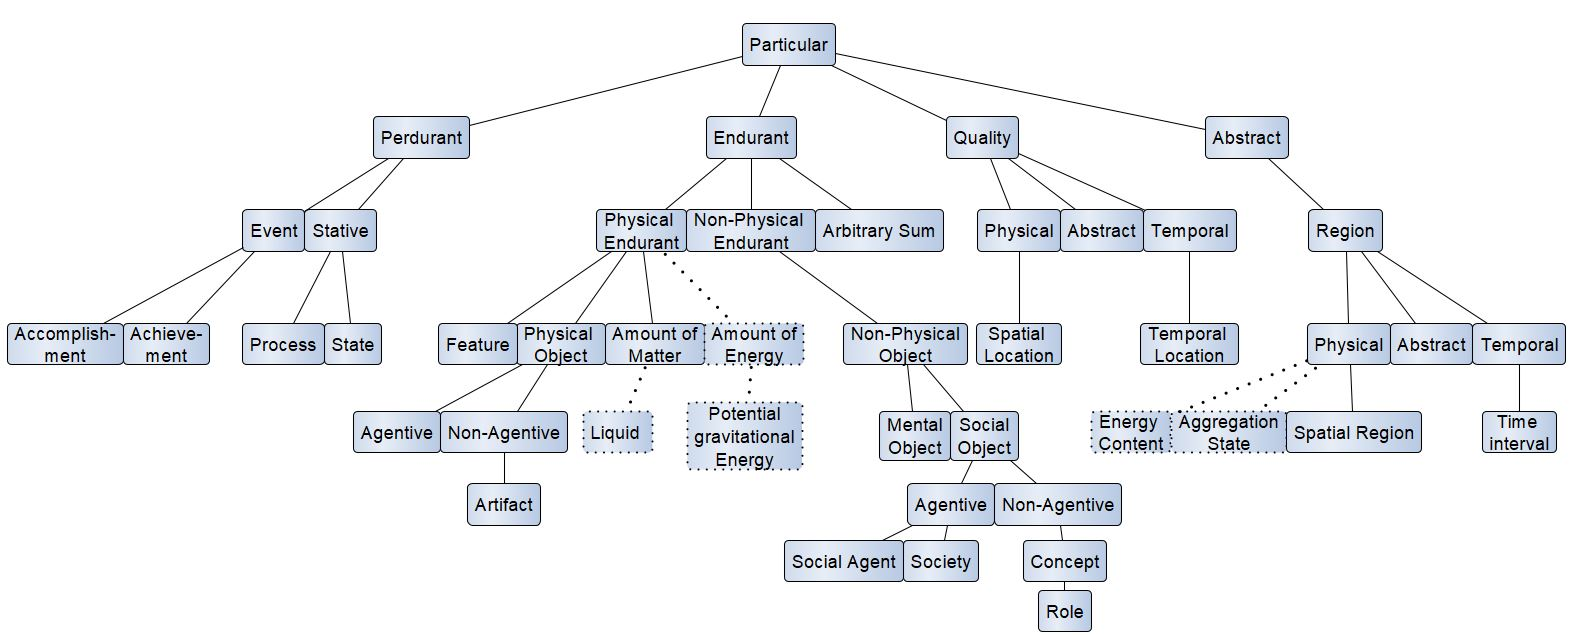
\includegraphics[width=\textwidth]{DOLCE-taxav2.JPG}
  \caption{\label{fig:DOLCE-taxa} \DOLCE taxonomy, taken from \cite{borgoDOLCEDescriptiveOntology2022}. Most divisions in subcategories are not exhaustive. The dotted classes are added to help some descriptions detailed in the paper, and are not part of \DOLCE taxonomy.}
\end{figure}

\DOLCE qualities \myComment{are similar to} were inspired by the trope theory~\cite{Campbell90} but differ from tropes in important ways. Qualities, for example the weight of a car and the color of a flower, are used for representing properties (e.g., weight) of individual objects (e.g., car) in which they inhere.
Ontologically, qualities are individuals, that is, the colors of two different flowers are different, even though they could be both the same shade of red.
Differently than tropes, qualities can change in time, for example the color quality of a flower can change its value as time passes: red in the summer and brown in the fall.
This is because values of qualities are separated from qualities themselves and are called quales. 
In this way, the assignment of values to qualities is more flexible and follows the schema object-quality-quale (or carrier-individual property-value).
In \DOLCE, qualities form the class $\generalStyle{Q}$\TODO{S: qui c'è confusione tra classe (Q) e predicato (Q(.)), ho cercato di sistemare ma il comando "DOLCEQuality" dovrebbe comparire senza parentesi. [FC: LaTeX non concede tali comodità facilmente. Ho corretto ad-hoc, ignorando il comando]} (whose predicate is written $\DOLCEQuality{\cdot}$) and the inherence relation is \quotes{quality-of} (written $\DOLCEQualityDirect{\cdot}{\cdot}$). A temporal quale relation associates a quality with some value which, as said, may be different at different times, and is written $\DOLCEQualeDirectTer{\cdot}{\cdot}{\cdot}$.% (The temporal quale relation will not be used in this paper.)

%For our purposes in this paper, 
We \myComment{add} introduce a further distinction, not present in \DOLCE, between \firstTimeKeyWord{intrinsic} and \firstTimeKeyWord{relational} (or extrinsic\footnote{
%In truth, `extrinsic' and `relational' can be used with different meanings. 
Note that the terms `relational' and `extrinsic' come from different research areas and are sometimes used with different meanings. %Due to the limited scope of our paper, we don't make such a distinction.
}) qualities
%which is not part of \DOLCE but is well discussed in the literature 
\cite{sep-intrinsic-extrinsic}. 
%to separate \firstTimeKeyWord{intrinsic} 
Standard examples of intrinsic qualities are mass, length, and shape; %and \firstTimeKeyWord{relational}, or extrinsic
of relational qualities are weight (which is a comparative property), the personal record for a marathon (which is relative to the concept of marathon), and the distance of an object from another object. %the ability of executing a certain action. 
Relational qualities are \myComment{not} qualities of an object \textit{per se} \myComment{, but} that depend on other things like another object, the context or \myComment{something in} the environment.
To clarify our intuition we illustrate some of the previous examples: the distance of the Moon from the Earth, seen as a property of the Moon, cannot be thought of nor measured without considering the Earth, so we say that it is a relational quality of the Moon (similarly, for the distance of the Earth from the Moon). In contrast, if a certain brick has a given tensile strength value, %the color of a material object, 
%as a property of the material itself, 
this fact does not depend on other entities%(not even light)
, so that tensile strength is an example of intrinsic quality; 
%Of course, this holds true only in a fixed domain of discourse, otherwise one could argue that the color too needs, say, a beam of light to be seen. 
similarly, other mechanical or chemical properties, for example ductility or the structure of the atomic lattice in crystals, can be considered intrinsic. 
Another example is the difference between weight and mass of a body: the weight also depends on the position of the body, say if the body is on Earth or on the Moon, so it is relational. 
%In addition, for someone to have a citizenship, there must be a nation the person owes its allegiance to. 
A more technical example is the voltage at a point of a component, which, since it is a potential, requires a second point used as  reference (the ground of the electrical circuit) in order to be measured. 
Informally speaking, capacities can be understood as having a relational nature, which explains our interest in the intrinsic/relational distinction across qualities. For, if we speak about the capacity of a device, say the capacity to process a certain number of items in a given time, then such capacity always refers to another entity, in this case the items.  Analogously, in \cite{qianFunctionBehaviorStructure1996}, Qian and Gero stated that there are different types of \quotes{behavioral variables}: structural, as the area of a room or the diameter of a water tap, and exogenous, as the water flow through a water tap. In the latter example, the water flow is an exogenous variable because \quotes{water is not part of the
water tap design, it is only related to the design}, so that we could argue water is an additional entity required by the water flow quality of the tap, suggesting that this form of exogeneity can be captured via our notion of relational quality.  

%behaviour can also be characterized by two kinds of behavior
%variables.
%• Structural (Direct): A behaviour is derived from the structure
%itself withouc any external effect. For example, %the
%floor of a room has an area as a behaviour %variable, which
%is directly derived frorn the room's width and %length.
%• Exogenous (Indirect): A specific kind of %behaviour is
%shown when an external object is applied to a %structure.
%For example, the waler tap or faucet has an area
%that water can pass through, but water is not %art of the
%ater tap design, it is only related to the design. The
%water flow is an indirect behaviour variable %controlled
%by the diameter of the water tap. --Qian, Gero 1996

In the previous examples, it seems that relational qualities are those qualities that depend, in some way, on an entity different (we say \firstTimeKeyWord{external}, see \refdf{def:external}) from their bearer. Unfortunately, the exact meaning of this dependence relation changes between the different examples. In particular, in the case of capacities the dependence is `potential', for a device can have the capacity to process a product, even when the product is not actually present. In contrast, in the case of relative distance the dependence is `actual', for a physical object is at any time at a certain distance from another.\footnote{Note that relative distance makes sense only at times in which both objects exist.}
It follows that the characterisation of relational qualities is a complex matter that goes beyond the scope of this paper.\footnote{The interested reader can find a proposal on relational and intrinsic qualities in \cite{fonsecaRelationsOntologyDrivenConceptual2019}.} Therefore, we introduce intrinsic and relational qualities as primitive predicates that partition the class \DOLCE-qualities: 
\bflist
  \item[\myax{relationalQtPartialDef}] $ \RelationalQuality{x} \myfi \DOLCEQuality{x} $ 
  \item[\mydf{intrinsicQtPartialDef}] $ \IntrinsicQuality{x} \myiff  ( \DOLCEQuality{x} \land \neg  \RelationalQuality{x})$
  %\item[] \mytext{$x$ is an intrinsic quality if and only if it is a quality and it is not relational}
\eflist



Turning now to perdurants ($\DOLCEPerdurant{\cdot}$)\myComment{, which we will also refer to as occurrents in this paper\TODO{S: perché creiamo questa potenziale confusione terminologica? possiamo evitarla?[FC: sì, l'unica cosa è che ogni tanto il verbo 'to occur' no ha alternative. Però i sostantivi 'occurrent(s)' si potrebbero sostituire coi sostantivi 'perdurant(s)']}}, in \DOLCE they are entities that are only partially present at any time they are present.\footnote{Ordinary physical objects such as cars, trees, rocks, etc. are considered fully present at every time in which they exist.} For example, a chemical process, the lifting of a load, and a sitting action are only partially present at each instant at which they happen. Indeed, the initial part of a chemical process is not present when the process reached the midway point, and vice versa.  %only when considered with their full time extension. 
\DOLCE uses three mereological properties to distinguish perdurants: cumulativity, homeomericity, and atomicity.
Cumulativity holds if the sum of two instances of a type has the same type, that is, if the type is closed under mereological sum. Consider, for example, \quotes{walking}: if we consider two walking activities, then the activity that comprises both is still an activity of type \quotes{walking}.
Cumulative perdurants\footnote{More precisely, instances of a cumulative type perdurant.} are called \firstTimeKeyWord{stative} ($\DOLCEStative{\cdot}$), while the ones that are never cumulative are called \firstTimeKeyWord{eventive}.
Homeomericity holds for a perdurant type if any parts of its instances are instances themselves.
This is the case of, e.g, \quotes{sitting}, since portions of a sitting action are still sitting actions.
Stative homeomeric perdurants are called \firstTimeKeyWord{states} ($\DOLCEState{\cdot}$), while the ones that are stative but have parts of different type are called \firstTimeKeyWord{processes}($\DOLCEProcess{\cdot}$). Walking itself is an example of process in \DOLCE: walking requires at least to complete a certain leg movement, below such granularity is not a walking movement.
Another example is the buzzing of a clapper (or buzzer): the clapper alternates between two states when clapping (opened/closed circuit), and neither state is per se of buzzing type. In \DOLCE the temporal relationship between a perdurant and the object participating in it is called \firstTimeKeyWord{participation}, written $\DOLCEPC{\cdot}{\cdot}{\cdot}$: in the previous example a participant of the buzzing is the clapper.

%%%%% old paragraph
% Finally, roles are not mentioned in \DOLCE, but they are used in the related literature, at the meta level, as labels for classes \cite{guarinoOverviewOntoClean2009, guarinoFormalOntologyProperties2000}.
% A class is a role whenever its instances are not necessarily so and, moreover, they depend on some external context (external meaning that is not a part of a substrate). 
% For example, a certain person could be a student, but not necessarily so, in fact, if it is a student, we expect for it to cease to be a student after some time. 
% Additionally, a student is such only in the context of a certain school.
% Oppositely, any person is necessarily so, and it is independent of other external entities.
% We will not introduce a category for roles, instead, in the following, we will sometimes label a class as a role. 
% Whenever we do that, we mean it as a meta-logical label, as explained before. 
%%%%%% new paragraph
Coming to roles, they were not covered in \DOLCE originally. They have been introduced later as an extension \cite{masoloSocialRolesTheir2004}, and are now part of the expanded taxonomy \cite{borgoDOLCEDescriptiveOntology2022}.
Roles are antirigid and dependent (aka founded) classes \cite{guarinoOverviewOntoClean2009, guarinoFormalOntologyProperties2000,masoloSocialRolesTheir2004}. 
A class is antirigid whenever its instances are not necessarily so, and is dependent if all of its instances (existentially) depend on some external entity, often called context.
For example, a certain person can be a student, but no person is necessarily a student. Actually, we expect that a student ceases to be such after some time. 
In contrast, any person is necessarily a person, and is so independently of other external entities.
%Additionally, a student is such only in the context of a certain school.
An ontological class (existentially) depends on, or is founded on, another if, whenever an instance of the first class is present, a corresponding instance of the second is present too.
For example, for every citizen there is a country, so that someone's citizenship depends on the country. Actually, in this paper, we will be more precise and distinguish between different kinds of dependence and founding, but the basic idea is still captured by the citizen-country example. 
Additionally, some authors divide roles depending on the type of their context, 
for example \cite{loebeAbstractVsSocial2007} distinguishes relational, processual, and social roles. The classification depends on whether the context is a relation, a process, or a social object. 
In \DOLCE, roles ($\DOLCERole{\cdot}$) are reified and considered as concepts ($\DOLCEConcept{\cdot}$), which themselves are a class subsumed by the class of non-agentive social objects ($\DOLCENASO{\cdot}$):
\bflist
  \item[\myax{roleSussum}] $ \DOLCERole{x} \myfi \DOLCEConcept{x}$
  \item[] \mytext{a role is a concept}
  \item[\myax{roleSussum2}] $\DOLCEConcept{x} \myfi \DOLCENASO{x}$
  \item[] \mytext{a concept is a non-agentive social object}%\TODOinline{[SB: ho spezzato][FC:ok]}
\eflist
In this paper, the fact that roles are founded is particularly important, thus, we give the following formalisation, where $\DOLCECLby{\cdot}{\cdot}{\cdot}$\marginpar{\color{red}{ho sostituito CL con CF}} (`classified-by', also called `play-as', if the first argument is a role) is the classification relation between a concept and its instances at a certain time, cf. \cite{masoloSocialRolesTheir2004}. In the formalisation we use some other relations taken from \DOLCE, namely: constitution, $\DOLCEK{\cdot}{\cdot}{\cdot}$,
 which is the  relation holding between some amount of matter and an object when the latter is made of the first (e.g., a statue and the amount of clay it is made of);  $\DOLCEOverTemp{\cdot}{\cdot}{\cdot}$, which is the standard overlap relation (over time) (e.g., two semi-detached houses overlap because of the wall they share); and $\DOLCEPRE{\cdot}{\cdot}$, which is the relation "being present (exist) at time". %, and $\playAs{\cdot}{\cdot}{\cdot}$ is its restriction to roles:
\bflist
\item[\mydf{external}] $ \external{x}{y} \myiff \neg (\DOLCEQualityDirect{x}{y} \lor \exists t(\DOLCEK{x}{y}{t}) \lor \exists t(\DOLCEOverTemp{x}{y}{t}))$
\item[] \mytext{$x$ is external to $y$ if and only if $x$ is neither a quality of $y$, nor one of $y$'s constituents
%\footnote{Constituent, or substratum, as in \quotes{this fork is constituted by stainless steel.}}
(at any time), nor $x$ and $y$ have parts in common\footnote{Substrata, parts, and qualities may not cover all possibilities especially if a different top-level ontology were used.} (at any time)}  
%\TODO{rendere la relazione simmetrica?}
%Here, the dependence relationship is specific and constant, that is,
%$x$ depends on $y$ if and only if whenever $x$ exists, so does $y$: 
\item[\mydf{specificallyDependsOn}] $ \specificallyDependsOn{x}{y} \myiff (\exists t(\DOLCEPRE{x}{t}) \land \forall t(\DOLCEPRE{x}{t} \myfi \DOLCEPRE{y}{t}))$ 
\item[] \mytext{$x$ existentially depends on $y$ if and only if $x$ exists at some time and at any time when $x$ exists so does $y$}\footnote{The existential quantifier is a technicality: without it an entity that is never present would depend on all entities. Similarly, existential quantifiers are introduced in axioms having a similar structure to this one.}
\item[\mydf{foundingBasic}] $ \founded{x}{y} \myiff (\specificallyDependsOn{x}{y} \land \external{x}{y})$
\item[] \mytext{$x$ is founded on $y$ if and only if $x$ existentially depends on $y$ and $y$ is external to $x$} 
\eflist
Further, we specialize the founding relationship to concepts and their instances as follows:
\bflist
\item[\mydf{founding}] $ \foundedROLE{x}{y} \myiff (\DOLCEConcept{x} \land \exists z,t (\DOLCECLby{z}{x}{t}) \land \forall z,t (\DOLCECLby{z}{x}{t} \myfi \exists w (\founded{z}{w} \land \DOLCECLby{w}{y}{t})))$
%\textcolor{blue}{(e' necessario assumere che il concetto classifichi qualcosa (quantificatore esistenziale)?(FC: argomentabile, vedi nota 18)( cmq farei un esempio con $founded_{cn}$)(FC: inserito sotto esempio husband-marriage, è OK?)(SB: meglio tenerlo per evitare casi di foundedness irrilevanti)}
\item[] \mytext{the concept $x$ is instantiation-founded on the concept $y$ if and only if, given any $z$ that plays $x$, then $z$ is founded on some instance of $y$} 
%that is, instantiation-founding is the founding relation `lifted' to concepts. Note that the without the existential quantification any empty concept would be founded on every other concept.

\item[\myax{roleFounding}] $ \DOLCERole{x} \myfi \exists y~ \foundedROLE{x}{y} $ 
\item[] \mytext{if $x$ is a role, then there is a $y$ on which it is instantiation-founded} 
%cfr. \refax{ax:relationalQtPartialDef}.
\eflist 
For example, the role of `husband' is instantiation-founded on the concept of `marriage', since every time a person is a husband there is an individual marriage between that person and another person.\marginpar{\color{red}{Questo esempio va ampliato per esemplificare la formula d5 in modo sistematico.}}

We also need to capture a different kind of founding relation, that we call \firstTimeKeyWord{definition-founding} ($\foundedDef{\cdot}{\cdot}$). We do not formalize this relation as it requires discussing how to formally define roles, a topic beyond our concerns in this paper. We will use it with the following informal interpretation: \mytext{$x$ is definition-founded on some entity $y$ if and only if $y$ is used to define $x$}.
%\TODOinline{[assumo che applichiamo la relazione solo a concetti, confermi?][FC: no, perché la ragione di introdurre questa relazione è la definizione \refdf{def:capability}, per provare a collegare le capability alle funzioni.][SB: ok, ho tolto le restrizioni a "concept" nel testo][FC:roger]} 
For example, if a doctor is defined as a person who treats sick people, then the doctor-role is definition-founded on the sick-person concept. %\TODO{S: userei "sick person" per evitare che la relazione founded sembri simmetrica: a doctor is defined as a person who treats people which are in a sick state [FC:Ok]}  %and we will enforce only the following axiom:
%\bflist
%\item[\myax{foundingDefRange}] $ \foundedDef{x}{y} \myfi \DOLCEConcept{y}$\footnote{A more in-depth discussion of definition founding, usually called definition dependence, can be found in \cite{masoloSocialRolesTheir2004}.} 
% \eflist 
Note that instantiation-founding and definition-founding need not  coincide. A person is a doctor even though, at a certain time, she is not treating any sick person: the doctor-role is not instantiation-founded on someone being in a sick state\TODO{S: on someone being in a sick state}.

Finally, since roles, as well as concepts, can be seen as reified classes, there exists a specialisation relation between roles, which we write as $\DOLCEConceptSubsum{\cdot}{\cdot}$:
\bflist
\item[\mydf{conceptSussum}] $ \DOLCEConceptSubsum{x}{y} \myiff (\DOLCEConcept{x} \land \DOLCEConcept{y} \land \exists z,t (\DOLCECLby{z}{x}{t}) \land \forall z,t (\DOLCECLby{z}{x}{t} \myfi \DOLCECLby{z}{y}{t}) )$%\footnote{Note that, technically, \refdf{def:conceptSussum} entails that any empty concept specialises any other concept. This is not important, since we do not care about empty concepts.}
\item \mytext{A concept $x$ specializes a concept $y$ if and only if all instances of $x$ are also instances of $y$} 
\eflist
For example, the role of the Italian Prime Minister specializes the role of Prime Minister.
{This notion of specialisation is admittedly weak. One would like to add a modal characterisation: definition \refdf{def:conceptSussum} should hold in all possible worlds. This problem applies to other definitions we introduce in this paper %and in some special cases we will discuss this issue.
and is not ontological but related to the limitations of first-order logic. Without discussing logical technicalities, in this paper we will make use of these characterisations assuming that, in suitable systems, e.g. first-order modal logic, a suitable formula is substituted.}

%%%%%%%%%%%%%%%%%%%%%%%%%%%%%%%%%%%%%%%%%
\section{Modelling behaviours and functions in \DOLCE \label{sec:capabilitiesEtc}}
%%%%%%%%%%%%%%%%%%%%%%%%%%%%%%%%%%%%%%%%%
%%%% Inizio formalizzazione
%% formalizzazione parte 1: entita' di base e loro mereologia
%Our investigation involves engineering systems and devices. 
In this section we propose a framework to characterize how behaviour and function of engineering artifacts can be understood to make sense of the distinctions used by engineers in different areas, from engineering design to manufacturing and maintenance, from process planning and product planning to early system design planning. Within the following section, we will expand this view to capability and capacity.
%In this work we use \DOLCE as our top-level ontology.

In the literature, many terms are used to refer to engineering systems and devices such as part, component, tool, machine, (technical) artifact, functional object etc. 
We use \firstTimeKeyWord{technical artifact}\footnote{See \cite{borgoTechnicalArtifactsIntegrated2017} for a more in-depth discussion of technical artifacts.} to mean any physical object (see \refax{ax:subsumptionTArt}) that comes into being through an intentional technical process, such as, e.g., cars, planes, tooling machines and, more generally, devices designed to perform tasks. %Sometimes we will use \quotes{device}, \quotes{artifact}, and,  especially when we want to highlight the mereological structure of an artifact, \quotes{system} as synonyms.
Also, we will use the terms \quotes{device} and \quotes{technical artifact} as synonyms. 
Additionally, we will use the term \firstTimeKeyWord{system} in order to highlight the mereological structure of a complex artifact. 
%In reality, %\myComment{truth}\textcolor{blue}{( `in truth' e' molto italiano ;)},
The notion of system is complex, cannot be reduced to  that of technical artifact, and its precise characterisation is an open problem (see e.g. \cite{mizoguchiRoleSystemicView2021}). In the paper, we take this notion as given introducing a primitive class, $\System{\cdot}$. In particular, technical artifacts belong to this class. 
%especially if they are the object of teleological analysis. \textcolor{blue}{( serve parlare di System? artefatti mereologicamente complessi per i quali si specificano le funzionalita'? Lo stesso non puo' gia' valere per TechArt?)}
%[SB: hai ragione. una bozza di caratterizzazione c'è nell'articolo di Riichiro e me in JOWO 2021. è poco ma è un inizio. purtroppo non riesco a metterci un po' di tempo per sviluppare di più quell'idea (che è sostanzialmente di Riichiro). Cmq la noz. di funzione sistemica presuppone che ci sia una nozione di sistema. quella di artefatto è troppo debole. direi di fare riferimento a quell'articolo a JOWO, dicendo che per ora assumiamo la nozione ma che resta aperto il problema di caratterizzarla in modo adeguato.]
%%Definition 3 (System and its Components). A system is an entity which consists of two or more identified components and their relationships. The components can be atomic or complex. An atomic component is not decomposed further. A complex component is itself a (sub-)system. Every system is decomposed into atomic components in a finite number of steps -- estratto da Borgo&Mizoguchi 2016, in 2021 è cambiato:
\begin{comment}
A generic system as a Structure (See 2.3) is an entity such that:
(i) is a whole (physical) entity with a boundary separating the world in: the system’s inside and the
system’s outside (the latter can be possibly empty if the system is the universe itself).
(ii) has one or more components (the simplest case is, e.g., a pebble as a paper weight)
(iii)if it has more than one component, each of its components must interact with at least another
component. More precisely, a multi-component system cannot be divided in two non-interacting
subsystems.
(iv) if it has more than one component, it can be decomposed into multiple subsystems.
(v) if it has more than one component, the systemic goal of a subsystem is specified by its smallest
super subsystem. Intuitively, it is a (possibly non-intentional) goal necessary for sense-making
the behaviour of a subsystem. As described above, it is automatically specified when the behaviour
of the system is selected because all the components are supposed to realize the behaviour.
(vi) has input object(s) which is processed and then output.3 By being processed, we mean: a
quality/state of the input object is changed while it goes through the subsystem. The completion
of the process with the output release4 achieves the systemic goal. The detail of the process is
defined in the Device ontology discussed in section 3.B).
(vii) its connected components exchange information or objects as input/output.
(viii) its subsystems are also systems.
\end{comment}
The mereology mentioned above is built as usual from the temporalized parthood relation of \DOLCE,  $\DOLCEPart{\cdot}{\cdot}{\cdot}$. \DOLCE defines also a non-temporalized parthood relation, $\DOLCEPartBin{\cdot}{\cdot}$, given in \refdf{def:partConstant}. Axiom \refax{ax:part-present} and the class $\DOLCEPhysObj{\cdot}$, the category of physical objects, are also taken from \DOLCE.
\bflist
\item[\myax{subsumptionTArt}] $ \TechArt{x} \myfi \DOLCEPhysObj{x}$
\item \mytext{a tecnical artifact is a physical object}
%\footnote{One could argue that technical articfact can also be perdurants [...].} 
\item[\mydf{partConstant}] $ \DOLCEPartBin{x}{y}  \myiff \exists t (\DOLCEPRE{y}{t}) \land \forall t (\DOLCEPRE{y}{t} \myfi \DOLCEPart{x}{y}{t})$
\item \mytext{$x$ is constantly part of $y$ if and only if whenever $x$ exists, it is part of $y$}
%this is a standard way of removing the temporal argument from parthood
%Finally, we will use the fact that only actually present objects can be part of other objects:
\item[\myax{part-present}] $ \DOLCEPart{x}{y}{t} \myfi (\DOLCEPRE{x}{t} \land \DOLCEPRE{y}{t})$
\item \mytext{if $x$ is part of $y$ at time $t$, then $x$ and $y$ are both present at time $t$}
\eflist
%\textcolor{blue}{(per quanto possa dirne io, in genere le formule vengono sempre richiamate nel testo, cosa che nell'articolo non si fa sempre)}

%% formalizzazione parte 2: introduzione di capabilities e capacities
%%--> posticipato. Controllare tutto!!!



%%%%%% formalizzazione parte 2: comportamenti
\subsection{Behaviours}
%In the previous examples, the relational qualities refer to a specific type of external entity, namely perdurants (like jumping, pumping, the functioning of an electrical circuit) in which the bearing object participates. 
%Engineers are often focused on realizing specific interactions between an artifact and elements of its environment. 
Engineers create an artifact to realize a certain interaction between the artifact itself and elements of the environment. The behaviour of the artifact is the way in which it participates in the interaction (e.g. \quotes{[the car] rattled when it hit the curve} ~\cite{chandrasekaranFunctionDeviceRepresentation2000}). 
In \DOLCE one models the happening of the interaction as a perdurant. How to ontologically understand behaviour is more tricky. 
%Informally, it is the participant's way of being in the perdurant.  in the perdurant \cite{borgoFormalOntologicalPerspective2009} (the participant in the previous example would be the car).
In the literature, the term behaviour is used with different meanings, e.g., as simplified part or description of processes like in these excerpts: \quotes{The causal rules that describe the values of the variables under various conditions} \cite{chandrasekaranFunctionDeviceRepresentation2000}, \quotes{the behaviour represents objective conceptualisation of its input-output relation as a black-box} \cite{kitamuraOntologicalModelDevice2006}, \quotes{situation-independent conceptualisation of the change between input and output of the device} \cite{mizoguchiFunctionalOntologyArtifacts2009}. 
In \YAMATO \cite{Mizoguchi2017YAMATOYA} behaviours are modelled as processes with an \quotes{agent or an agent-like object as a doer}. 
Instead, in \cite{borgoFormalOntologicalPerspective2009} Borgo et al.  model them as relational qualities which characterize the specific way of participation of an object in individual events. 
%The latter choice entails the use of a ternary relation, since it treats behaviours analogously to adverbs, that is, predicates about the participation relation of an object in a process itself. 
%\TODO{riscrivere questo paragrafo, also per SB adesso sono qualità relazionali}
%Since we want to minimize the complexity of our formal language, we discard this modelling choice.

% % % % % % % %% % % % %% % % % PARAGRAFI RIMOSSI PERCHE' NON ANDAVANO DA NESSUNA PARTE
% % Instead, we develop the following construction in order to define what a behaviour is.
% % First, we say that \firstTimeKeyWord{system} is the role that a technical artifact plays whenever it is studied as the object of teleological analysis by an engineer or a scientist.
% % A system has, as it is, a countless number of qualities that we can think of.
% % For example, at each and every point of the artifact we could take the temperature, the density, the color, etc. 
% % These are already an infinite number but, of course, an engineer or scientist that studies the artifact only selects some of them, that we call \firstTimeKeyWord{state variables}\footnote{State variables are roles of regular qualities.}\footnote{Note that, often, but not always, the state variables of a system coincide with some variables of the underlying artifact. For example, the temperature at a given point is a quality of the artifact and (thus) of the system, while the input current of, say, an amplifier, is not %\TODO{is it not?}}.

% % Each observer could select a different set of variables, in that case there would exist different systems and those variables would belong to a system but not another, thus those systems would necessarily be different entities.
% % Such systems would also be co-located, since they would be made from the very same underlying technical artifact. 
% % Therefore, we can manage such cases by making use of the technique of \firstTimeKeyWord{entity stacking}, exploiting the multiplicative approach of \DOLCE \cite{vieuArtefactsRolesModelling2008}.
% % Though, for simplicity, in the following we will assume %\TODO{will we?} that there is a fixed point of view, so that to a single artifact corresponds a single system.

% % Finally, we assume that a system can have smaller systems as parts, where the part-whole relation is lifted from the corresponding relation between technical artifacts.
% % We also assume that, whenever a subsystem has a state variable, that quality is also a state variable of the entire system. 

% % Note that not all subsets of parts are subsystems: they could be, but, in general, it depends on the choices carried out by the observer. 
% % In fact, they select some subsets of components as subsystems, depending on the their goals, in a way that we will explain in the following %\TODO{assicurarsi che sia stato fatto}. 
% % \bflist
% %   \item[\myax{systemSubsum}] $ \System{x} \myfi (\DOLCEPhysObj{x} \land \exists y (\TechArt{y} \land \DOLCEConstitutes{y}{x}) $
% %   \item[\myax{stateVarSubsum}] $ \StateVariable{x} \myfi \DOLCEQuality{x} $
% %   \item[\myax{subsystemPartDef}] $ \partS{x}{y} \myiff (\partTA{z}{w} \land \DOLCEConstitutes{z}{x} \land \DOLCEConstitutes{w}{y} \land \System{x} \land \System{y}) $
% %   \item[\myax{stateVarInheritance}] $ (\partS{x}{y} \land \inheres{z}{x} \land \StateVariable{z}) \myfi  \inheres{z}{y} $ %% TODO %\TODOinline{\text{forse e' necessario un predicato binario per le variabili di stato?}}
  
% % \eflist

% % State variables are the qualities that engineers and scientists take into account when simulating a system. 
% % For example, one could simulate an electronic system and measure the voltage in a point, say the output voltage of a signal generator. 
% % Then one can check if the voltage stays constant in time, if it increases or decreases, if it oscillates, or if it does something more complex\footnote{Note that we use examples from the engineering domain, but one could, without any change, think about biology, for example considering the fact of someone's fingers being black, following severe exposure to cold %\TODO{check se ha senso}.}.
% % In any case, such changing of the values of one or more state variables are stative perdurants\footnote{See Paragraph \ref{par:DOLCE}. For example, two increasing are still an increasing, so they are statives; a portion of increasing is still an increasing, so they are states. Oscillating is a process, etc.}, because a composition of changings of some variables is still a changing of some variables.
% % Of course, in the literature such changings are called \quotes{states}, but we cannot do that, since in \DOLCE they are really stative perdurants.
% % Therefore, we shall use the term \textit{\stateVarCond{fullPlural}}.
% % %we need to use \quotes{stative perdurant} insteaad, since that is the correct DOLCE category. 

% % Notice that each \stateVarCond{fullSingular} only carries a part of the system information.
% % One could say that it is a view of the whole \stateVarCond{shortSingular} of the system imposed by the engineer or scientist that observes the system.
% % So that the whole condition of the system completely specifies it, while any other \stateVarCond{fullPlural} is less informative. Thus, if we conceptualize the fact of being more or less informative with a part-whole relation between \stateVarCond{shortPlural}, we can define the whole \stateVarCond{fullSingular} as the one that is maximum with respect to the mereological order.
% % Following common terminology, we call the maximum of \stateVarCond{fullSingular} \firstTimeKeyWord{(complete) behaviour of the system}.
% % \bflist
% %   \item[\mydf{behDef}] $ \behaviourOf{x}{y} \myiff  (\DOLCEPC{y}{x}{}\land \\ \forall z (\StateVariableCondition{z} \land \DOLCEPC{y}{z}{} \myfi \DOLCEPart{z}{x}) \\ \text{%\TODO{vedere se mettere fusione invece}}$
% % \eflist
% % %Definition \ref{def:behDef} entails that the behaviour of a system is unique.

% % Now, not all expressible \stateVarCond{fullPlural} are possible: some could be logically inconsistent (e.g., the temperature is plus 20 and minus 2 degrees Celsius), some could be outside the realm of physics (e.g., a temperature in negative Kelvin degrees). The remaining are the possible \stateVarCond{shortPlural}. 

% % Engineers and scientists, that reason about the workings of a system, typically select a possible \stateVarCond{fullSingular}, that is actually happening or only thought of, and wonder what
% % has caused it to happen\footnote{%\TODO{elaborare sulla causazione: la fisica puo' fornire delle leggi matematiche tra le variabili e i lori cambiamenti. Queste pero' non necessariamente recano informazioni causali, e.g., le leggi aritmetiche o certe leggi differenziali non hanno informazione causale. Si puo' argomentare che alcuni cambiamenti accadono prima e altri dopo, ma questo e' vero solo per misure prese in punti diversi  (B1 behaviours), ma, sopratutto, potrebbe accadere così velocemente che l'osservatore non se ne accorge.}}.
% % This is an essential step, since it introduces a `causal order' between a system \stateVarCond{shortPlural}, that could otherwise not be present.
% % More precisely, we say that an observer selects some particular \stateVarCond{fullSingular} as \firstTimeKeyWord{goal}, goals being roles for \stateVarCond{shortPlural}, in order to explain what causes the goal to happen.

% % Typically, if an observer selects a goal and just a single other \stateVarCond{fullSingular}, the other \stateVarCond{shortSingular} is not enough to build a causal explanation for the goal: other information are needed. 
% % The complete behaviour of the system is certainly sufficient to explain the causation, but it is often impossible to known for the observer. 
% % % % % % % %% % % % %% % % % PARAGRAFI RIMOSSI PERCHE' NON ANDAVANO DA NESSUNA PARTE - FINE 

%%%%% definizione generale di comportamento
%It is difficult to give a definition of behaviour, due to the many uses found in the literature.
%We will still give a definition, since it is necessary to carry on our analysis, but, more importantly, 
Here we discuss a few key ontological properties to distinguish possible definitions of behaviour.
There are, in fact, at least four %\TODO{[four?][FC:yes]} 
axes along which different meanings of behaviour can vary in the literature.
First, there is what we call the occurrence-property dichotomy:
\begin{itemize}
  \item behaviour can be something that happens in time \myComment{(occurs)} and in which the behaving entity participates, 
  in this case it is typically referred to as a transition between states or just as (staying in) a state. 
  Examples are provided by Goel \cite{goelStructureBehaviorFunction2009}, Chandrasekaran \cite{chandrasekaranFunctionDeviceRepresentation2000}, Umeda \cite{umedaFunctionBehaviourStructure1990}, and \YAMATO authors' \cite{mizoguchiFunctionalOntologyArtifacts2009}.
  \item behaviour can \myComment{also} be a property, that is, something inhering into the behaving entity. 
  \myComment{In this case some authors speak of} Examples are provided by Borgo et al. in terms of qualities \cite{borgoFormalOntologicalPerspective2009}, Vermaas or Gero and colleagues in terms of attributes or dispositions \cite{vermaasConceptualFrameworkJohn2007}, \cite{geroCategorisingTechnologicalKnowledge2002}.
\end{itemize} 

Then, there is the token-type distinction: behaviour can be a class or a concept, as for  Mizoguchi in \cite{mizoguchiFunctionalOntologyArtifacts2009}. Alternatively, it can be an instance of something, or an entity relative to a specific event, as for Chandrasekaran and Josephson in \cite{chandrasekaranFunctionDeviceRepresentation2000}, and for Borgo et al. in \cite{borgoFormalOntologicalPerspective2009}, respectively. 

Additionally, there is the external-internal axis, that is, the behaviour of an artifact may refer only to characteristics of the artifact itself, or it may need to refer to \myComment{some} external entities.
For example, `the electric switch can alternate between open and closed states' is an internal behavioural description, as it refers only to transitions between states of the artifact.
In contrast, `the current passing through an open switch is zero, if the applied voltage stays within operating conditions' is an external description, since, the current and the voltage are not intrinsic elements of the artifact. %\TODO{intrinsic qualities??? SB: non direi visto che qui behaviour non è necessariamente una qualità, certo può esserci un legame}.
Some authors explicitly use behaviour with the internal meaning, e.g. Zhao et al. in \cite{zhaoStateBehaviorFunction2019}, others with the external one, as Kitamura et al. in \cite{kitamuraOntologybasedSystematizationFunctional2004}.%\textcolor{blue}{(usate sia \& sia et, meglio adottare la seconda opzione secondo me)(FC: sostituito Tizio \& al. con Tizio et al. e Tizio \& Caio con Tizio and Caio)}.

Finally, there is the modal axis, since \myComment{for \textcolor{blue}{(since? considering that?)}} behaviours can be \myComment{\textcolor{blue}{(either)}} either expected (i.e. as envisioned by engineers) or actual (i.e. what actually happens), as implied by Gero in \cite{geroSituatedFunctionBehaviour2004} with respect to design activity (though one could use the same duality when talking of, e.g., malfunctioning).
This axis includes, arguably, talks of causal laws or relations, since those could be conceptualized as changes of a system under some kind of %epistemic 
modality, that is, changes that necessarily happen when some condition is met.
We do not argue in favor of conceptualizing causal laws in this way, but, in any case, one must also take this use of behaviour into account, since it is encountered often. %often.
%Other differences exist in the literature, such as device-centric vs. environment-centric \cite{chandrasekaranFunctionDeviceRepresentation2000}, but we do not discuss them. \marginpar{questo rientra in external-internal}

%By virtue of how our approach is structured, to define behaviour as a property would make it very similar to a capability, or to the realisation of one.
%\TODO{[FC: completamente ristrutturato questo e i prossimi paragrafi. Tengo "behaviour $\subset$ Perdurant" con una caratterizzazione parziale perché è quella più vicina all'uso in ingegneria]}


%\TODOinline{[Ho tolto la discussione su (ex1), può generare confusione e non serve per i nostri scopi]}
%Following common practice in the literature, in this paper we define behaviours as perdurants. 
% More precisely, one could be tempted to subsume the class of behaviours in the category of \DOLCE processes, since behaviours are usually called \quotes{processes}:
% \bflist
% \item[\myex{behaviorSubsum}] $ \BehaviourConcrete{x} \myfi \DOLCEProcess{x} $
% \eflist
%However, this should be done only under specific assumptions, e.g., if one were to capture the use of `behaviour' as discrete transitions between states. In fact, in that case, one may assume that the cumulativity property holds, since the composition of two transitions between states is still a transition between states, and homeomericity does not, since there will always be a temporal part of a (discrete) transition between states that is not a transition between states. Therefore, the choice of \refex{ex:behaviorSubsum} is compatible with, e.g., representing transitions as discrete `jumps' between states, and with Kitamura et al.'s B1 behaviors%\TODO{[non sono stati introdotti i behaviour B1, dobbiamo dire qualcosa o eliminare la nota...]*[FC:sono stati introdotti sopra]*[SB: ma era solo un cenno, non c'è info sufficiente per il lettore per capire, almeno aggiungi un paio di esempi positivi e un esempio negativo...][FC:hai ragione, aggiunti esempi]}
%\footnote{For, in the case of B1 behaviours, we argue that there is a minimum time duration for the behavior: the time necessary for the operand to move between input to the output ports}. For those same reasons, choosing \refex{ex:behaviorSubsum} excludes transitions that are not happening along a continuum, thus it cannot be assumed \textit{a priori}.  
%We will always mention if we speak about a token or a type %\TODO{<---check if true and if really needed FC: rimosso}.
%We understand %\TODO{riscrivere frase} that any given device type can participate only in some behaviour types and not other, for example, a hammer will never participate in a process 
%Furthermore, we will not specify a position on the external-internal axis or on the modal one, because it would be outside the scope of this paper and to allow for the biggest number of possible extensions of our theory. %\TODO{chechk}

%The previous discussion shows that caution is required when choosing what ontological properties of behaviours hold. 

\medskip
\myComment{Following common practice in the literature, 
in this paper} 
%We take behaviours to form a subclass of \DOLCE perdurants. 
In this paper, we take behaviours in engineering to be a role-based reading of a subclass of \DOLCE perdurants. 
This class is partially characterized by the fact that one can identify two `processual'\footnote{Note that the term \quotes{processual role} refers to general perdurants, it is not limited to \DOLCE processes. The terminology is taken from Loebe which introduces it relatively to the GFO approach \cite{loebeAbstractVsSocial2007}.} roles in the sense of \cite{loebeAbstractVsSocial2007}: an active one, called \firstTimeKeyWord{doer}, and a passive one, called \firstTimeKeyWord{operand} or \firstTimeKeyWord{flow} \cite{pahl_engineering_2007}.\footnote{The view of behavior as a relational quality between an entity and its environment \cite{borgoFormalOntologicalPerspective2009} is ontological and applies broadly, not only to the engineering domain. Nonetheless, the role-based notion of behavior that we adopt here, is more natural in the context of functional modeling.} 
For instance, a cutting action entails that there is something that is the subject of the action, say a saw (or the system formed by a person or machine using the saw), and the object of the action, say a beam of wood.
The same holds for pumping, joining, and other behaviours that can be described by transitive verbs. 
In fact, all devices' behaviours that can be described as operations on flows are of this kind. 
Such behaviours, whose class we characterize with predicate $\BehaviourConcrete{\cdot}$, are external behaviours, since the flow is an entity external to the behaving artifact (the doer).
We conceptualize the two processual roles through two specialisations of the participation relation: $\participateAsDoer{\cdot}{\cdot}{\cdot}$, to indicate participation in a process with the role of an agent or agent-like doer, and $\participateAsFlow{\cdot}{\cdot}{\cdot}$, for the role of flow: 
\bflist
  \item[\myax{participateAsDoerRage}]  $ \participateAsDoer{x}{y}{t} \myfi (\TechArt{x} \lor \DOLCEAgent{x} ) \land \BehaviourConcrete{y} \land \DOLCEPC{x}{y}{t}$\TODO{S: non dovremmo escludere persone/operatori, meglio dire "$\TechArt{x} \lor \DOLCEAgent{x}$" [FC:ok]}
\item \mytext{if $x$ is a doer in $y$ at time $t$ then $x$ is a technical artifact or an agent, $y$ is a behaviour, and $x$ participates in $y$ (in the \DOLCE sense) during that time}
  \item[\myax{participateAsFlowRage}]  $ \participateAsFlow{x}{y}{t} \myfi \myComment{(\DOLCEPhysObj{x} \lor \DOLCEQuality{x} \lor \texttt{AOM}(x)) \land} \BehaviourConcrete{y} \land \DOLCEPC{x}{y}{t}$
\item \mytext{if $x$ is a flow in $y$ at time $t$ then $y$ is a behaviour, and $x$ participates in $y$ during that time}%\footnote{We do not commit to a classification of flows into some categories, since we want our theory to be flexible enough to consider physical objects, substances, and qualities (cfr \cite{borgoFormalizationFunctionsOperations2011}), but also other entities such as events or information.}\todo{S: qui x non può essere un evento a causa di PC(x,y,t)}
  \item[\myax{processualRoles}] $ \BehaviourConcrete{x} \myfi \exists y,z,t(\participateAsDoer{y}{x}{t} \land \participateAsFlow{z}{x}{t} \land y \neq z) $ 
\item \mytext{$x$ is a behaviour only if there are at least a doer and a flow that participate in $x$}
\eflist

From \refax{ax:processualRoles} it follows that behaviors are perdurants. Additionally, we assume that behaviours can be combined to give causal explanations of complex perdurants (e.g. the beam was cut, therefore it fell to the floor), and formalize this with a binary relation called \firstTimeKeyWord{causal contribution}\footnote{This relation among perdurants is inspired by the one introduced in \YAMATO \cite{mizoguchiYAMATOAnotherMore}. Note that the latter is limited to \YAMATO processes.}, which we assume holds more in general between perdurants:
\bflist
  \item[\myax{contribRange}] $ \causallyContr{x}{y} \myfi \DOLCEPerdurant{x} \land \DOLCEPerdurant{y} $
\eflist

We do not axiomatize this relation further since it is outside the scope of this paper. Some initial proposal already exists, e.g., by Borgo and Mizoguchi \cite{borgoFirstorderFormalizationEvent2014}.\footnote{Note that Borgo and Mizoguchi constrain the relation of causal contribution so that its domain and range are processes. In \cite{mizoguchiUnifyingDefinitionArtifact2016}, the authors argue that the same relation can also apply to a process and a state, with the convention that, whenever that happens, it holds between the first process and the process of achieving the state.
%We do not enter into the discussion of such conceptualisation. 
Here, we take a broader view and set the domain and range to be the category of perdurants.}

%In any case, whatever the definition of behaviour one makes use of, one must take into account the fact that behaviours are perdurants seen from the point of view of the device. This is the main reason behind the approaches that define behaviours as relational qualities of devices \cite{borgoFormalOntologicalPerspective2009}. In this paper 
The role-based approach combined with the causal contribution relation allows us to model behavior from the point of view of the participating device 
%stating that any behaviour must give raise to corresponding processual roles 
\refax{ax:processualRoles}. Admittedly, it also introduces some limitations. For instance, the case of an artificial agent changing its own setting exemplifies a function where doer and flow coincide, a case ruled out by \refax{ax:processualRoles} (such a function is called `change over' in \cite{borgoKnowledgebasedAdaptiveAgents2019}).\marginpar{\color{red}{frase aggiunta}}
A full comparison of the two approaches to behavior (relational quality vs. role-based view of perdurants)
%, including advantages and drawbacks, 
has not been carried out yet. Nonetheless, we highlight that the two notions are both compatible with \DOLCE and can coexist. One should be careful to separate them, e.g, calling general-behavior the first and engineering-behavior the latter. Since we are only using the second notion in this paper, we will use the term behavior simpliciter.


Having conceptualized behaviours as a role-based view of perdurants, we spend a few words about the notion of state of an engineering system.
In \DOLCE states are, as mentioned in Section \ref{sec:DOLCE}, cumulative and homeomeric perdurants.
%, so that, if we do not overload the term \quotes{state} with multiple meanings, 
The same properties should hold for engineering system states.
Indeed, if we understand states, as many engineers do, as conditions determined by constraints over state variables, then such conditions are homeomeric (if a device satisfies a constraint over a time period, then it also satisfies it during a fragment of that period) and cumulative (if a device satisfies a constraint over some time periods, then it satisfies it during the union of those periods).
Unfortunately, engineers commonly use the term \quotes{state} also for oscillating phenomena and the like (e.g. the buzzing action of a clapper, which alternates between two different \DOLCE-states while buzzing, namely open-circuit and closed-circuit). 
Hence, the right \DOLCE category to conceptualize system states is the one of stative perdurants. 
To avoid a terminological clash, in the following we will use the term \quotes{state} following the engineering terminology. Ontologically, it is to be understood as a \quotes{stative condition} in \DOLCE. For this reason, we will use the stative predicate $\DOLCEStative{\cdot}$ in formulas.

Finally, engineers typically know what state a system should be in,
%\footnote{Requirements could, sometimes, interpreted in such a way.%\TODO{[non capisco il movito/significato di questa nota][FC:rimossa]}}
therefore we assume that, given a technical artifact, some `types' of states are selected as desired, called \firstTimeKeyWord{goals}. Note that, typically, one selects the conditions that a state has to satisfy, that is, selects a concept 
and not a state-instance, since the latter would have a specific time extension. 
Hence, we have that
\bflist
\item[\myax{goalSubsum}] $ \Goal{x} \myfi \DOLCEConcept{x} \land \forall y,t (\DOLCECLby{y}{x}{t} \to \DOLCEStative{y})$
  \item \mytext{a goal is a concept that classifies stative perdurants only}
\eflist
Thus, goals may correspond to expressions \quotes{the temperature at the port B of the heat exchanger is between 80 and 110 Celsius degrees} and \quotes{the buzzer is clapping with a frequency of at least 10kHz}, which are expressions for state classifiers.


% % Typically, if an observer selects a goal and just a single other \stateVarCond{fullSingular}, the other \stateVarCond{shortSingular} is not enough to build a causal explanation for the goal: other information are needed. 
% % The complete behaviour of the system is certainly sufficient to explain the causation, but it is often impossible to known for the observer. 

%note that we have chosen behaviours to be subsumed into processes. 
%This allows us, among other thing, to return to Chandrasekaran's and Goel's view of behaviours as transitions between states, since states are disjointed from behaviours, because they belong to different ontological categories.


\subsection[Two types of functions]{Systemic functions and \ontoFunc{fullPlural}} %% l'argomento tra parentesi quadre è necessario perché altrimenti la macro tra parentesi graffe causerà un errore. Comunque il testo tra parentesi quadre è inutilizzato.
% function definition
\paragraph{Systemic functions.}
In this paragraph we exploit the concepts introduced in the previous sections and propose a preliminary formalisation of \ontoFunc{fullPlural} as roles. 
Precisely, we start by defining \firstTimeKeyWord{systemic functions}. In doing that, we are mainly inspired by the definition presented in \cite{mizoguchiUnifyingDefinitionArtifact2016} (cfr. also Cummings' definition in \cite{cumminsFunctionalAnalysis1975}), from which we also take the concept name.
Such a definition is based on the so-called \firstTimeKeyWord{systemic view} of devices, that is, on the idea that devices are complex aggregates of components, called systems, whose behaviours combine in order to generate the  behaviour of the whole system. 
In this context, a function is seen as the contribution of the behaviour of an individual component to the behaviour of the system as a whole, and teleological aspects are introduced through goals imposed to \myComment{selected for} the system.  

% Note that in this approach objects can be seen as systems of components (systemic
% view). The idea is that the components of a system interact with each other and these interactions realize
% a behaviour of the system as a whole. A behaviour is identified by looking at the changes caused on some
% operand -- a unifying ...

%Given this heuristic, we consider a function as a teleological interpretation of the behaviour of a device.
%We assume that such interpretation necessarily needs a context, since a function  for example, a context-less electric switch, say a switch that is neither part of a circuit nor embedded in some designer's or user's intent, has no function.
%The definitions of system, behaviour, and goal make possible to define the concept of (ontological) function, precisely of \firstTimeKeyWord{systemic} function, that is a function that part of a system carries out w.r.to the whole system. 

%\TODO{[ho aggiunto $\System{z}$][FC: cosa è allora un System? Io avevo provato a introdurlo come il ruolo giocato da un assemblato durante un'analisi teleologica, ma poi ho lasciato stare. Se poi lo introduciamo come primitiva t.c. ha un artefatto come supporto, perché non usare direttamente l'artefatto e basta?]*[SB: hai ragione. una bozza di caratterizzazione c'è nell'articolo di Riichiro e me in JOWO 2021. è poco ma è un inizio. purtroppo non riesco a metterci un po' di tempo per sviluppare di più quell'idea (che è sostanzialmente di Riichiro). Cmq la noz. di funzione sistemica presuppone che ci sia una nozione di sistema. quella di artefatto è troppo debole. direi di fare riferimento a quell'articolo a JOWO, dicendo che per ora assumiamo la nozione ma che resta aperto il problema di caratterizzarla in modo adeguato.][FC: ok, introdotto 'System' vicino a 'Technical Artifact']}
\bflist
\myComment{\item[\mydf{functionOf}] $ \FunctionSysOf{x}{y} \myiff (\DOLCERole{x} \land \exists b,t  (\DOLCECLby{b}{x}{t}) \land 
  \exists z,g ((\System{z} \land \DOLCEPartBin{y}{z}  \\ \land \goalOf{g}{z})  \land 
    \forall b,t ((\DOLCECLby{b}{x}{t} \myfi (\BehaviourConcrete{b} \land
      \participateAsDoer{y}{b}{t} \land \\ \causallyContr{b}{g}))  $
  \item \mytext{$x$ is a systemic function of $y$ if and only if $x$ is a role and there exist a system $z$ and a goal $g$ for $z$ such that $y$ is constant part of $z$, and $x$ is satisfied only by behaviours which have $y$ as doer and causally contribute to achieve $g$}}
  \item[\mydf{functionOf}] $ \FunctionSysOf{x}{y} \myiff (\DOLCERole{x} \land 
  \exists z,g,b,t (\System{z} \land \goalOf{g}{z}  \land  \DOLCECLby{b}{x}{t} \land \DOLCEPart{y}{z}{t} \\ \land
    \forall b',t' (\myComment{(}\DOLCECLby{b'}{x}{t'} \myComment{\land \DOLCEPart{y}{z}{t'})} \myfi (\BehaviourConcrete{b'} \land 
      \participateAsDoer{y}{b'}{t'} \\ \hfill{} \land \causallyContr{b'}{g}))))  $ \TODO{S: mettendo $\DOLCEPart{y}{z}{t}$ nell'antecedente dell'implicazione allora $b$ non è più un evento necessariamente relativo a $y$ e potrebbe essere in altri momenti un evento che non è neppure un behaviour. non è quello che vogliamo, quindi dovremmo avere solo $\DOLCECLby{b'}{x}{t'}$ nell'antecedente. [FC: potrebbe essere che nella formula, come stava scritta prima, mancasse un "$\land$" tra la prima e la seconda riga, ma tranne quello mi sembra che la nuova formula sia equivalente alla vecchia][FC:ahhhhh, adesso ho capito cosa volevi dire! Sì, direi che bisogna rimuovere la seconda congiunzione. Ho rimosso.]}
  \item \mytext{$x$ is a systemic function of $y$ if and only if $x$ is a role and there exist a system $z$ and a goal $g$ for $z$ such that $x$ is satisfied only by behaviours which have $y$ as doer and causally contribute to achieve $g$, whenever $y$ is  part of $z$}\footnote{This means that the term \quotes{systemic} in \quotes{systemic function} refers to the dependence of such role-concept to a system, and does not imply that the player artifact is a system itself. For example, if a wood table is held together by screws, those screws do have systemic functions in the table-system: they connect the table-legs to the table-top, even though single screws may not be systems themselves.}
  
%  \item [] {``A systemic function is a role concept that 
%   \begin{itemize}[topsep=0pt]
%     \item it classifies only behaviours, relative to some behaving artifact, 
%     \item is contextualized by \myComment{(therefore existentially depended on)} a system that contains the behaving artifact and for whom a goal state has been selected, 
%     \item the classified behaviours contribute to the goal of the system.'' %(shouldnt be that it is the function that contributes to the goal?)
%     %\item the classified behaviours have as doers a system component,
%   \end{itemize}}
  \item[\mydf{function}] $ \FunctionSys{x} \myiff \exists y ~\FunctionSysOf{x}{y}$
  \item \mytext{$x$ is a systemic function if and only if it is the systemic function of some object $y$}
\eflist

Of course, there are many different function conceptualisations in the literature and each is relevant from one engineering perspective or another. We propose to start from Definition %\refdf{def:function}-
\refdf{def:functionOf} because, differently from the others, it is ontologically clear and helps to clarify the assumptions on which other meanings rely.
%Definition \refdf{def:function} is not the only one possible and different conceptualisations could bring about different definitions.
%Still, we maintain that it is still useful, at least because it makes explicit a series of assumptions that, otherwise, could have been left implicit.%\TODO{[scriverei così: Of course, there are many different function conceptualisations in the literature and each is relevant from one engineering perspective or another. We propose the definition \refdf{def:function} because, differently from the others, it is ontologically funded and it helps to clarify the assumptions on which other meanings rely.]}
%}
%Note that, by assuming that a function is present whenever is played by a behaviour, 
%and due to \refax{ax:part-present}, 
%definition \refdf{def:function} entails that systemic functions are specifically existentially dependent on systems. If we also assume that systemic functions are external to systems
\myComment{\TODO{S: non funziona, intanto dovremmo imporre che behaviour è external e dipendente su altro (non lo abbiamo detto in formule), se non vogliamo mettere assiomi allora questa condizione va messa nella formula altrimenti non è un teorema. 
se invece vogliamo usare l'assioma a4 allora founded va limitato a $founded_{Inst}$ (ma forse non basta, bisogna fare la prova...) [FC: non ho capito. Nella mia testa c'è questa successione di passi:
\bflist
\item Voglio dimostrare che x systemic function implica che c'è un system z su cui x è founded.
\medskip
\item founded vuol dire external-to + dipendenza esistenziale costruita con il predicato \DOLCEPRE{.}{.}.
\item se dimostro che $ \FunctionSys{x} \myfi \exists y (\System{y} \land \specificallyDependsOn{x}{y}) $, allora siamo a posto, perché la rimanente parte sull'essere esterno è assunta per ipotesi ("assume that systemic functions are external to systems"-effettivamente mi viene in mente che si potrebbe argomentare che i ruoli funzionali fanno parte di un sistema, però lo stiamo escludendoo per ipotesi).
\medskip
\item la dipendenza specifica è definita come $\specificallyDependsOn{x}{y} \myiff (\exists t(\DOLCEPRE{x}{t}) \land \forall t(\DOLCEPRE{x}{t} \myfi \DOLCEPRE{y}{t}))$, quindi dobbiamo dimostrare che 
\medskip
\item 1.una funzione systemica è presente a un qualche tempo. Ma questo è garantito per le categorie di DOLCE da (Td15) : $(\text{ED}(x)\lor \text{PD}(x)\lor \text{Q}(x))\myfi \exists t (\DOLCEPRE{x}{t})$
\medskip
\item 2.quando la funzione sistemica $x$ è presente, allora è presente anche un certo system $z$  ($\DOLCEPRE{x}{t} \myfi \DOLCEPRE{z}{t})$. Cosa vuol dire che un ruolo è presente? In testa avevo 
"$$\DOLCEPRE{r}{t} \land \DOLCERole{r} \myfi \exists t',p ~ (\DOLCECLby{p}{r}{t} \land \DOLCEPart{t'}{t})  \  (*)$$ ", che però effettivamente non sta da nessuna parte. Aggiungendolo, e usando d8-d9, si trova che ogni volta che la funzione sistemica è presente, c'è un'entità classificata (almeno in un sotto-tempo $t'$, parte di $t$), che è il behaviour di una componente del sistema. Adesso rimane solo da accettare una cosa del tipo "$(\System{z}\land\BehaviourConcrete{b}\land\goalOf{g}{z}\land\causallyContr{b}{g}\land\exists t~(\DOLCEPart{y}{z}{t})) \myfi \DOLCEPart{y}{z}{t}$"
(che mi sembra pacifica, anche se effettivamente non ci sono assiomi per dedurla), per determinare che $\DOLCEPRE{z}{t'}$, dove $t'$ è parte di $t$ come in (*). Adesso, rinunciando a catene mereologiche infinite trai tempi, che comunque non è quello il punto e si potrebbero escludere aggiungedo assiomi simili a (*), data l'arbitrarietà di $t$, necessariamente $t'$ si può prendere come uguale a tutto $t$.
Questo prova la dipendenza specifica dalle funzioni sistemica ai sistemi, e quindi la prova, per le ossefvazioni di sopra.
\eflist
][FC: ok, non funziona.]}}% (indeed, systems are neither qualities, parts, nor constituents of systemic function roles), one obtains the following:
%\bflist
%\item[\mythr{functionSys-founded}] $ \FunctionSys{x} \myfi \exists y (\System{y} \land \founded{x}{y}) $  
%\item \mytext{each systemic function is founded on some system}
%\eflist

Note that, observing Definitions \refdf{def:functionOf} and  \refdf{def:function}, it is natural to assume that systemic functions are definition-founded on systems, a fact that we introduce with the following axiom:
\bflist
\item[\myax{functionSys-founded}] $ \FunctionSys{x} \myfi \exists y (\System{y} \land \foundedDef{x}{y}) $  
\item \mytext{each systemic function is definition-founded on some system}
\eflist

\paragraph[meta]{\ontoFunc{fullPluralCapital}.}
% Systemic functions are contextualized by a system, as per Definition \refdf{def:functionOf} and Theorem \refth{th:functionSys-founded}. 
In engineering practice, one may speak about functions independently of any system, for instance in an early system design phase. 
% This especially when talking about the capabilities of an object. 
For example, if one wants to address the problem of finding the set of devices that have the capability
% ability\footnote{Here \quotes{capability} could be the right term, as anticipated in Section \ref{sec:review}.}
of realizing a needed transformation, the devices cannot be \textit{a priori} associated with a certain system, since there is no system yet. Indeed, the system is a variable input of the problem.
Therefore, to solve this problem, a more general concept of function is needed, as the one introduced in \cite{borgoKnowledgebasedAdaptiveAgents2019}. We call such functions \firstTimeKeyWord{\ontoFunc{fullPlural}} as they are relative only to the ontological system one is using. These functions address general transformation needs perhaps without even addressing how a transformation occurs or to what entities it should apply. The informal intuition of \ontoFunc{fullPlural} is that they are classified according to the ontological change they realize between the input and the output states. In this sense, they are independent of systemic functions. Yet, every systemic function is associated with one or more \ontoFunc{fullPlural}, depending on the changes it classifies. 

%%%
More precisely, our reasoning is that a complete description of perdurants (occurrences) is extremely complicated to obtain. 
For instance, walking may be considered a simple action, but, in order to describe such a process, one needs to \qquotes{project} the walking onto some limited viewpoints, such as the variation of the distance of the feet from the floor, the plane trajectory of the body's center of mass, the changing contact forces between the feet and the floor, as well as those developing into the leg joints, and so on. 
In addition, one can, for sake of simplicity, disregard dynamic behaviour and only consider these \qquotes{projections} at some finite set of time instants, and think of them as transitions between states.
Then, each of these \qquotes{projections} is itself a (simplification of) part of the original process.
\myComment{Assuming that an upper ontology is fixed (\DOLCE in this paper), one can group the state transitions depending on the entity in the ontology that is relevant to that transition.
For example, in the case of walking from the upper ontology viewpoint the relevant feature(s) could be the 
In our approach, we assume that we can refer to an upper ontology (we use \DOLCE, but another top-level ontology could be used). 
Then, one can group the state transitions depending on the entity in the ontology that is relevant to the state transition.
For example, in the case of the distance of a foot from the floor, if it is conceptualized as a relational quality of the foot with respect to the floor, we can observe the change of the value of such a quality throughout a succession of states. Then, this will be an \ontoFunc{fullSingular} of type \textit{change in quality}, and, possibly, on a finer taxonomy level, \textit{change in distance quality} or even \textit{change in foot-floor distance quality} (of course, the latter two types will not refer to some entity in an upper-level ontology, but may refer, instead, to some domain-level ontology).}
%To make order among those parts, we need some criteria.

Assuming that an upper ontology is fixed (e.g., \DOLCE in this paper), one can group the state transitions depending on the classes available in that upper ontology and that are relevant to the transition of interest.
Let us consider again the case of walking. The relevant feature(s) that characterize a walking in the upper level of \DOLCE are the change in distance of the entity from some location. Indeed, at this level the ontology commits only to space and to location qualities (among the entities relevant to walking). Other classes, like foot, or other qualities, like speed, are not characterized or committed to at this level of the ontology. The function could not be said to be a walking function since at this high level in \DOLCE there is no walking concept nor the needed ontological commitments to introduce it. If the walking function at this level can be characterized only by the change of the location quality, then we cannot distinguish it from the swimming and the flying functions (of course, this depends on the choice of \DOLCE about what is in the upper level, it may differ in other ontologies). Note that even at this level cutting is a different kind of function than walking: cutting is characterized by the presence of one entity at the beginning and two or more at the end. In \DOLCE, like most (perhaps all) upper ontologies, entities can be distinguished in number, thus cutting turns out to be a different type of function than walking even at this coarse level of characterization. 
In general, we call \ontoFunc{fullPlural} the transformations as characterized by the ontological commitments (thus, distinctions) present in the upper ontology. As said, this provides only a high level (coarse) characterization of types of functions.
Since the resulting taxonomy of %\ontoFunc{fullSingular}
function-types strictly depends on the ontology adopted, we use the qualifier \qquotes{ontological} 
and call them \ontoFunc{fullPlural} (where more than one upper level ontology is used, one could be more precise indexing the \ontoFunc{fullPlural} by the ontology they depend upon, e.g., `\DOLCE-ontological functions').
\myComment{For example, 
taking} Continuing the discussion with \DOLCE as the upper ontology, the ontology makes available the categories \textit{region}, \textit{quality}, \textit{physical object}, \textit{amount of matter}, etc. (see Figure \ref{fig:DOLCE-taxa}), which give rise to several \ontoFunc{fullSingular}-types based on \textit{change in quality-value} (for example, \textit{the temperature of the oven increased}), \textit{change of physical object} (e.g., \textit{four wooden leg were assemblied together with a table-top to form a table}), \textit{change of amount of matter} (e.g., \textit{the water was vaporized}), and so on, see Figure \ref{fig:onto-func-taxa}.

%%%
\begin{figure}
  \centering
  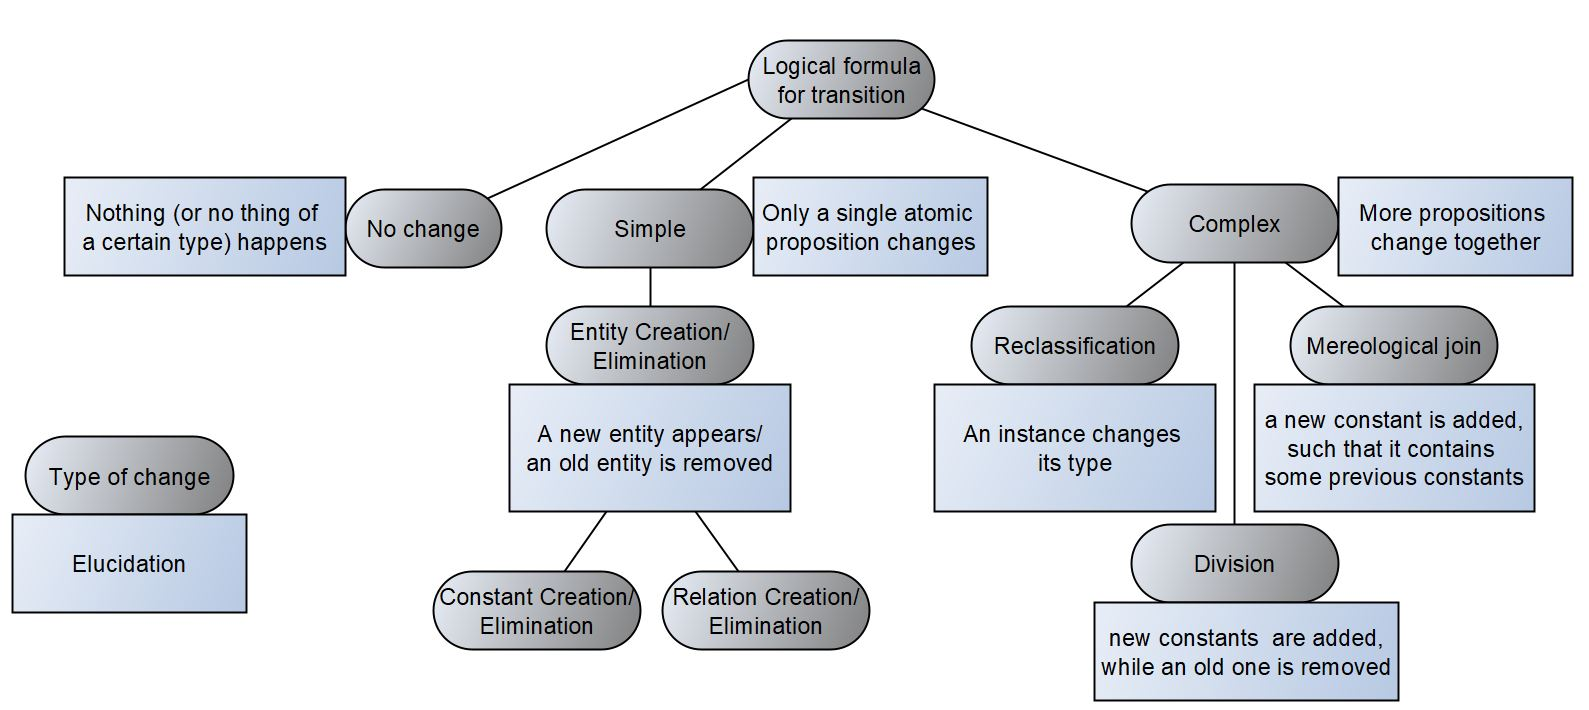
\includegraphics[width=\textwidth]{onto-func-logicv2.JPG}
  \caption{\label{fig:onto-func-logic} A non exhaustive taxonomy of the logical formulas describing changes between states, classified depending on what predicates differ between the initial and final states.}
\end{figure}
\begin{figure}
  \centering
  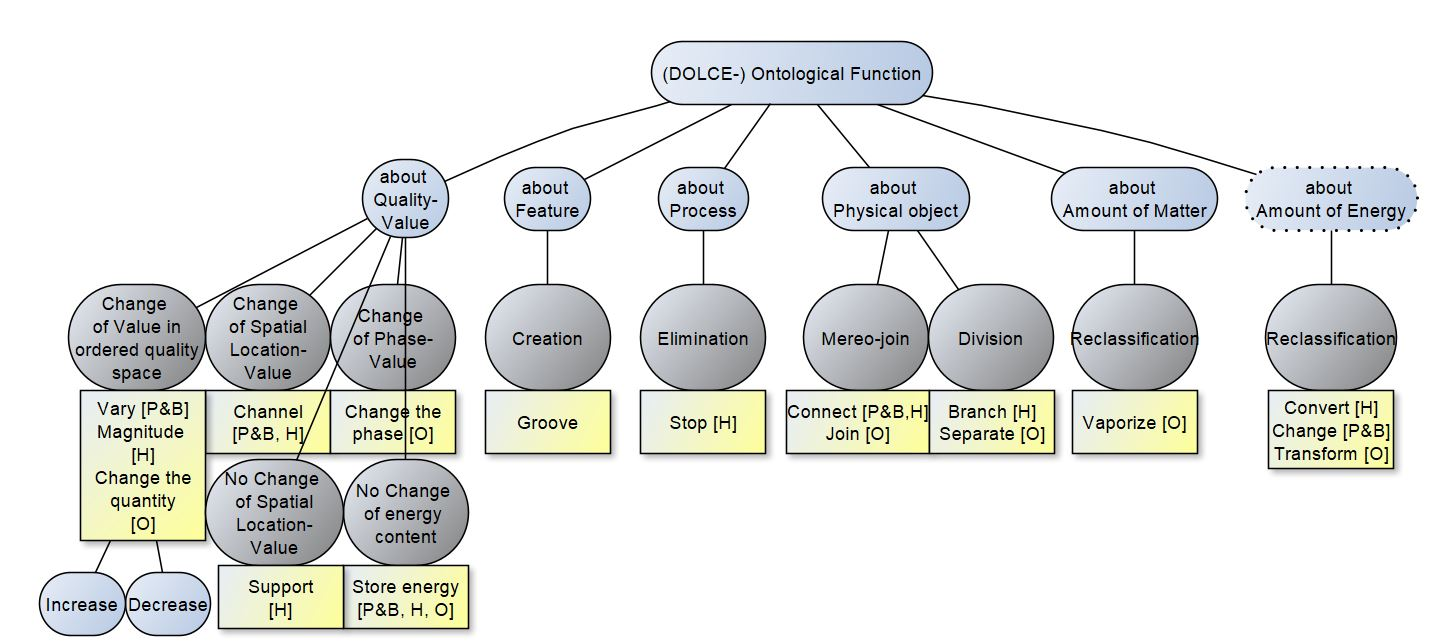
\includegraphics[width=\textwidth]{onto-func-taxav2.JPG}
  \caption{\label{fig:onto-func-taxa} A possible taxonomy of \ontoFunc{fullPlural}. The light blue rectangles contain the \ontoFunc{fullPlural}-categories. The gray circles contain the corresponding type of change at a logical level, and refer to Figure \ref{fig:onto-func-logic}. Finally, the yellow rectangles contain terms used by other authors that could, arguably, used to label the \ontoFunc{fullSingular} category: H, P\&B, and O refers to \cite{hirtz_functional_2002}, \cite{pahl_engineering_2007}, and \cite{sasajimaFBRLFunctionBehavior1995} respectively. Notice that some of these terms are used by their authors with different meaning than in this figure, additionally, we do not have added terms related with information content.}
\end{figure}
%%%

Note that an ontological category can be involved in a transition in different ways. 
For example, an instance of said category could be eliminated, meaning that the instance was present in the state before the transition but not after, or an instance could be created, meaning that the instance was not present before a transition but only after.
Another possibility is that there is a change of a relation of the ontology, e.g., in the initial state there were two individuals that were, say, one part of the other, while in the final state they are not.
More complex changes can be described, depending on the difference between the initial and final structure of the ontology. Note also that in most cases the same event may be classified by several \ontoFunc{fullPlural}. For instance, an event of cutting by a device, say a knife, is also a squeezing event, i.e., a compression (a change of the shape quality of the initial object) and a moving event (a change of the device location relatively to the object's location).\TODO{S: ho aggiunto questo esempio di un evento classificato da più funzioni. [FC:ok]}
%, thought of as a knowledge base\footnote{The changes are, therefore, relative only to the Abox of the knowledge base.}.
We have reported some of these cases in Figure \ref{fig:onto-func-logic}, which is not exhaustive.
\myComment{Notice that the classification discussed in this paragraph is only at a logical level, and must be joined with an ontological classification to find terms that are typical of the natural language.}
Finally, the functional terminology used in this paragraph is  inspired by engineering literature which, as we have seen earlier, is not homogeneous. 
For instance, the \firstTimeKeyWord{reclassification} (i.e., a change such that an instance changes type) of energy or matter is in other places called \quotes{convert} \cite{hirtz_functional_2002, sasajimaFBRLFunctionBehavior1995} or \quotes{change} \cite{pahl_engineering_2007} or \quotes{transform} \cite{kitamuraOntologybasedSystematizationFunctional2004}, while the change of value of a spatial location quality is called \quotes{channel} \cite{pahl_engineering_2007,hirtz_functional_2002}, and so on.

\myComment{Notice that some}
Functional terms that are linked to domain-level terms (e.g., \quotes{vaporize}, \quotes{moisten}, \quotes{heat})
are not captured at the lever of \ontoFunc{fullPlural} and require a domain or middle-level ontology containing corresponding concepts (e.g., vapour, humidity, temperature) in order to expand the construction we have just described up to that level of ontological distinctions.
\myComment{Unfortunately, there are terms that are commonly used in engineering and physics, but are difficult to describe ontologically.} 
%For example, \quotes{energy} and \quotes{signal}. 
The ontological nature of some concepts, like \quotes{energy},
\myComment{\footnote{Another notable example is \quotes{information}.}, its ontological nature} 
is unclear \cite{mcginnOntologyEnergy2012} despite being a fundamental concept in engineering and physics. 
\myComment{In this paper, we are not interested in discussing what energy is, only in showing that,} 
Nonetheless, given an ontology containing a conceptualisation of energy, it is possible to introduce a corresponding \ontoFunc{fullSingular}, which might be different in another ontology with a different conceptualisation of energy.
For instance, one could conceptualize energy as a quality, as done in~ \cite{borgoFormalizationFunctionsOperations2011}. 
This is the case, arguably, when one speaks about the energy \textit{of something}, e.g, of a battery.
In this case, in our ontology there would be a, say, \textit{energy content} quality-type, which gives rise to a corresponding \textit{convert energy} ontological function.
Another possibility is to conceptualize energy as an endurant, which can reside into entities, change its location, and change type (e.g., heat energy, kinetic energy, etc.).
In that case, the \textit{convert energy} ontological function would be a reclassification-type transformation.
%The point is that natural language is ambiguous, and making terms refer to a formal ontology necessarily disambiguates them, so that the same natural language term could be used to label many predicates defined using said ontology.\todo{S: l'ambiguità del NL non mi sembra interessante in una discussione delle funzioni ontologiche.}

Formalizing \myComment{this intuition that we have described about} \ontoFunc{fullPlural} might be difficult. One would benefit from the introduction in the ontology of a general relation `change of \ldots in event \ldots'.
An ontological function, as understood in this paper, is essentially an event classifier which looks at what changes (or remains stable) in the event. 
\myComment{A possibility is defining \ontoFunc{fullPlural}-types by making them classify those events such that there is a given relation between the situation at the initial instant and at the final instant of the event.
For instance,} 
This suggests defining specific functions by comparing, for instance, initial and final states. For example, a \textit{connect} function could be introduced as follows:
\bflist
  \item[\mydf{connect}] $ \Connect{x} \myiff (\DOLCECLbyBinary{y}{x} \myiff \DOLCEEvent{y} \land \sState{y}{s_i}{t_i} \land \eState{y}{s_f}{t_f} \land \Goal{s_f} \land \exists a,b,c (\DOLCEPhysObj{a} \land \DOLCEPhysObj{b} \land \DOLCEPhysObj{c} \land \DOLCEPC{a}{s_i}{t_i} \land \DOLCEPC{a}{s_f}{t_f} \land \DOLCEPC{b}{s_i}{t_i} \land \DOLCEPC{b}{s_f}{t_f} \land %\exists c (
  \DOLCEPC{c}{s_f}{t_f} \land \DOLCEPart{a}{c}{t_f} \land \DOLCEPart{b}{c}{t_f}) \land \neg \exists c' (\DOLCEPhysObj{c'} \land \DOLCEPC{c'}{s_i}{t_i} \land \DOLCEPart{a}{c'}{t_i} \land \DOLCEPart{b}{c'}{t_i})) $ \TODO{S: ho cambiato limitando a ph. obj., controlla [FC: ok, controllato]}
  \myComment{\item[] \mytext{A concept is of \textit{connect} type if and only if it classifies precisely those events that are transitions between a starting state ($s_i$, with time extension $t_i$) and a final state ($s_f$, with extension $t_f$) and, moreover, there are two entities ($a$ and $b$) that participate in such states and, during the final state but not in the initial one, form a single object ($c$)}}
    \item[] \mytext{A concept is of \textit{connect} type if and only if it classifies precisely those events that are transitions between a starting state ($s_i$, with time extension $t_i$) and a final state ($s_f$, with extension $t_f$) and, moreover, there are two physical objects ($a$ and $b$) that participate in such states and, during the final state but not in the initial one, they are both part of a physical object ($c$)}\TODO{S: aggiustato di consequenza [FC:ok]}
\eflist 
In the previous formula we used the predicate $\sState{y}{s_i}{t_i}$ to mean that $s_i$ is a state with time extension $t_i$, which is part of the perdurant $y$ and such that there are no parts of the time extension of $y$ which precede $t_i$. Analogous meaning for $\eState{\cdot}{\cdot}{\cdot}$.
Notice that: $(a)$ this notion captures the act of forming a single object out of two given ones, to formalize an assembly function one should add the condition that the final object is also a single piece (self-connected); $(b)$ if one reverses the initial and final states in Formula \refdf{def:connect}, then one obtains a definition for the \textit{divide} function.\marginpar{\color{red}{ho aggiunto}}

%%Moreover, notice that \refdf{def:connect} is not teleological by itself

Another example, to define a \textit{convert} function: 
\bflist
  \item[\mydf{convert}] $ \Convert{x} \myiff (\DOLCECLbyBinary{y}{x} \myiff \DOLCEEvent{y} \land \sState{y}{s_i}{t_i} \land \eState{y}{s_f}{t_f} \land \Goal{s_f} \land \exists \Phi,\Psi,a (\Phi\in\mathcal{NR} \land \Psi\in\mathcal{NR} \land \Psi\cap\Phi = \emptyset \land  \DOLCEPC{a}{s_i}{t_i} \land \DOLCEPC{a}{s_f}{t_f} \land \Phi(a,t_i) \land \Psi(a,t_f))) $ 
  \item[] \mytext{A concept is of \textit{convert} type if and only if it classifies precisely those events that are transitions between a starting state ($s_i$, with time extension $t_i$) and a final state ($s_f$, with extension $t_f$) and, moreover, there is an entity ($a$) that at time $t_i$ is instance of a type ($\Phi$), while at time $t_f$ is instance of a different, disjoint, type ($\Psi$). Necessarily, $\Phi$ and $\Psi$ are types belonging to the set of all non-rigid types of the underlying ontology ($\mathcal{NR}$)}
\eflist 
Notice that in the previous definition we have quantified over the set of all non-rigid classes of an ontology ($\mathcal{NR}$). 
If such a set is finite, like in \DOLCE, then the quantification corresponds to a finite disjunction of predicates, therefore Formula \refdf{def:convert} is a first-order formula.
Moreover, upper-level ontologies typically contain only rigid categories (e.g., if an individual is a physical object, it is always a physical object), therefore, such a convert function becomes useful when modelling changes in entities that go through phases \cite{guarinoOverviewOntoClean2009}, when modelling entities that change their processual role (as described earlier) or in combination with non-rigid categories (as provided by middle or domain-level ontologies).

%%%
The type of all \ontoFunc{fullPlural} that involve some change in quality values could be defined as follows:
\bflist
  \item[\mydf{changeQualityValue}] $ \ChangeQualityValue{x} \myiff (\DOLCECLbyBinary{y}{x} \myiff \DOLCEEvent{y} \land \sState{y}{s_i}{t_i} \land \eState{y}{s_f}{t_f} \land \Goal{s_f} \land \exists a,q,v_i,v_f (\DOLCEQualityDirect{q}{a}{t_i} \land \DOLCEQualityDirect{q}{a}{t_f} \land v_i \neq v_f \land \DOLCEPC{a}{s_i}{t_i} \land \DOLCEPC{a}{s_f}{t_f} \land \DOLCEQualeTer{q}{v_i}{t_i} \land \DOLCEQualeTer{q}{v_f}{t_f})) $ 
  \item[] \mytext{A concept is of \textit{change of quality-value} type if and only if it classifies precisely those events that are transitions between a starting state ($s_i$, with time extension $t_i$) and a desired final state ($s_f$, with extension $t_f$) and, moreover, there is a participating entity ($a$) which has a quality ($q$) with different values, $v_i$ and $v_f$, at times  $t_i$ and $t_f$, respectively.}
\eflist
If the case that the quality appearing in the formula \refdf{def:changeQualityValue} is of type spatial location, the ensuing \ontoFunc{fullSingular} will be of type \textit{channel}.
Instead, if the quality in \refdf{def:changeQualityValue} is such that it takes values into an ordered space (e.g., \textit{temperature}, \textit{humidity}, etc.) then the ensuing \ontoFunc{fullSingular} will be of type \textit{vary}, which can clearly be specialized into \textit{increase} and \textit{decrease} types. (We are borrowing this engineering terminology primarily from \cite{hirtz_functional_2002} and \cite{pahl_engineering_2007}.) 
%%%
Some functions, such as \textit{store} and \textit{support}, hint at the absence of change, as, for instance, a battery stores energy very well if it does not lose its charge over time, while a load-bearing wall supports the roof only if the roof does not fall. 
Therefore, concepts like store, support, or similar terms could be defined by modifying formula \refdf{def:changeQualityValue} imposing that the initial and final values of the quality are equal (relatively to the features of interest) instead of different.
%%%

At this point we make three observations: 
\begin{itemize}
  \item first, some processes are impossible to categorize only by observing the differences between a single couple of states.
  Take, for example, a temperature-controlled oven. 
  The controller unit of the oven makes it so that the temperature in the oven stays, up to some tolerance, at a target value.
  The controller could achieve this by turning off the heat when a sensor realizes that the target value is surpassed, and by turning on the heat when the current temperature is less than the target. 
  This makes it so that the temperature value over time oscillates around the target value (because the temperature keeps overshooting or undershooting), and such a process cannot be deduced by only observing the differences between two states.
  Therefore, processes like this cannot be reduced to \ontoFunc{fullSingular}.
  In this particular case, one could also argue that the function of the controller is to maintain the temperature in the oven around the set temperature\footnote{This could be expressed in the style of the previous definitions by comparing an initial state, in which the set value and the actual value are different, to a final state, in which said values are equal.}, while the oscillations of the temperature are merely a side effect of the chosen implementation method, and would be different, or even absent, if the implementation method was different. 
  In general, though, if one actually wishes to classify a transformation that cannot be described by comparison of two states, then the method employed in the previous formulas is not sufficient and a suitable comparison of what happens {\em during} the event should be added. We do not investigate this situation further but recall that, to maintain the overall view, one should add only conditions that are expressible within the language of the ontology.\marginpar{\color{red}{aggiunto frase}}
  \item Second, actual events can be extremely complex and participated by many relevant entities (think, e.g., the complexity of waking from a biomechanical point of view). 
  This, together with the fact that we admit also \ontoFunc{fullPlural} defined by the absence of some type of change (e.g., \textit{support}), makes so that many events would be classified by a combination of \ontoFunc{fullPlural} (as observed earlier while discussing the cutting example).
  This is not unexpected, and, in fact, reflects the flexibility of teleological thinking.
  Take, for example, a load-bearing wall.
  One could say that its function is to \textit{support} the weight of the roof, but it may also \textit{transmit} the load to the floor, or even \textit{stop} the wind from entering the house, or \textit{divide} the space inside the house into smaller rooms, and so on. 
  To recognize what aspect is the most relevant in a given context is a task for the engineer or technician, which, using their contextual view and creativity, determine what aspects to focus on. This is the reason for using the term `function' (in combination with `ontological', a qualifier we justified earlier) to characterize these classifiers.
  Events, by their nature, are open to different interpretations. 
  \item Lastly, we argue in favour of the flexibility of \ontoFunc{fullPlural}.
  In the previous paragraphs, we have mainly used functional terms taken from the Functional Basis \cite{hirtz_functional_2002} or from the influential view of \cite{pahl_engineering_2007}.
  Such vocabularies are indeed capable of expressing a vast quantity, if not the totality, of functions used within engineering domains, but they may not do so in the most natural way.
  For example, suppose that one is working with tooling machines that cut holes, slots, grooves, etc. in the workpieces. 
  Then, using the Functional Basis one is reduced to using just the term \textit{remove} to talk about the functions realizing such features in the workpiece.
  Instead, if one uses a domain ontology that contains concepts such as hole, slot, groove, etc., then one can build corresponding functional terms, say \textit{make hole}, \textit{make slot}, \textit{to groove}, etc., defined analogously to the previous formulas.
  Such terms may be more natural than just using \quotes{removing}, and may even differ significantly  from \quotes{removing}, depending on their precise formalisation.
  Another example: in the Functional Basis vocabulary, the term \quotes{stop} means \quotes{to cease the transfer of a flow}, for instance \quotes{A reflective coating on a window stops the transmission of UV radiation through a window} \cite{hirtz_functional_2002}. But what if perdurants are important in our domain and we want to say that something \textit{stops a process} (e.g., \qquotes{The addition of a respiratory inhibitor stops the absorption of amino acids}, not that \qquotes{stops the amino acid-material-flow from moving}, but that it \qquotes{stops the absorption}, where absorption is an important element of the domain?
  %Altro esempio: camiamento di stato come camiamento di *stato* o cambiamento di *stato di aggregazione*
  We could derive useful functional terms, from an appropriate domain ontology managing concepts of domain processes.
\end{itemize}
%%%

%%%
Up to this point we have defined some types of \ontoFunc{fullPlural}, but not the concept of \ontoFunc{fullSingular} itself. 
A possibility is to find an exhaustive list of types of \ontoFunc{fullPlural} and then define \ontoFunc{fullSingular} as the disjunction of all those types, for instance:
\bflist
  \item[\mydf{ontoDef1}] $ \FunctionAbs{x} \myiff (\Connect{x} \lor \Divide{x} \lor \Convert{x} \lor \dots) $
\eflist
%This is, in principle, correct, but, in practice, requires an exhaustive enumeration of top-function types, which we do not want to commit to, in this paper. 
This can be done by providing an exhaustive list of ontological functions made available by an upper ontology.
Another possibility is to look for an intrinsic definition of \ontoFunc{fullPlural} that informally could be as follows:
\bflist
  \item[\mydf{ontoDef2}] \mytext{A concept is a \ontoFunc{fullSingular} if and only if it classifies exactly those events consisting in a transition \myComment{from an initial state to a final state} such that the changes (or the absence thereof) between the initial and final states (or across the whole transition) is characterized in terms of a formula expressed in the language of an upper ontology.}\TODO{S: ho esteso il significato perché l'espressione era limitante [FC:ok]}
\eflist
%(Of course, the formulas that engineers actually use to express functions are not so broad as in \refdf{def:ontoDef2}, and typically focus on a small set of cases).
Since \qquotes{a formula expressed in the language of an upper ontology} is not something that can be written in a natural way using first-order logic, we cannot give an intrinsic first-logical definition of \ontoFunc{fullPlural}. (A similar argument could be applied to extend the notion of ontological functions to functions in the language of reference ontologies.)\marginpar{\color{red}{ho separato i casi upper e reference.}}


\paragraph[meta]{Link between systemic functions and \ontoFunc{fullPlural}.}
Returning to the relation between systemic functions and \ontoFunc{fullPlural}, we observe that the former correspond to system-dependent functional descriptions, while the latter corresponds to system-independent functional descriptions. 
Since \ontoFunc{fullPlural} are more general than systemic functions, they can be used to classify them:
%% DA SOPRA-->The informal intuition of \ontoFunc{fullPlural} is that they are classified according to the ontological change they realize between the input and the output states. In this sense, they are independent of systemic functions. Yet, every systemic function is associated to one or more \ontoFunc{fullPlural}, depending on the changes it classifies. 
%of the  the following relation between \ontoFunc{fullPlural} and systemic functions holds:
\bflist
 \item[\myax{functionAbstr}] \myComment{$ \FunctionAbs{x} \myfi (\DOLCEConcept{x} \land \exists y,t (\DOLCECLby{y}{x}{t}) \land \forall y,t (\DOLCECLby{y}{x}{t} \to \FunctionSys{y}) $}
 $ \FunctionAbs{x} \myfi (\exists y ( \DOLCEConceptSubsum{y}{x} \land \FunctionSys{y}) \land \forall y (\DOLCEConceptSubsum{y}{x} \land \neg \FunctionAbs{y} \myfi \FunctionSys{y})) $
 \item \mytext{any \ontoFunc{fullSingular} $x$ is specialized by some systemic function $y$ and, beside \ontoFunc{fullPlural}, classifies systemic functions only.}
\eflist
For example, take a tooling machine as a system, e.g., a lathe, and assume that it makes use of two electrical motors: one for rotating the spindle and %one 
the other for moving the spindle horizontally. %Then, 
Both electrical motors perform the same \ontoFunc{fullSingular} of \quotes{converting} (electrical energy into mechanical energy), but they also perform two different systemic functions %that 
specializing the \ontoFunc{fullSingular} in the context of the lathe: \quotes{converting (electrical energy into mechanical energy) to rotate the spindle}, and \quotes{converting (electrical energy into mechanical energy) to translate the spindle}, respectively.
The intuition is that we can group systemic functions together through common characteristics, along the lines of definitions \refdf{def:connect} to \refdf{def:changeQualityValue}, abstracting from specific systems or from their occurrences in different parts of the same system.

%Such ontologically functions reflect a perdurant taxonomy based on functional grounds, meaning that a given taxonomy of perdurants corresponds to a taxonomy of functions as given in \cite{borgoKnowledgebasedAdaptiveAgents2019}. TODO:<--reinserire-->
%
%, by stating that functions of some type must be played only by perdurants of the corresponding type. 
%As said, we obtain the types of \ontoFunc{fullPlural} using the variation of some condition before and after the realisation of the function. For example, it is common to speak of `connect' or `change' functions \cite{pahl_engineering_2007}, that is, of functions whose underlying perdurant is such that the number of operands or, respectively, the operand type is modified during the event. Similarly, other ontological  functions-types could be obtained considering variation of other properties, as done in \cite{borgoCapabilitiesCapacitiesFunctionalities2021} and \cite{borgoKnowledgebasedAdaptiveAgents2019}, or specializing existing \ontoFunc{fullPlural} to special cases, e.g. specialize `change' to `change electrical energy into torque'.
%In this paper, we do not characterize further the taxonomy of \ontoFunc{fullPlural}, nor discuss the organisation of their taxonomy beyond what presented in \cite{borgoKnowledgebasedAdaptiveAgents2019}. 

Finally, notice that the two types of functions introduced in this paragraph cover at least two different ideas of functions used by engineers. 
First, there are \quotes{general} functions that engineers use when they need to, say, describe information about or collect information from different systems. For example, Collins \cite{collinsFailureExperienceMatrixUseful1976}, when collecting and analyzing failure experience data, speaks of \quotes{elemental mechanical functions}, which are application-independent characterisations of \quotes{basic} functions. %\quotes{distinctive generic characterisation of the basic function of a machine part without reference to the specific application for which it is used} 
Analogously, Pahl et Beitz \cite{pahl_engineering_2007} speak of \quotes{generally valid functions}, and propose them as  references for cataloguing design knowledge about function implementation. 
These types of functions can be approximated via \ontoFunc{fullPlural}.
In contrast, a second meaning used by engineers is system-dependent. In general, when engineers focus on a single system, they use different concepts to speak about the system components. The terminology is varied, but typical terms are `serial number', that is the identifier of a component-instance, `component code', i.e. the component or assembly-type identifier, and `functional location' or `tag', which are identifiers that consider also the position of a component within a system. For example, Figure \ref{fig:hydroSystem} schematises a hydraulic system containing four solenoid valves, whose tags are EPF1 to EPF4. These tags cannot refer to the valve-type, since the four valves could have the same type, nor they can refer to the valve-instances, since schema are generally used to represent different system-instances. 
\begin{figure}
  \centering
  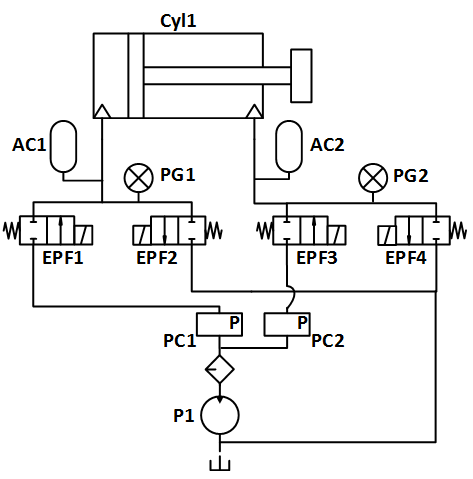
\includegraphics[width=0.45\textwidth]{imamoTAXA.PNG}
  \caption{The scheme of some hydraulic system, taken from \cite{HydroPNG}.  \label{fig:hydroSystem}}
\end{figure}
In our terminology, we could say that tags identify roles that components play in a system. Necessarily, these roles are of functional nature, for each component in an engineering system has a role in the system function. Thus, tags or, at least, the teleological content they carry, could be formalized by systemic functions. %Indeed, tags should carry also information about, say, the structural links of the underlying component with the remaining components of the systems. 
%\TODOinline{[SB: manca un risultato conclusivo che giustifichi perché ci fermiamo qui. bisogna dare almeno qualche indicazione di quali concetti di funzione usati in ingegneria cadono sotto questo approccio (nel senso che possono essere considerate specializzazioni di queste definizioni)][ Ho provato a inserire un paragrafo argomentando che le "generally valid functions" di Pahl e Beitz assomigliano alle funz.ont. e che i tag/sigle/functional location assomigliano alle fun.sys.]*[SB: ok, per ora va bene. magari in fase di revisione vediamo se riusciamo ad approfondire questo punto][FC:ok][S: complessivamente la discussione ora va bene :-)}
%\textcolor{blue}{(se capisco, le \ontoFunc{fullSingular} sono ruoli giocati dai perdurant. E qst perdurant sono i behaviour degli artefatti/sistemi che hanno come scopo la realizzazione di un certo goal.  Per aiutare i lettori, sottolinerei nel testo che la nozione di \ontoFunc{fullSingular} e' un ruolo/concetto (forse ho perso qst informazione))(FC: è sotto la definizione di funz. sys., ma per sicurezza ho aggiunto anche all'inizio di sottosezione)}



\subsection{Functional decomposition}\label{subsec:fun-dec}
An important feature of functions in engineering is the possibility to decompose them into sub-functions. This also allows to refine the granularity of the system description. In this paragraph, we show how such decomposition relation can be used in order to formalize the difference between \ontoFunc{fullPlural} and engineering functions that we described earlier.

First, observe that such decomposition cannot be reduced to a partial order relation between functions.  
That is, if we represent the functional decomposition of a function, say $\cst{f}$, into sub-functions, say $\cst{f}_1, \cst{f}_2, \dots, \cst{f}_n$, as $\decom(\cst{f};\cst{f}_1,\cst{f}_2,\dots,\cst{f}_n)$, then it does not seem possible to find a parthood relation such that $\decom$ reduces the mereological sum.
This is caused by, at least, the following reasons:
\begin{itemize}
  \item Functions exist at a teleological level, therefore, any decomposition of functions must take into account the decomposition of the underlying objective substrata, that is, of the underlying behaviours and objects.
  \item The sub-functions of a function must `organize'\footnote{We borrow the term from Vermaas and Garbacz \cite{vermaasFunctionalDecompositionMereology2009a}, in there the interested reader can find a discussion about mereology in functional decomposition, especially with respect to the Functional Basis methodology.} in order to realize the decomposed function. In particular, the composition of a mere set of functions is not unique.
  \item The same function can be decomposed in more ways, therefore the decomposition relation is of type many-to-many.
  \item Not all combinations of sub-functions are possible, due to physical and technical constraints. 
  Moreover, among all possible combinations, engineers recognize typical ones and use them systematically. 
\end{itemize}
Additionally, Vermaas has proven that attempting to model a Functional Basis style of functional decomposition\footnote{That is, a style where functional models can be graphically represented as directed graphs with flows as edges and function as nodes. The composition, then, can be in series, between nodes that share an edge (canceling that edge), or in parallel, between nodes that do not share edges.} entails contradictions \cite{vermaasFormalImpossibilityAnalysing2013}\footnote{The counterexamples shown are based on some additional assumptions. Precisely that, first, if a function-token is part of another function-token, then the same holds for the corresponding types; and, second, that flow loops are possible. %(note that the presence of loops, entails that some functions compose into a null-token).
}, so that there are also formal obstacles preventing the application of classical mereology to functional decompositions.
We do not attempt a solution to these problems here,
%\footnote{%\TODO{will we do it in the future? [SB: lasciamo stare questo per ora]}}, 
instead we assume that the relation $\decom$ is given, and focus on engineering \methodsName{plural}. 

Inspired by the work of Kitamura et al. on `ways of functional achievement' \cite{kitamuraOntologicalModelDevice2006, kitamuraOntologybasedDescriptionFunctional2003}, we consider engineering \methodsName{plural} as \methodsDefinition{plural} representing the knowledge that engineers share about ways of implementing functions through functional decomposition:
\bflist
  \item[\myax{methodSubs}] $ \Method{x} \myfi \DOLCENASO{x}$ %\TODOinline{[SB: dopo le variazioni questo è l'unico posto dove parliamo di descrizioni e non mi sembra neppure rilevante. visto che qui il metodo è solo informazione per la functional decomposition, potremmo chiamarlo wayOfAchievement e usarlo come relazione: data una main-function f, $wayOfAchievement(f,f_i)$ vale se $f_i$ è una sottofunzione][FC: non è possibile, perche' la relazione 1-a-molti verrebe persa. Comunque ho optato per trasformare i 'methods' in anonimi social objects che non quantificano. Comunque, eventuali modifiche sarebbero veloci. Se, ad esempio, decidiamo di cambiare il nome 'method', ho già realizzato un apposito comando (methodsName). Se decidiamo di cambiare la categoria di DOLCE a cui appartengono basta cambiarla qui e, per la terminologia, nell'appositio comando (methodsDefinition)]*[SB: non capisco, la relazione $wayOfAchievement(f,f_i)$ è 1-a-molti, vale per tutte le coppie $(f,f_i)$ dove la seconda è una sottofunzione, quello che si perde è eventualmente l'ordine di esecuzione][FC: sì, scusa, hai ragione, mi sono espresso male. Sicuramente si perde l'ordine di esecuzione, però si perdono anche gli 'insiemi' di decomposizione. Cioè, supponi che, usando il primo formalismo, abbiamo decomp(F;f1,f2) e decomp(F;f3,f4). Allora, usando il secondo formalismo abbiamo wayOfA.(F,f1), wayOfA.(F,f2), wayOfA.(F,f3), wayOfA.(F,f4); che però poteva essere derivato anche da decomp(F;f1,f2,f3,f4)]} 
\eflist
Formally, such \methodsDefinition{plural} can be understood as reifications of functional decomposition relations.
Precisely, we introduce roles $\mainFunctionRole{\cdot}$ and $\subFunctionRole{\cdot}$, contextualized by a decomposition, such that:
\bflist
  \item[\myax{main-sub-functions-sussum}] $ (\mainFunctionRole{x} \lor \subFunctionRole{x}) \myfi (\DOLCERole{x} \land \exists \cst{m} ~(\Method{x}  \land \founded{x}{\cst{m}}))$
  \item[] \mytext{main-functions and sub-functions are roles founded on some engineering \methodsName{singular}}
\eflist 
Additionally, we assume that \methodsName{plural} are always contexts for a main-function and for a certain number of  sub-functions (axiom \refax{ax:pre-pre-method}$^*$ is actually a meta-axiom, for this reason we mark it with a $*$-symbol). 
\bflist
  \item[\myax{pre-pre-method}$^*$] $ \Method{\cst{m}} \myiff \exists! n ~\MethodBin{\cst{m}}{n},$ and $n$ is integer
  \item \mytext{Each method, say $\cst{m}$, has a (unique) number, say $n$, of  sub-functions that are contextualized by the method}
\eflist
Note that, given a finite set of methods, the previous axiom can be substituted with a finite set of axioms in FOL. The following condition constrains the decomposition relationship and is expressed via an axiom schema (here $n$ is an integer):\TODO{S: vedi se ti torna la prima osservazione, infatti l'assioma messo così assume che usiamo il modello standard degli interi che non è assiomatizzabile [FC: sì. Infatti a14+a15 di fatto servono per scrivere uno schema di assiomi in modo carino, e "and $n$ is an integer" sta fuori dalla teoria propria]}
\bflist
  \item[\myax{pre-method}$^{schema}$] $ \MethodBin{\cst{m}}{n} \myfi \exists!  \cst{main}, \cst{sub_1}, \ldots, \cst{sub_n} (\mainFunctionRole{\cst{main}} \land \subFunctionRole{\cst{sub_1}} \land \ldots \land \subFunctionRole{{\cst{sub_n}}} \land \founded{\cst{main}}{\cst{m}} \land \founded{\cst{sub_1}}{\cst{m}} \land \ldots \land \founded{\cst{sub_n}}{\cst{m}}) $
  \item[] \mytext{for any engineering \methodsName{singular} of functional decomposition, say $\cst{m}$, having a given number of sub-functions, say $n$, there exist a main-function role and $n$ sub-function roles, which are founded on $\cst{m}$ and are uniquely determined}
\eflist
Since the main-function and the $n$ sub-functions roles of a given \methodsName{singular} are univocally determined, we can represent them with functional symbols. In particular, we will write $\cst{main^m}$, $\cst{sub}^m_1$, \dots, $\cst{sub}^m_n$ to indicate the roles corresponding to the \methodsName{singular} $\cst{m}$, as per Axiom \refax{ax:pre-method} (we omit the functional dependence of $n$ on $\cst{m}$, for ease of notation).
\myComment{Then, we define two binary relation that we will use as shortcuts to simplify the incoming definition schema \refdf{def:method}
\bflist
  \item[\mydf{main-function-of}] $ \mainFunction{x}{\cst{m}} \myiff \DOLCECLbyBinary{\cst{f}}{\cst{main}^{\cst{m}}} $
  \item \mytext{$x$ is main-function-of a method $\cst{m}$ if and only if it is constantly classified by the main-function role corresponding to $\cst{m}$} 
  \item[\mydf{sub-function-of}] $ \subFunction{x}{\cst{m}} \myiff \DOLCECLbyBinary{\cst{f}}{\cst{sub}^{\cst{m}}_i} $
  \item \mytext{$x$ is main-function-of a \methodsName{singular} $\cst{m}$ if and only if it is constantly classified by the any of the sub-function roles corresponding to $\cst{m}$} 
\eflist}
Finally, the link between \methodsName{plural} and decompositions is given in the following definition schema: 
\bflist
  \item[\mydf{method}$_{schema}$] $\decom(\cst{f};\cst{f}_1,\cst{f}_2,\dots,\cst{f}_n) \myiff \\ ( \FunctionSys{\cst{f}} \land \FunctionSys{\cst{f}_1} \land \ldots \land \FunctionSys{\cst{f}_n} \land \\ \exists \cst{m} (\Method{\cst{m}} \land \DOLCEConceptSubsum{\cst{f}}{\cst{main}^{\cst{m}}} \land \DOLCEConceptSubsum{\cst{f}_1}{\cst{sub}^{\cst{m}}_1} \land \ldots \land \DOLCEConceptSubsum{\cst{f_n}}{\cst{sub}^{\cst{m}}_n}) $
 \item \mytext{$\cst{f}$ is decomposed in $\cst{f_1},\ldots,\cst{f_n}$ if and only if they are all systemic functions and there is a \methodsName{singular} with corresponding main-function $\cst{main}^{\cst{m}}$ and sub-functions $\cst{sub}^{\cst{m}}_1$, \dots, $\cst{sub}^{\cst{m}}_n$, which are specialized by $\cst{f}$ and $\cst{f_1},\ldots,\cst{f_n}$, respectively}
\eflist

The advantage of this approach is manyfold: it makes possible to organize the \methodsName{singular}-types within sumbsumption taxonomies, for example, `spot welding' is a specialisation of the \methodsName{singular} `welding', which itself is an implementation \methodsName{singular} of the function `to join'; 
and to describe the properties of the \methodsName{plural}, for instance the working principle, say Kirchhoff's law for a `voltage divider' \methodsName{singular}. %, similarly to what has been done by Kitamura's team in  \cite{kitamuraOntologybasedDescriptionFunctional2003}.
Additionally, it makes possible to introduce properties of functional decomposition. For example, if one wishes to express that all functions are decomposable, she can state:
\bflist
\item[\myex{noAtomsFunctions}] $\FunctionSys{x} \myfi \exists y~ \mainFunctionRole{y} \land \DOLCEConceptSubsum{x}{y} \land x\neq y$ %\TODO{FC: why should this axiom be enforced? It implies no functional atoms. *[SB: è un commento per me? mi sono perso il contesto...][FC: avevi scritto che mi ero dimenticato questo assioma. L'avevi scritto vicino a \refdf{def:engfunction}.]*[SB: non ricordo bene. credo che l'idea venisse dal lavoro con Riichiro dove un sistema è sempre composto di almeno due parti e quindi decomponibile, ne segue che una funzione systemica è decomponibile (nei casi limite una delle due non "fa nulla", cioè è una funzie di mantenimento)][FC: ok, allora io o lascerei così]*[SB: ok]}
\eflist
Instead, if one wishes to state that a function, say $\cst{f}$, is not decomposable:
\bflist
\item[\myex{yesAtomsFunctions}] $\neg \exists y~(\mainFunctionRole{y} \land \DOLCEConceptSubsum{x}{y} \land x\neq y)$
\eflist
Moreover, this approach allows us to give a formal definition of engineering function and, thereby, to discuss the ontological difference between capacities and capabilities. 
In fact, we define engineering functions to be main functions
\bflist
  \item[\mydf{engfunction}]  $ \FunctionEng{x} \myiff \mainFunctionRole{x} $
  \item[] \mytext{engineering functions and main-functions coincide}
\eflist
so that engineering functions are roles that systemic functions, which are defined in \refdf{def:function}, can play in the context of a functional decomposition.
For instance, in the lathe example discussed above, it could be that the systemic functions of the two motors are both implemented through the \methodsName{singular} of, say, `three-phase electric motor', and, therefore, play the role of engineering functions. In this case, the functional decomposition  entailed by the \methodsName{singular} includes sub-functions roles for, say, `supply electrical energy' (one per each phase), `drive the motor', and `output mechanical energy'. 


%%%%%%%%%%%%%%%%%%%%%%%%%%%%%%%%%%%%%%%%%%%%
\section{Capabilities and capacities}\label{sec:CapabilAndCapac}
%%%%%%%%%%%%%%%%%%%%%%%%%%%%%%%%%%%%%%%%%%%%

In this section, we discuss capabilities and capacities, two notions that we briefly introduced at the end of Section~\ref{sec:review}. In particular, we will make use of the concept of  \ontoFunc{fullSingular} to distinguish capabilities from capacities. That is, we ground the distinction on an ontological argument moving beyond views like ISO 15531-31\cite{jochemISOISO15531312004}, which proposes the association of capacities with a quantitative viewpoint and capabilities with a qualitative viewpoint only on the basis of practical arguments.\marginpar{\color{red}{ho cambiato un po'}}
%\TODOinline{which, following the approach taken in ISO 15531-31\cite{jochemISOISO15531312004}, characterize the qualitative (capabilities) and the quantitative (capacities) viewpoints on what a device can do}.

%\myComment{Given that the difference between capabilities and capacities is expressed using the qualitative vs quantitative duality, a first idea is to model capacities as sublcasses of capabilities: for example, \cite{kochCAPABILITIESBASEDACCOUNTPATIENT2016} (despite not mentioning capacities) speaks of \qquotes{general and specific capabilities}, a general one being, for example, the \qquotes{capability of obtaining food}, and a corresponding specific capability being \qquotes{capability of obtaining through hunting whales on the sea for extended periods of time}. 
%Therefore, one could be tempted to say that there are no capacities at all, as an ontological category, but only more or less specific capabilities.
%This is a possible approach, but we argue against it, for (at least) two reasons: first, in engineering capabilities and capacities are often used as different concepts. Sometimes this difference is only implicit, sometimes it is explicit as in the ISO 15531.
%Secondly, some aspects of capabilities do not seem reducible to other, perhaps more specific, capabilities.
%Take, for example, Figure \ref{fig:capability-parameters}. 
%It shows two capabilities, \textit{moving} and \textit{finger grasping}, that a robot may have, together with some characterising parameters, such as \textit{paylod, workspace dimensions}, and so on. 
%It is possible that the parameter for workspace dimensions is linked to (or just is) a capacity quantifying the moving capability. In that case, it would be unnatural to call \quotes{workspace dimension} a capability, and, thus, the same should hold for capacities.%\TODO{FC: se quest'ultimo paragrafo non è convincente, rimuoverlo senza remore}.


%\begin{figure}
%  \centering
%  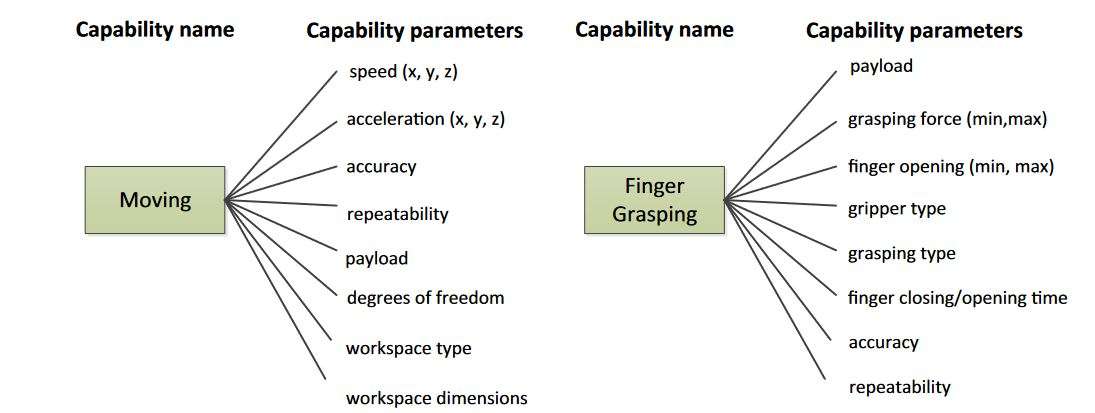
\includegraphics[width=\textwidth]{capability-parameters.JPG}
%  \caption{\label{fig:capability-parameters} Two possible capabilities of a robot and they respective parameters (taken from \cite{jarvenpaaDevelopmentOntologyDescribing2019a}).}%Capability parameters describe the characteristics of a capability.
%\end{figure}
%}

%In order to differentiate between capacities and capabilities, 
Recall that the characteristics of a technical artifact are part of its physical make-up and determine how the artifact interacts with its environment. 
For example, an individual pump is built in such a way that it is able to pump %hydraulic 
water with a certain flow rate.
Following the quality theory of \DOLCE, both the physical characteristics of the technical artifact and its `being able' to do something
%, that we shall call \firstTimeKeyWord{capabilities}, 
can be conceptualized as individual qualities.\footnote{As seen in Section \ref{sec:DOLCE}, individual qualities in \DOLCE have associated quality spaces, which are essentially types of conceptual spaces as introduced in \cite{Gardenfors2004}. In the case of capabilities, the associated quality spaces should characterize the kinds of entities through which the capability can be realized.} 
Consequently, we can model the capacity `flow rate' (something that can be quantified) as a relational quality of the artifact relative to a certain kind of fluid, and the capability to pump (something that realizes a type of interaction or ability) of the same artifact as another (yet related) relational quality.
But what are these capabilities? Our theory provides a natural explanation: an entity has a capability if it can participate as doer in an \ontoFunc{fullSingular}. More precisely, an entity has a capability of a certain type (it has the capability of dividing) if and only if it can participate in the role of doer in an \ontoFunc{fullSingular} of the corresponding type (it can participate as doer in a event classified by the divide function). Thus, we assume that \ontoFunc{fullPlural} define types of capabilities, and that an entity has a capability only if it can perform (participate as doer) the corresponding \ontoFunc{fullSingular}.\TODO{S: ho aggiunto questa parte per collegare capabilities e funz. ontologiche, secondo me va anticipata qui. [FC: ok]} Starting from this level of capabilities (which we could call ontological capabilities), one can specialize capabilities to lower functional levels where functions like cutting, loading etc. are introduced, thus characterizing cutting capability, loading capability and so on.\marginpar{\color{red}{aggiunto}}

\subsection{Capabilities vs. capacities}\marginpar{\color{red}{aggiunta sottosez.}}
Whenever a capability is based on some other quality of a technical artifact, that is, when each realisation of the capability depends on some other quality, we say that it is \firstTimeKeyWord{\foundedTerm{passive}} on that quality (or qualities). As before, we formalize this through the relation $\founded{\cdot}{\cdot}$ defined in \refdf{def:foundingBasic}.
For example, in the case of the pump we could say that the capability of the pump to move water is founded on its flow rate capacity.
%a person could say that he or she is able to jump high due to the strength of their leg muscles and their technical proficiency in jumping, that is, they have a jumping capability that is founded on their leg strength and their technical proficiency in jumping. 
Coming back to Gero and Qian's example of the water tap mentioned in Section \ref{sec:DOLCE}, which is similar to the one of the pump, we could say that the faucet has the capability of delivering water when requested, which is founded on its flow rate capacity, which is itself founded on its diameter quality (Gero and Qian say that the flow rate is \quotes{controlled} by the diameter \cite{qianFunctionBehaviorStructure1996}).
Now, in this example, there is a difference between the flow rate and the diameter: the latter is an intrinsic quality and the former is a relational quality, as we argued in Section \ref{sec:DOLCE}.
%Now, in this example, there is a difference between the leg strength and the jumping proficiency quality: the former is intrinsic and the latter is not, since it wouldn't exist without the jumping occurrences. 
%When \myComment{Whenever<-no: altrimenti sembra definizione} this happens, that is, \myComment{whenever} when a capability is founded on a relational quality, we call that quality \firstTimeKeyWord{capacity}, analogously to the approach in \cite{borgoCapabilitiesCapacitiesFunctionalities2021}. 
These examples suggest that  \firstTimeKeyWord{capacities} are those relational qualities on which a capability is founded, analogously to the approach in \cite{borgoCapabilitiesCapacitiesFunctionalities2021}. 
%and, analogously to \cite{borgoCapabilitiesCapacitiesFunctionalities2021}, we call the other qualities \firstTimeKeyWord{capacities}. 
The point is that capacities are relational qualities that provide information about how the corresponding capability can be realized in practice. 
Going back to the pumping example, we conclude that the flow rate capacity \myComment{quantifies} parametrizes, perhaps only partially, the pumping capability.  

Another example: electronic components such as resistors, transistors, etc., are accompanied by a datasheet that reports technical properties of the devices. 
Typical properties are, for example, the failure rate and the maximum temperature, current, or voltage that the component can reliably operate with in standard conditions. 
In our terminology, all the aforementioned properties are capacities: these properties are manifested only when the component is inserted into a working electrical circuit\footnote{As mentioned earlier in the paper, a clear-cut example is the voltage, which, since it is a potential, needs a fixed reference point in order to be measured.}; and they \myComment{quantify} parametrize some capability of the component like, say in the case of a resistor, to create a voltage drop. 

Capacities themselves are founded on some intrinsic physical qualities of the bearing object. For example, the maximum operating current will depend on the geometric and electrical properties of the conductor metal, such as its diameter and its resistivity. Similarly, the flow rate of the water tap depends on its diameter. Given these observations, we characterize capacities as follows:   
\bflist
\item[\myax{capacPartialDef}] $ \Capacity{x} \myfi \RelationalQuality{x} \land \exists y(\founded{x}{y} \land \IntrinsicQuality{y} \land \bearer{x} = \bearer{y}) $%(\DOLCEQualityDirect{y}{z} \land \DOLCEQualityDirect{x}{w} \myfi z = w)) $  % 
\item[] \mytext{A capacity is a relational quality and is founded on some intrinsic quality, which is carried by the same bearer.}%\TODOinline{[SB: se non è complicato farlo ora aggiungerei che x e y dovrebbero anche avere lo stesso bearer, altrimenti lasciamo per l'eventuale revisione][FC. hai sicuramente ragione, ma anche io lascerei a eventuale revisione][FC: aggiunto questo dettaglio]}
\eflist
In \refax{ax:capacPartialDef}, the $\bearer{\cdot}$ is the (unique) bearer of a quality, i.e.:
\bflist
\item[\mydf{beareDef}] $ \bearer{x} = \suchthat ~\! 
y (\DOLCEQualityDirect{x}{y}) $ 
\item[] \mytext{the bearer of a quality is the entity that has (inheres) the quality}\marginpar{\color{red}{aggiunto}}
\item[\myax{capacPartialDef2}] $ \Capacity{x} \myfi \exists y( \Capability{y} \land \founded{y}{x}) $  % 
\item[] \mytext{Each capacity founds a capability.}%\TODO{FC: ha senso questo assioma o è eccessivo (e in caso dire che hanno lo stesso bearer?)?}\TODO{S: per me va bene così}
\eflist
Axioms \refax{ax:capacPartialDef} and \refax{ax:capacPartialDef2} do not fully define what a capacity is. They only give some constraints.
\myComment{Since the classical case of deciding what relations there are between the color of an object and its hue is difficult (is the hue a quality of the color? Or maybe the hue is part of the color, or something else?)\TODO{FC:esiste citazione per questo?}\todo{S: non ne conosco, meglio tagliare questa osservazione, non è centrale}, }
Modelling the relation between capacities and capabilities remains complicated and requires further investigations. 
\myComment{In fact, one could even argue that color itself is a capability: the capability of reflecting certain lightwaves.}
%A full definition of capacity is, therefore, left as an open issue.
Yet, a promising way to tackle the problem
\myComment{among others, and the precise consequences of its adoption, with respect to other approaches, warrant further study.}
is to define a capacity as a \quotes{parameter} of the capabilities it founds, that is, as a quality such that its values are always related to the conceptual space of the corresponding capability:
 %(since this is only a suggestion, we mark this definition with a $\dag$-symbol):
\bflist
\item[\myex{capacFullDef}] $ \Capacity{x} \myiff \RelationalQuality{x} \land \exists y,z(\founded{x}{y} \land \IntrinsicQuality{y} \land \founded{z}{x} \land \Capability{z} \land \bearer{x} = \bearer{y} = \bearer{z} \land \forall u,t (\DOLCEQualeTer{u}{z}{t} \myfi \exists v (\DOLCEQualeTer{v}{y}{t} \land \DOLCEPart{v}{u}{t}))) $ 
\item[] \mytext{Capacities are precisely those relational qualities that are founded on some intrinsic quality (of the same bearer), and which found some capability (of the same bearer), such that every time that the capability takes a range-value ($u$), the capacity takes a value ($v$) which is part of $u$.}\TODO{S: visto che è solo un suggerimento, ho classificato questa def. come esempio. [FC:ok]}
\eflist
Briefly put, the formula above views capacities as the parameters of capabilities allowing to ontologically support practical approaches like, e.g., that of ISO 15531-31\cite{jochemISOISO15531312004}. 
\myComment{Our approach is to define a parameter as another quality whose values are mereological parts of the values of the original quality. }

\subsection{Capabilities vs. functions}\marginpar{\color{red}{aggiunta sottosez. ed eliminato il rif.to alla modalità}}
%In contrast to \refex{ex:capacFullDef}, a characterisation of capabilities may touch upon the fact that 
From another perspective, capabilities are inextricably intertwined to functional aspects. 
%In order to do this, we first try to clarify the nature of capabilities.
%While the choice of modelling characteristics such as flow rate, weight, shape, or color as qualities is safe enough, the same modelling choice for capabilities carries more weight. 
%One can motivate it as following: 
To be able to do something is, arguably, a modal concept calling for possible events in which that something is actually done. Possible events are already part of the \DOLCE ontology so we can write the following (where $e$ is a possible, perhaps not actual, event): 
%To be able to do something is, arguably, a modal concept calling for possible worlds in which that something is actually done: 
\myComment{In order to keep our formal language as simple as possible, we use a simpler construct, analogously to the following heuristic definition:}
\bflist
\item[\myex{Capab}] $ \exists c(\PumpingCapability{c} \land \DOLCEQualityDirect{c}{x}) \myiff \\
\mbox{} \hfill
%\lozenge 
\exists e,t(\participateAsDoer{x}{e}{t} \land  \PumpingProcess{e}) $ 
\item \mytext{An object $x$ carries an individual capability of pumping if and only if there is a possible perdurant during which $x$ realizes some pumping process}
\eflist

%This suggests to introduce capabilities as qualities with a modal flavour. 
Since the introduced capabilities are specifically dependent on their bearers, and each capability of a certain kind is unique to its bearer, we treat them as individual qualities.\footnote{An alternative is to model them as disposition, see for instance \cite{sarkarOntologyModelProcess2019}, and \cite{MALZKORN2001335} for a broader introduction to dispositions.} 
Finally, note that Example \refex{ex:Capab} also seems to suggest that capabilities depend on types of functions (not just processes or behaviours, for the pumping process in \refex{ex:Capab} will always play a function), which are used in their definition. This suggests to adopt the definition-founding  \myComment{\refdf{def:foundingDefinitionally}} relation already introduced in Section \ref{sec:DOLCE}: 
\bflist
%\item[\mydf{capability}] $ \Capability{x} \myiff \RelationalQuality{x} \land \exists y,z(\Capacity{y} \land \founded{x}{y} \land \FunctionAbs{z} \land \foundedDef{x}{z}) $ 
\item[\mydf{capability}] $ \Capability{x} \myiff \RelationalQuality{x} \land \exists y(\FunctionAbs{y} \land \foundedDef{x}{y}) $ 
\item[] \mytext{$x$ is a capability if and only if it is a relational quality definition-founded on some \ontoFunc{fullSingular}}
\eflist
\myComment{\TODO{[FC: commento spostato dalla sua posizione originaria] [SB:] Non mi sembra che qui emerga una differenza formale tra capacità e capability.\\ 
A rileggere l'articolo [4] oggi seguirei una intuizione un po' diversa:\\ 
1) la capacity è una qualità relazionale associata ad un behaviour. Quando un bicchiere ha la capacità di 0.5 lt significa che, date certe condizioni, manifesta un certo behaviour con una certa quantità di liquido.\\
2) La capability qualifica qual è la lettura funzionale di una capacità o combinazione di capacità (il bicchiere combina la capacità di essere contenitore e quella di essere movibile). \\
3) Ne segue che la capacità è prioritaria rispetto alla capability. Quindi il bicchiere ha la capability di trasportare del materiale solo perché ha le due capacity di cui sopra.
Ne segue che ad ogni capability corrisponde una capacity, magari complessa. Vale anche il contrario per le capacity semplici e anche per alcune combinazioni di capacity complesse (ma secondo me non tutte).

Quindi avremmo:
\bflist
\item[\myax{subsumptionCapacSB}]  $\Capacity{x} \myfi \RelationalQuality{x} \land  \exists y (\founded{x}{y} \land \IntrinsicQuality{y}) $
\item[\myax{subsumptionCapab}] $ \Capability{x} \myiff  \RelationalQuality{x} \land \exists y,z(\Capacity{y} \land \founded{x}{y} \land \FunctionSys{z} \land \founded{x}{z}) $  
\eflist
Ora vorrei capire se l'impostazione che hai è compatibile con questa visione ed eventualmente discutere le differenze. Se c'è compatibilità, possiamo lasciare qui solo le capacity e introdurre le capability solo dopo aver introdotto le funzioni.
[FC: mi sembra che lo sia, modulo il fatto che i paragrafi sopra devono essere cambiati per adattargli agli assiomi sotto e modulo il fatto che formalmente se la capability è founded on una funzione allora "founded" dovrebbe essere inteso tipo come "usato nella definizione" ma questo senso non è quello usato in precedenza e.g. in d5. Per il resto ho adottato i due assiomi di sopra, rimuovendo la parte con le funzioni e ti chiederei di controllare che i paragrafi di sopra siano compatibili coi nuovi assiomi.]}}
Additionally, we assume that each capability is parameterized by at least a capacity (cf. \refax{ax:capacPartialDef2}):
\bflist
  \item[\myax{capacityNuovo}] $ \Capability{x} \myfi \exists y(\Capacity{y} \land \founded{x}{y}) $
  \item[] \mytext{A capability is founded on some capacity}
\eflist
From this \myComment{definition} axiom, we have that capabilities are specifically dependent on capacities, which specify how the artifact (the bearer) can function.%\TODO{Nota che ho dovuto cambiare la def. di Capability e separarla in una definizione + un assioma, o era circolare con quella di Capacity}  
The intuition, as anticipated at the beginning of this section, is that capabilities are relational qualities that associate their bearers with \ontoFunc{fullPlural}, so that they must refer to those functions: in our terminology, they are definition-founded on \ontoFunc{fullPlural}.  
Note that they are not instantiation-founded, see \refdf{def:founding}, since an artifact could have the capability to function without actually functioning. Additionally, the function must be ontological and not systemic because, otherwise, the bearing object would be associated \textit{a priori} with some given system. 

The characterization of capacities and capabilities via \refax{ax:capacPartialDef} and \refdf{def:capability}\marginpar{\color{red}{check}} has the advantage of explaining:
\begin{itemize}
    \item the close link between functions and capabilities (capabilities are definition-founded on \ontoFunc{fullPlural});
    \item the asymmetry between capacities and capabilities (capabilities are founded on capacities, but not vice-versa).
\end{itemize}
The quantitative-qualitative difference between capacities and capabilities anticipated at the end of Section \ref{sec:review} is only partially clarified by this approach. For instance, while a flow-rate capability takes as values positive real numbers with, say, m$^3$/s as unit of measure, the value space of the corresponding pumping capability is quite more complex and difficult to describe. 
%This may be an argument against modelling capabilities as \DOLCE-qualities, but it also reflects the quantitative-qualitative duality that emerges in domain experts' speech.


\medskip

%Note that this section highlights the difficulties in defining concepts such as capacities and capabilities. 
One reason for the difficulty in defining capacities and capabilities is the relational and potential nature (in our interpretation) of these concepts: they are relational, and we have attempted to capture it with relational qualities, since they need the relation between their bearer and its environment to make sense; and they are potential, in the sense that they are strictly related to events that may occur, but need not to actually happen.
Functions are, arguably, similar to capabilities in this aspect, 
%(indeed, in \BFO they are classified as realizable entities), 
and this may partially explain the terminological and conceptual complexity that these concepts bring. 
Of course, these concepts are not the only ones to be both puzzling and commonly used in engineering: \textit{affordances} are another well-known example. 
As mentioned at the end of the literature review, engineering affordances are often defined as \qquotes{interaction between artifact and user in which properties of the artifact offer a potential use to the user} \cite{maierAffordanceBasedDesign2009}, but this is not an universally shared definition, and conceptual confusion persists in the disciplines (not only engineering) that make use of this concept.
%Affordances were originally introduced by \cite{gibsonTheoryAffordances1979}, and popularized in engineering design by Maier and Fadel in a series of works (\cite{maier2001affordance,maierAffordanceBasedDesign2009}, among others) as a paradigm-shift from a function-based design, towards an interaction-based design, characterized by the focus on all the possible ways an user can interact with a product, included those unintended by the designer and not strictly relevant for the product function.
%Briefly, affordances are \qquotes{what it [the environment] offers the animal, what it provides or furnishes, either for good or ill} \cite{gibsonTheoryAffordances1979}. That is, they are potential behaviours that the environment, or a part thereof, allows an agent to do. 
%In engineering, they are often defined as the set of all the behaviours that an artifact enables a user to do \cite{brownRelationshipFunctionAffordance2005}, but this is far from being a universally shared definition.\myComment{\qquotes{interaction between artifact and user in which properties of the artifact offer a potential use to the user} \cite{maierAffordanceBasedDesign2009}}
%The original example of Gibson was that a flat surface affords footing to an animal, while other examples could be a pool full of water, which affords a person to swim, or a briefcase, which, affords a person to be grabbed; so that one could say that \quotes{swimmability} and \quotes{grabbability} are affordances of the pool and the briefcase, respectively.
%Unsurprisingly, an unsettled debate exists in the disciplines that make use of the concept of affordances, about their meaning \cite{brownRelationshipFunctionAffordance2005}, up to the point that some authors called for their abandonment \cite{motaDispensingTheoryPhilosophy2021}.
We do not attempt to carry out an ontological analysis of affordances, but we do make two brief observations:
\begin{itemize}
  \item first, the reasons for the confusion around the concept of affordance may be, at least partially, the same for the concepts analyzed in this paper. They strongly depend on relations between entities, and they are potential concepts, as opposed to actual.
  \item Second, one could attempt to reduce affordances to capabilities using, for example, the following informal equivalence:
  \bflist
    \item[\myex{affordances}] \mytext{An engineering artifact affords a user (or another artifact) to do something if and only if the system made by the artifact, the user (or the second artifact), and their relation has the capability to do that something}
  \eflist 
\end{itemize}
From this point of view, our analysis of capabilities would carry at least some insight into affordances.

Finally, in Figure \ref{fig:model} we give a schema that shows the main relations and concepts used in our theory of engineering functions.\marginpar{\color{red}{ho spostato qui la fig.}}

\begin{figure}
    \centering
    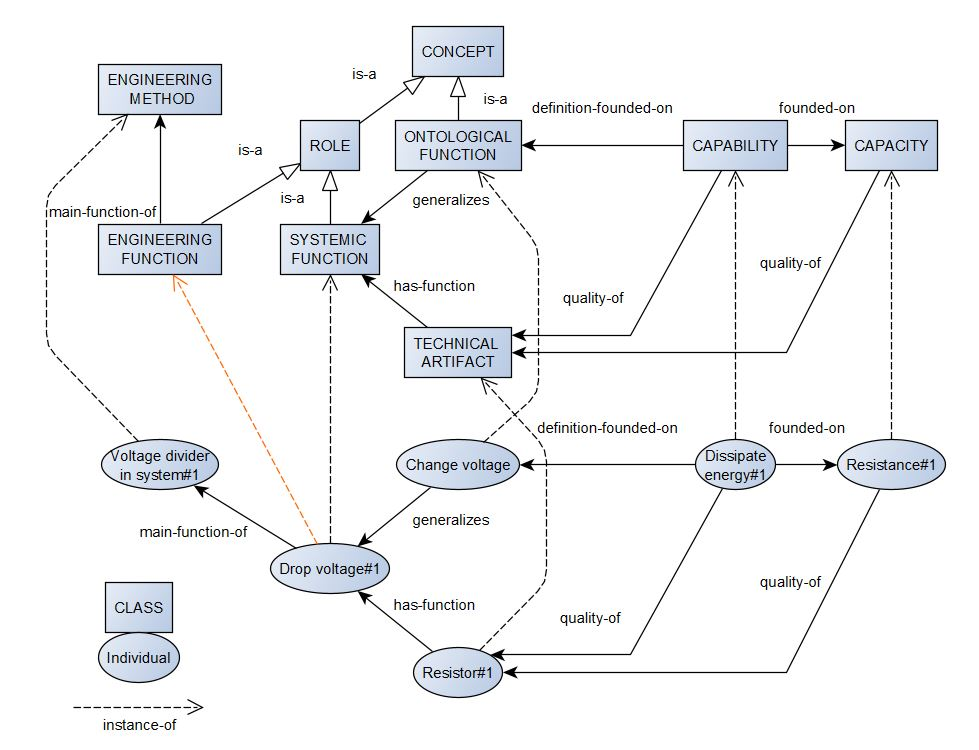
\includegraphics[width=0.95\textwidth]{schema-manuale.JPG}
    \caption{Main concepts and relations in the presented ontology. For simplicity and clarity, the picture refers to the OWL model and many relations and concepts have been suppressed. In addition, an instantiation of the schema for the case of a voltage divider is given. The red instance-of arrow is inferrable, since the related systemic function is main-function-of some engineering method (cfr. \refdf{def:engFunc}).}
    \label{fig:model}
\end{figure}

\medskip
We conclude this section with another example to show how the concepts we have introduced above concur to provide an integrated description of a functional scenario.\myComment{\footnote{Notice again the similarity with the work of Kitamura, Sasajima, Mizoguchi et al. \cite{kitamuraOntologybasedDescriptionFunctional2003}.}} Suppose that a company handling swimming pools must empty some of its pools for maintenance. This imposes a goal, say `the pools are empty', that must be carried out through some device able to realize a `to move' (ontological) function, specialized to a systemic function in the context of the swimming pool system.
Such a function can be realized by artifacts that have a corresponding capability. In this case, the function would probably be implemented through some fluid-emptying-method, that is, through the knowledge of the way that a recipient can be emptied, and its fluid content disposed of, by pressurizing the fluid and guiding it through a path.
%, and finally release it in a storage.
Now, the `pressurize' sub-function (which refers to the goal of `having a big enough pressure gradient') could be implemented through a pumping-method, that is, referring to engineering knowledge about pumps.
Then, a pump (more generally an artifact with pumping capability) could be selected for being the `doer' of the necessary `transform electrical energy into pressure' sub-sub-function.
In this context, we could say that the pump has been selected because of its pumping-capability and that the pumping-method describes, at least, a flow rate capacity, which founds the pumping-capability, and its interaction to the other properties and entities involved in the pumping process. 


%Chandrasakandar 2000 parla di behaviour come istanze (stati o cambiamento tra stati), eccetto che Beh-vi. The causal rules that describe the values of the variables under various conditions. che però non usa.

%%%%%

%not all expressible changings of state variables are possible: some could be logically inconsistent (e.g., the temperature is plus 20 and minus 2 degrees Celsius), some could be outside the realm of physics (e.g., a temperature in negative Kelvin degrees). The remaining are the possible changings of state variables. The remaining are 

%State variables are functions 
%Now, we assume that some state variables are intrinsic, for example the 

%A system has \firstTimeKeyWord{state variables}, that we take to be a primitive concept sumbsumed in qualities , that 
%We start from states,  

%, instead opting for representing behaviours as processes that require specific roles played by technical artifacts, such as the agent-like role that the pump plays in any pumping process.
%Additionally, we make use of the ontological category of DOLCE events, instead of processes, since we take behaviours to be occurred processes, and not 
%\bflist
%\item[\mydf{BehaviourConcrete}] $ \BehaviourConcrete{e} \myfi \DOLCEProcess{e} \land  \\ \exists y \participateAsDoer{y}{e}$ 
%\eflist

%%%%%% formalizzazione parte 3: funzioni

%Now we can finally talk about functions.
%We will mainly base our discussion on the work \cite{mizoguchiUnifyingDefinitionArtifact2016}, in that we will define functions in a way that intrinsically takes into account functional decomposition.

%We will make use, for our definition, of the concepts of behaviour, goal, context, and context...
%First we define a goal as a selected stative perdurant of a system  
%In the literature, the term \quotes{state} is commonly used, but we need to use \quotes{stative perdurant} instead. 
%his is because in \DOLCE the category of states is a strict subclass of stative perdurants, that, for example, excludes the buzzing action of a clapper, since the clapper, while buzzing, alternates between two different states.

%We say that the 

%We do not formally define the term \quotes{system}, since we assume, informally, that every technical artifact is the system of its own parts, and one can always see a technica


%%%%%%%%

%%%%%%%%

\section{Evaluation and possible applications}\label{sec:appendice}
%\TODOinline{[SB: assiomi e def in owl dovrebbero essere chiaramente distinti usando, e.g., \textbf{a14$_{owl}$}][FC:fatto]}
\subsection[meta]{Reduction to \OWL ontology}
To facilitate the deployment of our theory in applications, we present an \OWL version of the first-order logic formalization. 
This is standard practice, for at least the following reasons: first, \OWL is decidable, while first-order logic is not, so that reasoning tasks will terminate in finite time.\footnote{Though the complexity might be  exponential in general.\myComment{\TODO{citazione}}} Second, \OWL is a standard endorsed by the World Wide Web Consortium (W3C) and is part of the Semantic Web technology stack \cite{OWL2-QUICK-REFERENCE}, and is the language of choice for many ontologies in various domains \cite{OWL-ontology-repositories}.

Unfortunately, the computational properties of \OWL come with a tradeoff with respect to its expressibility, therefore, one has to simplify the first-order theory. 
The original theory remains essential as it constrains the intended meanings of the \OWL concepts and provides the `official reading' of the theory, it also helps to conceptually understand how the overall model is supposed to work. 

The first-order theory developed in the previous sections can be converted to \OWL language as is, except for the expressions where ternary relations are used, as well as those that necessarily need at least three arguments to be formulated. %as well as \refax{ax:capacPartialDef}, which necessarily needs at least three variables to be formulated.
For example, the definition of systemic-function-of \refdf{def:functionOf}%-\refdf{def:function}
\marginpar{\color{red}{ho tolto \refdf{def:function}}}, the instantiation-founding definition \refdf{def:founding}, and the engineering \methodsName{singular} schema \refdf{def:method} cannot be expressed in \OWL. 
In these cases we have to weaken the axioms. For instance, in \OWL we replace the definition of systemic functions with
\bflist
\item[\myax{functionOWL}$_{owl}$] 
\myalignspaceskip
\setlength{\jot}{0pt}% Inter-equation spacing
\begin{align*}
    \FunctionSysNullary\sqsubseteq &
    (\forall\mathtt{classifies}.\BehaviourConcreteNullary \sqcap \exists\causallyContrNullary.\GoalNullary) 
        \sqcap \\ & \exists\foundedNullary.\SystemNullary)
\end{align*}
\eflist
where $\mathtt{classifies}$ is the inverse relation of $\DOLCECLby{\cdot}{\cdot}{\cdot}$. In this way the fact that systemic functions are founded on systems is preserved. %and highlighted.

%classifies only 
%    (Behaviour
%     and (causally-contributes-to some Goal)
%     and (participated-by-doer some TechnicalArtifact))

Additionally, all the ternary temporalized relations used in the first-order version, such as $\DOLCECLby{\cdot}{\cdot}{\cdot}$ \myComment{, $\playAs{\cdot}{\cdot}{\cdot}$,} 
and $\hspace{0pt}\texttt{participateAsDoer}(\cdot,\cdot,\cdot)$, occur in the \OWL version with the temporal argument removed, i.e., as binary relations.
The link between the temporalized and non-temporalized relations can be interpreted in different ways \cite{TerkajOntologyIndustrialEngineering2022}. For example, one could state that the non-temporalized relation holds if and only if the temporalized relation holds whenever one of the relation arguments exists, what argument precisely depends on the relation. This is our choice for parthood \refdf{def:partConstant}, classification, temporal quale, and participation-like relations as shown by these \textit{meta-rules} aimed to show the intended interpretations: %\TODOinline{[SB: le f.le qui sotto dovrebbero avere la stessa numerazione delle iniziali ma restare chiaramente differenziate, ad es. usando  \textbf{d13$_{meta}$}][FC:fatto]}
\bflist
\item[\mydf{CLnontemp}$_{meta}$] $ \DOLCECLbyBinary{x}{y} \myiff ((\exists t \DOLCEPRE{x}{t}) \land \forall t (\DOLCEPRE{x}{t} \myfi  \DOLCECLby{x}{y}{t}))$ 
\item \mytext{$x$ is constantly classified by $y$ if and only if $x$ is classified by $y$ whenever $x$ exists}
\item[\mydf{Qualenontemp}$_{meta}$] $ \DOLCEQualeDirect{x}{y} \myiff ((\exists t \DOLCEPRE{x}{t}) \land \forall t (\DOLCEPRE{x}{t} \myfi  \DOLCEQualeTer{x}{y}{t}))$ 
\item \mytext{$y$ is a constant temporary quale of the quality $x$ if and only if $y$ is a temporary quale of $y$ whenever $x$ exists}
\item[\mydf{participationDoerNonTemp}$_{meta}$] $ \participateAsDoerBinary{x}{y} \myiff \exists t (\DOLCEPRE{y}{t}) \land \forall t (\DOLCEPRE{y}{t} \myfi \participateAsDoer{x}{y}{t})$
\item \mytext{$x$ constantly participates-as-doer to $y$ if and only if $x$ participates-as-doer to $y$ for the whole of $y$ duration}
\eflist
%and, thus, also for the play-as relation. 
One could also state that the non-temporalized relation holds if and only if the temporalized relation holds true at some time adopting the following \textit{meta-rule}:%. This is our choice for the participation relations, for example, for participation-as-doer: 
\bflist
\item[\myex{participationDoerNonTempBIS}$_{meta}$] $ \participateAsDoerBinary{x}{y} \myiff \exists t ~\participateAsDoer{x}{y}{t}$
\eflist
There are other possibilities. The choice of one over the others must be planned carefully depending on the application concerns, since this kind of changes affects the intended models of the \OWL ontology. For example, \refdf{def:participationDoerNonTemp} excludes participation-as-doer in, say, a chemical process only for its first part, while \refex{ex:participationDoerNonTempBIS} allows it, but in \OWL this difference is lost.
Additionally, the removal of the temporal argument reduces the flexibility of the ensuing ontology. For example, one cannot track (at least not directly) dynamic aspects of roles, e.g. a component that carries out a function at a time and then it changes its function. Nor one can express that, say, there is a chemical process which is driven by two different catalysts during its first and second parts.

Finally, as a further simplifying assumption, we define two binary relations that we will use as shortcuts to implement and simplify the definition schema  \refdf{def:method} and to redefine \refdf{def:engfunction}:
\bflist
  \item[\mydf{main-function-of}$_{meta}$] $ \mainFunction{\cst{f}}{\cst{m}} \myiff (\DOLCEConceptSubsum{\cst{f}}{\cst{main}^{\cst{m}}} \land \FunctionSys{\cst{f}}) $
  \item \mytext{$\cst{f}$ is main-function-of a \methodsName{singular} $\cst{m}$ if and only if it is a systemic function specializing the main-function role correspondig to $\cst{m}$} 
  \item[\mydf{sub-function-of}$_{meta}$] $ \subFunction{\cst{f}}{\cst{m}} \myiff (\DOLCEConceptSubsum{\cst{f}}{\cst{sub}^{\cst{m}}_i} \land \FunctionSys{\cst{f}}) $
  \item \mytext{$\cst{f}$ is main-function-of a \methodsName{singular} $\cst{m}$ if and only if it is a systemic function specializing any of the sub-function roles correspondig to $\cst{m}$} 
  \item[\mydf{engFunc}$_{owl}$] $ \FunctionEngNullary\equiv \exists\mainFunctionNullary.\MethodNullary$
  \item \mytext{Engineering functions are exactly the individuals that are main-function-of some engineering method}
\eflist

Note that in \refdf{def:engFunc} the individuals must necessarily be systemic functions due to \refdf{def:main-function-of}.

\begin{figure}[t]
  \centering
  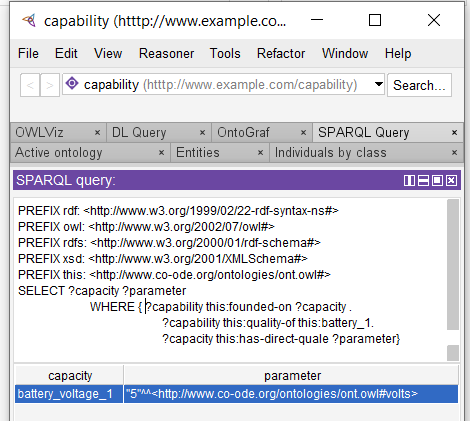
\includegraphics[width=0.7\textwidth]{query_screenshot.PNG}
  \caption{An implementation of \refCQ{CQ:capability-founded} in Protegé.\label{fig:screen_query}}
\end{figure}

\begin{figure}
  \centering
  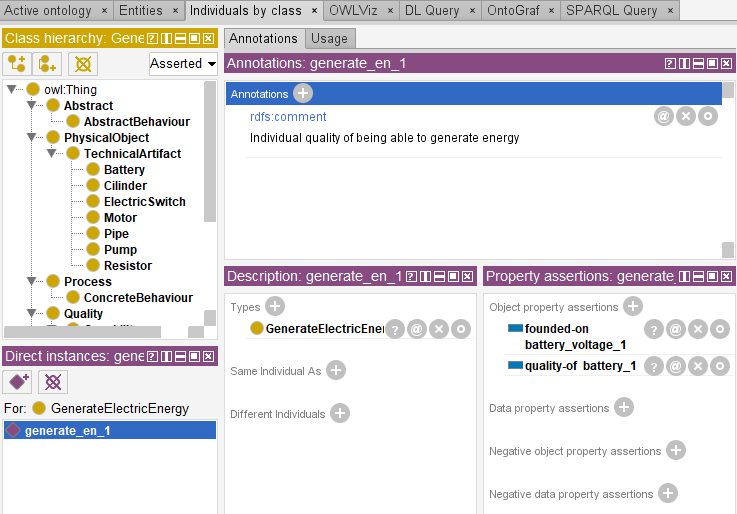
\includegraphics[width=0.8\textwidth]{entities_screenshot.PNG}
  \caption{A view of the ontology taxonomy in Protegé.\label{fig:screen_entities}}
\end{figure}\marginpar{\color{red}{IntQ e RelQ sono sottoclassi di PQ}}

Even though the \DOLCE ontology is primarily a first-order logic theory, \OWL versions exist as well, e.g. \DOLCE-lite and \DOLCE-Ultralite.\footnote{Available at \url{http://www.loa.istc.cnr.it/index.php/dolce/}.}
Any of these could be used to align the ontology developed in this paper with \DOLCE. In our case, we used the \OWL version of \DOLCE that has been recently submitted as part the ISO 21838 standard. %\footnote{\url{www.iso.org/standard/71954.html}.} 
The resulting ontology, which can be found on GitHub\footnote{\url{https://github.com/kataph/function-method-ontology.git}.}, was tested using the Hermit reasoner.
(For the sake of example, the ontology is populated with only a few individuals).


\subsection{Evaluation}
The ontology developed in this paper is a hand-crafted prototype that discusses middle and high-level concepts. 
Therefore, some common approaches to evaluation cannot be employed, as, for example, there is no \qquotes{gold standard} \cite{sfarGoldStandardBased2016}, or set of formal ontologies that one could use to compare common ontology metrics (such as those extracted by OntoMetrics\footnote{\url{https://ontometrics.informatik.uni-rostock.de/ontologymetrics/index.jsp}.}), nor there is a precise application against which to carry out the evaluation. 
Instead, we will evaluate our ontology using the OntoClean methodology  \cite{guarinoOverviewOntoClean2009} and the Ontology Pitfall Scanner \cite{poveda2014oops}. 
Moreover, we will discuss how our ontology answers the research questions \refRQ{RQ:RQ1}-\refRQ{RQ:RQ1.2}, as well as some competency questions that will serve to demonstrate the expressive potential of the ontology.
Finally, we will also discuss some possible application scenarios, though we highlight that the ontology main goals are the research questions \refRQ{RQ:RQ1}-\refRQ{RQ:RQ1.2}. The development of derived application-level ontologies is a goal for further work.

\paragraph{OntoClean.} OntoClean does not identify any issue in our taxonomy, that is, none of the meta-level rules that OntoClean methodology enforces are violated.
In fact, this is almost trivial to check: since we are extending \DOLCE categories, the only source of OntoClean violations would be an extension of role-concepts (that is, the set of all entities that, at a given time, are classified by the role-concept) which is not anti-rigid. 
This condition is not violated since (systemic) functions, as we define them, are contextual (e.g., a heat exchanger, with its behaviour, may be used either to heat a substance or to cool it, depending on the context). The other rules checked in the OntoClean methodology are trivially true. 
The correspondence with OntoClean principles is mainly due to the alignment of our theory with a well-established upper-level ontology. 

\paragraph{Ontology Pitfall Scanner} The \OWL ontology was evaluated with the Ontology Pitfall Scanner (OOPS!) \cite{poveda2014oops}, which searches for common design errors from a list of 41 items. Among the pitfalls not related to imported ontologies, the scanner found some minor stylistic issues\footnote{Some inverse object-properties are not declared explicitly, and the naming convention differs between object-properties and classes.} and warned about a few important pitfalls: P11 (\qquotes{Missing domain or range in properties}), P24 (\qquotes{Using recursive definitions}), and P30 (\qquotes{Equivalent classes not explicitly declared}). Of these three, P11 means that not every object property has domain and range axioms, but this is a conscious design choice to reduce the ontological commitment of the ontology. P24 occurs because OOPS! thinks that \refax{ax:functionAbstr} is a recursive definition (since the class of ontological functions appears both on the left and on the right of the material implication), but this is not the case. %\refax{ax:functionAbstr} is a normal axiom. 
Similarly, P30 occurs because OOPS! is, incorrectly, assuming that the class of resistors (capabilities) and the class of resistances (capacities) should be equivalent. %, perhaps based on the similarity in their names. 

% % The Ontology Pitfall scanner (OOPS!) evaluates an
% % ontology by searching for design pitfalls considered
% % from a catalogue of 41 common pitfalls in the ontology development process, classified in a three level
% % scale: critical, important and minor. Most of them (33
% % out of 41 pitfalls) can be identified semi-automatically
% % by OOPS!. The initial evaluation of ExtruOnt yielded
% % some flaws that were corrected, nonetheless, 2 minor
% % pitfalls remain due to external ontology imports. Table
% % 2 presents the evaluation summary made by OOPS!. --ExtruOnt

%12-Our ontology passed OntoClean and OOPS checks, but these were almost trivial due to the use of an upper ontology as reference, and to the small size of the ontology, respectively.
%Therefore, we turn to the competency questions methodology

% ("Can the authors identify any use cases, motivating scenarios, or competency questions that their ontology could address in real engineering design practices"):
\paragraph{Research questions and competency questions}
Our ontology answers the research questions listed in the introduction. 
In particular:
\begin{itemize}
  \item \textbf{Answer to \refRQ{RQ:RQ1}.} We modeled functions as \DOLCE-concepts that classify certain classes of perdurants. 
  This modelling choice explains how functions can exist even when they are not executed.
  Moreover, we separated functions into the distinct categories of engineering methods and (proper) functions, and, further, we separated functions into systemic or ontological depending on their abstraction level, thus explaining the ambiguity on the why-how or abstraction-implementation axes.
  \item \textbf{Answer to \refRQ{RQ:RQ1.1}.} Systemic functions can be decomposed as discussed in Subsection \ref{subsec:fun-dec}, where each decomposition is associated with an engineering \methodsName{singular}. %in such a way that an engineering method describes how a decomposition must happen. 
  \item \textbf{Answer to \refRQ{RQ:RQ1.2}.} We have characterized capabilities and capacities in Section \ref{sec:CapabilAndCapac}. In the first case we leveraged ontological functions, in the second case we suggested considering capacities as parameters of capabilities. Moreover, capabilities and capacities are clearly separated by the use of the founding relation: capabilities are founded on capacities, while the opposite does not hold.     
\end{itemize} 
Additionally, since the formal ontology answers these research questions, it is also able to answer related competency questions, which can be of interest in applications, such as the following:

\bflist
\item[\myCQ{first-function-capability}] Given an (ontological) function, which artifacts have the capability of satisfying it? %%IM
\item[\myCQ{function-implementation}] How can the given ontological function be implemented? %Given an (ontological or systemic) function, which methods can be employed to implement it? %%NIM
\item[\myCQ{capability-founded}] What are the capacities that a given capability is founded on?%Which parameters explain the performance of a capability or of a function? %%IMMAGINE
%\item[\myCQ{function-parameter}] Which characteristics of which components are involved in executing the \ontoFunc{fullPlural} present in a given system? %% RODONDANTE CON LA PROSSIMA
\item[\myCQ{function-parameter2}] Which parameters explain the performance of the \myComment{functions} some component in a given system? (If interpreted as \quotes{what are the capacities of the capabilities of the component that are relevant in executing its function?})\TODO{S: non sono sicuro di cosa intendi qui[FC:provato a chiarire]}
\item[\myCQ{function-decomposition}] Which is the functional decomposition of a given system? %%IM
%\item[\myCQ{function-implementation}] How can the given ontological function be implemented? RIDONDANTE
%\item[\myCQ{method-specialisation}] What does this engineering method need? RIMOSSA
\item[\myCQ{last-tag-function}] Which is the function of the given tag and what is its purpose?
\eflist

% 1 IM what components have a capability that corresponds to a given function:
% 2 what \methodsName{singular} could implement a given \ontoFunc{fullSingular}, 
% 3 what are the capacities that a given capability is founded on, 
% 3 IM in IMMAGINE what is their value for a given object (Figure \ref{fig:screen_query}). 
% 4 IM what capacities of what components are involved in executing the \ontoFunc{fullPlural} present in a given system:
% 5 IM For example, the following query takes a given system as inputs and returns all systemic functions involved in a \methodsName{singular}, with their role (main-function or sub-function) and underlying component:
% 6 Given some \ontoFunc{fullSingular}, one can set a query to return the list of \methodsName{plural}, present in the database, that can be implemented through systemic-function specialisation of the input \ontoFunc{fullSingular}; %% DUPLICATO
% 7 or explain what \methodsName{singular}-(sub)types specialize a given \methodsName{singular}, and what systemic-function-types are required by that \methodsName{singular}. RIMOSSO
% 8 Which is the function of this tag. 

%Of course, the RDF schema of our ontology supports many more competency questions, we chose some of the most interesting. 
%Additionally, many possible questions would not need our ontological analysis of functions and related concepts at all to be formulated (e.g., \qquotes{what is the value of a certain property of the given component}).
% \bflist
% \item[\myCQ{cq1}] What is the function of a given component?
% \item[\myCQ{cq1bis}] What is the value of a given property of a given component?
% \item[\myCQ{cq1tris}] What is the value of a given property of a given component?
% \eflist

The \OWL ontology, after being populated, can be used to answer the competency questions \refCQ{CQ:first-function-capability}-\refCQ{CQ:last-tag-function} by means of SPARQL queries. 
For example, these are implementations of \refCQ{CQ:first-function-capability}:
\begin{verbatim}
  PREFIX : <https://github.com/kataph/function-method-ontology#>
  SELECT  ?component
  WHERE { 
    ?capability :definition-founded-on :<the given function> .
    ?capability :quality-of ?component}
\end{verbatim}
of \refCQ{CQ:function-parameter2}:
\begin{verbatim}
  PREFIX : <https://github.com/kataph/function-method-ontology#>
  SELECT  ?component ?functionOntological ?capacity
  WHERE { 
          ?functionSystemic :function-of ?component .
          ?functionSystemic :founded-on :<the given system> .
          ?functionSystemic :specializes ?functionOntological .
          ?capability :definition-founded-on ?functionOntological .
          ?capability :quality-of ?component .
          ?capability :founded-on ?capacity .
          ?capacity :quality-of ?component}
\end{verbatim}
and of \refCQ{CQ:function-decomposition}, provided that the functional decomposition of a system is interpreted as the list of all systemic functions of the given system involved in a \methodsName{singular}, with their role (main-function or sub-function) and underlying component:
\begin{verbatim}
  PREFIX rdf: <http://www.w3.org/1999/02/22-rdf-syntax-ns#>
  PREFIX rdfs: <http://www.w3.org/2000/01/rdf-schema#>
  PREFIX : <https://github.com/kataph/function-method-ontology#>
  SELECT  ?component ?functionSystemic ?role ?method 
  WHERE { 
      ?functionSystemic ?role ?method .
      ?method rdf:type/rdfs:subClassOf* :EngineeringMethod .
      ?functionSystemic :function-of ?component  .
      ?component :constant-part-of :<the given system>}
\end{verbatim}
The remaining competency questions can be implemented in a similar way (see also Fig.\ref{fig:screen_query} for \refCQ{CQ:capability-founded}).\TODO{S: check [FC: I thick I checked]}

\medskip
The fact that our ontology can answer all these questions shows its expressivity and coverage.
In the following paragraphs we explain how these characteristics could be used in application scenarios.

% Motivating scenarios:

\subsection{Motivating scenarios}
%The previous [1-2] queries showcase the possibility of linking capabilities to functions. This is important for one could develop, based on this link, an application allowing engineers to find whether they already have available components that can satisfy a given functional requirement, e.g. in early system design.
\paragraph{Innovative Design (and other things).}
A good portion of the literature on functional modelling argues that functional modelling can be used to improve engineering design.
For instance, the basic argument of the approach of Pahl and \cite{pahl_engineering_2007} is as follows: designers should start from the customer's requirements, translate them into high-level functions, then decompose those functions into less abstract ones, until arriving at a point where finding a solution that realizes the functions is easy.
This methodology, is argued, facilitates engineers to quickly develop high-quality designs and enhances their creativity by decoupling the goals of the design from the ways they are achieved.

This argument is not wrong, but, in actual practice, one rarely starts from a blank slate. 
Designers are typically constrained by the need to reuse pre-existing solutions, for a company may have developed a legacy that is difficult to depart from, possibly because the company would not be able to (profitably) reroute its know-how and resources towards innovative lines of products, or other reasons.
Therefore, designers usually have to devise marginal improvements or corrections in pre-existing solutions, and these activities seem at odds with the aforementioned methodology. % or ways to readapt them for marginally more general situations. 
Additionally, the described methodology is design-oriented and does not seem relevant to other activities, such as troubleshooting or reverse engineering, despite functional reasoning being clearly relevant in all of them.

One important reason for carrying out ontological analysis is to bridge all such activities and cases, by producing an explicit representation (the ontology) of the shared conceptualisation of the relevant stakeholders, which can be used by all of them.
We argue that our ontology is useful for the blank-slate innovation scenario (for, e.g., competency questions \refCQ{CQ:first-function-capability} and \refCQ{CQ:capability-founded} showcase the possibility of linking capabilities to functions, which is important since it allows engineers to find whether they already have available components that can satisfy a given functional requirement), as well as many other scenarios, some of which we describe briefly in the following. 

\paragraph{Incremental innovation} In a company, innovation may happen mainly through incremental changes in pre-existing products. 
Therefore, product types will have a version history. %, in which each new version improves on the former. 
Using our ontology, one could describe %some
%\footnote{For example, our ontology by itself is not able to express the case, which is typical, that a new version of a product has been released to repair a known widespread issue.} \TODO{S: non ho capito, meglio togliere}
the relevant improvements, allowing their digitalisation in a semantically meaningful way. 
For instance, a new version may introduce new capabilities, or it may have the same capabilities as the former version, but it could realize them better due to different capacities. 
Storing such information could be more helpful to engineers than just storing structural information (like the bill of material) of the different versions in the enterprise management system.

\paragraph{Knowledge transfer} An engineer or technician could have recently been employed by a manufacturing company. 
In that case, he or she is (hopefully) trained to learn about the company's products and their functioning. 
Still, a good part of the knowledge the company possesses, especially functional knowledge, is implicit. 
Therefore, the trainee will learn about it only through experience or through his/her background knowledge of the domain. 
This may be a slow process, and some knowledge could be lost. 
Building a knowledge base modelling functional knowledge (necessarily together with other types of information, e.g. geometrical from CAD models, etc.) could facilitate training since it would relieve the trainee from having to infer the functionality of components from their structure, as well as the (functional) role of components within their systems. 
%Additionally, maintaining a knowledge base of engineering methods could be an effective way to record the company's know-how, which may very well be unique to that company, and, therefore,  

\paragraph{Troubleshooting} When a technician troubleshoots a product he often makes use of functional reasoning (e.g., \qquotes{the volume of the speakers is constantly louder than it should be. It may be that there is something wrong with the amplifier circuit, since it is that component that has the function of controlling the volume}). 
Sometimes, a technician may lack sufficient knowledge about the functional structure of a product to carry out such reasoning fruitfully (say, it is an external contractor with limited knowledge of the company which manufactures the product). 
In those cases, a clear rapresentation of the product functional structure, if accessible to the technician, may solve the issue.
For example, a query answering \refCQ{CQ:function-parameter2} may be useful in this  case.

\paragraph{Formal Requirements.}
Requirements are an essential part of engineering design, which engineers have to write, share, maintain, and implement. 
The ensuing work and documentation can be daunting, especially in large progects. Therefore, attempts have been made to standardize \cite{alrumaihDomainOntologyRequirements2020}, trace \cite{murtazinaOntologybasedApproachSupport2019}, and automatize \cite{holterScopeDetectionTextual2021} requirement pipelines using ontologies. 
%Some of these approaches discuss properties of requirements themselves, for example, they build a taxonomy of requirement types %\TODO{[cit]} or they develop vocabularies for the activities carried out during requirement managememnt %\TODO{[cit]}. 
Some approaches discuss how requirements should be written, so that their quality, shareability, and even automatic verification against a design model can be assured (e.g., \cite{jinxinlinRequirementOntologyEngineering1996, chenOntologybasedRequirementVerification2020}).
In the latter case, requirements are usually interpreted as assertions (constraints) about an engineering artifact that can be expressed (at least some of them can) in a formal language. 
The fact that the requirement refers to something that \textit{should be}, and not to something that \textit{is}, means that requirements are modal concepts, though this can be left implicit in formal representations.  
For example, a requirement translated directly from a client's request, could be that the product, say a table, \qquotes{must weight as little as possible}, then engineers could precise this in different ways, e.g., by stating 
\bflist
  \item[\myex{req1}] $ weight(table\_top) \leq 5kg \land weight(i_{th}\_table\_leg) \leq 2kg$, for $i = 1,2,3,4$. 
\eflist
Therefore, if one also designs products using the same formal language, the products can be checked against the set of constraints, to verify that those are satisfied by the products.

One difficulty of this approach is that some requirements are more difficult to express than others.
Requirements such as \refex{ex:req1} are easy to express, as they refer to physical properties of the products (they are sometimes called \qquotes{physical requirements} \cite{jinxinlinRequirementOntologyEngineering1996}).
On the other hand, requirements linked to product performance or functions are more difficult to express.
For example, in \cite{jinxinlinRequirementOntologyEngineering1996}, the requirements \qquotes{The artifact [desk spot lamp] should be able to illuminate more than half a square meter of room}, \qquotes{The base [of the desk spot lamp] should provide support to the artifact}, and \qquotes{the short arm must have a hole [\dots]} are formalized as follows: 
\bflist
  \item[\myex{req2}] $ arm(p) \myfi \exists f(hole\_feature(f) \land
 feature\_of(f, p) \land
  $ [\dots]. 
  \item[\myex{req3}] $ desk\_spot\_lamp(p) \myfi \exists f( illuminating\_feature(f) \land feature\_of(f, p) \land illumination\_area(f) \geq 0.5 $
  \item[\myex{req4}] $ base(p) \myfi \exists f (provide\_support\_feature(f) \land feature\_of(f, p) $ 
\eflist
Therefore, predicates \qquotes{$illuminating\_feature$}, \qquotes{$provide\_support\_feature$}, and \qquotes{$hole\_feature$} are introduced to classify the capability to illuminate, the function to support, and the hole of the short arm as \qquotes{$feature\_of$} the corresponding artefacts. 
So that capabilities and functions are features in the same sense that a hole is, and we consider this an ontological error\footnote{For example, in \DOLCE features form a category of endurants that are (generically constantly) dependent on physical objects that cannot be detached from their corresponding physical object without losing their identities. In this sense, a hole is a feature, while the wheel of a car is not. The fact that, in our approach, features are not capabilities or functions, entailed by our categorisation of those as qualities and non-physical endurants, respectively.}.

The point is that being able to express requirements that mention capabilities or functions is difficult, and an ontology describing such concepts would make things easier.
For example, using our theory we would write requirements \refex{ex:req3} and \refex{ex:req4} as, respectively (in the following we have introduced a subclass of capabilities, $illuminating\_capability$, a subclass of capacities $illumination\_area$, and a subclass of (ontological) functions, $provide\_support$):
\bflist
  \item[\myex{req5}] $ desk\_spot\_lamp(p) \myfi \exists f,c,v( illuminating\_capability(f) \land \DOLCEQualityDirect{f}{p} \land illumination\_area(c) \land \\ \founded{f}{c} \land \DOLCEQualeDirect{c}{v} \land \DOLCEPartBin{v}{[0.5, \infty)}$
  \item[] \mytext{Every desk spot lamp has a capability to illuminate, founded on an illumination-area-capacity greater than 0.5} 
  \item[\myex{req6}] $ base(p) \myfi \exists f_o,f_s (provide\_support(f_o) \land \DOLCECLbyBinary{f_s}{f_o} \land \FunctionSysOf{f_s}{p})$
  \item[] \mytext{Every lamp base has a (systemic) function of (ontological-function-)type provide support} 
\eflist
Notice that \refex{ex:req5} and \refex{ex:req6} can be readily rewritten in \OWL, so that they can be part of an \OWL knowledge base containing all the requirements that can be expressed in a similar way. 
Then, if engineers build during design a model of the product, using the same language, they just need to import the model into the knowledge base with the requirements: the product model satisfies the requirements if and only if the ensuing ontology is consistent (similarly one can find if the requirements are inconsistent or if there are duplicates).  
In an actual application the user may never write complex formulas such as \refex{ex:req5} and \refex{ex:req6}, unless user-friendly templates are made available as done in \cite{chenOntologybasedRequirementVerification2020}.  

An analogous procedure is the one that the READI project \cite{overliAssetInformationModelling2021,kluwerOntologybasedRequirementsManagement2018} aims to implement. 
In their case, the requirement are expressed in SCD (Scope Condition Demand) form.
This means that they are assertions of the form
\bflist
  \item[\myex{SCD}] $ \text{S} \sqcap \text{C} \sqsubseteq \text{D}  $
\eflist
where S, C, and D are \OWL classes, for example (the example is taken from \cite{overliAssetInformationModelling2021}), \qquotes{Equipment with a transport dry weight above 1000 kg shall be weighed by the manufacturer and a weight certificate shall be issued} is written in such a form, if S, C, and D are interpreted as the classes \quotes{Equipment}, \quotes{things with transport dry weight above 1000 kg}, \quotes{things that have a weight certificate}, respectively.   
Again, it is difficult to express functions- and performance-related requirements in the format of \refex{ex:SCD} if one lacks an appropriate reference ontology. 

%To summarize, using our ontology, one could enhance current work aimed at the digitalisation of written requirements, by facilitating the assertion of requirements related to product performance and functions.


%%%%%%%%%%%%%%%%%%%%%%%%%%%
%%%%%%%%%%%%%%%%%%%%%%%%%%%
%%%%%%%%%%%%%%%%%%%%%%%%%%%
\myComment{
The \OWL ontology, after being populated, can be used to query information about the functionality of objects. For example, one could query what \methodsName{singular} could implement a given \ontoFunc{fullSingular}, or what are the capacities that a given capability is founded on, and what is their value for a given object (Figure \ref{fig:screen_query}). Moreover, one could query  
what components have a capability that corresponds to a given function:
\begin{verbatim}
  PREFIX : <https://github.com/kataph/function-method-ontology#>
  SELECT  ?component
	WHERE { 
    ?capability :definition-founded-on :<the given function> .
    ?capability :quality-of ?component}
  \end{verbatim}
\begin{comment}PREFIX rdf: <http://www.w3.org/1999/02/22-rdf-syntax-ns#>
PREFIX owl: <http://www.w3.org/2002/07/owl#>
PREFIX rdfs: <http://www.w3.org/2000/01/rdf-schema#>
PREFIX xsd: <http://www.w3.org/2001/XMLSchema#>
PREFIX this: <https://github.com/kataph/function-method-ontology#>
SELECT  ?component
	WHERE { ?capability this:definition-founded-on this:convert_chemical_energy_into_electricity_1 .
		?capability this:quality-of ?component}
\end{comment}
or what capacities of what components are involved in executing the \ontoFunc{fullPlural} present in a given system:
\begin{verbatim}
PREFIX : <https://github.com/kataph/function-method-ontology#>
SELECT  ?component ?functionOntological ?capacity
WHERE { 
		    ?functionSystemic :function-of ?component .
		    ?functionSystemic :founded-on :<the given system> .
		    ?functionSystemic :specializes ?functionOntological .
		    ?capability :definition-founded-on ?functionOntological .
		    ?capability :quality-of ?component .
		    ?capability :founded-on ?capacity .
		    ?capacity :quality-of ?component}
\end{verbatim}
\begin{comment}
PREFIX rdf: <http://www.w3.org/1999/02/22-rdf-syntax-ns#>
PREFIX owl: <http://www.w3.org/2002/07/owl#>
PREFIX rdfs: <http://www.w3.org/2000/01/rdf-schema#>
PREFIX xsd: <http://www.w3.org/2001/XMLSchema#>
PREFIX this: <https://github.com/kataph/function-method-ontology#>
SELECT  ?component ?capacity
	WHERE { 
		?component this:part-of this:electrical_circuit_1 .
		?functionSystemic this:founded-on this:electrical_circuit_1 .
		?functionSystemic this:specializes ?functionOntological .
		?capability this:definition-founded-on ?functionOntological .
		?capability this:quality-of ?component .
		?capability this:founded-on ?capacity .
		?capacity this:quality-of ?component}
  \end{comment}
The previous queries showcase the possibility of linking capabilities to functions. This is important for one could develop, based on this link, an application allowing engineers to find whether they already have available components that can satisfy a given functional requirement, e.g. in early system design.

The ontology also supports queries related to engineering \methodsName{plural} and their relation with functions.
For example, the following query takes a given system as inputs and returns all systemic functions involved in a \methodsName{singular}, with their role (main-function or sub-function) and underlying component:
\begin{verbatim}
PREFIX rdf: <http://www.w3.org/1999/02/22-rdf-syntax-ns#>
PREFIX rdfs: <http://www.w3.org/2000/01/rdf-schema#>
PREFIX : <https://github.com/kataph/function-method-ontology#>
SELECT  ?component ?functionSystemic ?role ?method 
WHERE { 
    ?functionSystemic ?role ?method .
    ?method rdf:type/rdfs:subClassOf* :EngineeringMethod .
    ?functionSystemic :function-of ?component  .
    ?component :constant-part-of :<the given system>}
\end{verbatim}
\begin{comment}
PREFIX rdf: <http://www.w3.org/1999/02/22-rdf-syntax-ns#>
PREFIX rdfs: <http://www.w3.org/2000/01/rdf-schema#>
PREFIX : <https://github.com/kataph/function-method-ontology#>
SELECT  ?component ?functionSystemic ?verb ?method
	WHERE { ?functionSystemic ?verb ?method .
		?method rdf:type/rdfs:subClassOf* :EngineeringMethod .
		?functionSystemic :function-of ?component }
\end{comment}
Given some \ontoFunc{fullSingular}, one can set a query to return the list of \methodsName{plural}, present in the database, that can be implemented through systemic-function specialisation of the input \ontoFunc{fullSingular}; or explain what \methodsName{singular}-(sub)types specialize a given \methodsName{singular}, and what systemic-function-types are required by that \methodsName{singular}. 
This is useful, both during design, since it gives information about how to implement a given function, and during reverse engineering since it explains how the parts of a system cooperate to carry out a function of coarse granularity. 

Even though the \DOLCE ontology is primarily a first-order logic theory, \OWL-adapted versions exist, such as \DOLCE-lite or \DOLCE-Ultralite\footnote{Both openly available, e.g., at \url{http://www.loa.istc.cnr.it/dolce/overview.html}.}. 
Any of these could be used to align the ontology developed in this paper with \DOLCE. In our case, we used the \OWL version of \DOLCE submitted as part of the ISO 21838 standard.%\footnote{\url{https://www.iso.org/standard/71954.html}.} 
The resulting ontology, which can be found on GitHub\footnote{\url{https://github.com/kataph/function-method-ontology.git}.}, was tested using the Hermit reasoner.
(For the sake of example, the ontology is populated with a few individuals).}
%%%%%%%%%%%%%%%%%%%%%%%%%%%
%%%%%%%%%%%%%%%%%%%%%%%%%%%
%%%%%%%%%%%%%%%%%%%%%%%%%%%


\section{Conclusion}\label{sec:conc}
%%non riassuntive, bensi' esplicative
%% abbiamo fatto X, nel farlo abbiamo usato approcci (riichiro, ecc., quelli che abbiamo usato, emilio, qualche standard, - ci siamo appoggiati su questa roba- dolce incluso, e cosa è novelty? E' validazione ontologica, aver chiarito come concetualizzare queste funzioni in modo sistematico in framework ontologico unico. Essere onesti nel dire che la roba nuova che vi formiamo è stata questa qua e basata su quella la.)
The work presented in this paper contributes to the ontological understanding and modeling of fundamental concepts used in engineering, especially functionality.
In particular, we have shown how one can give ontologically-grounded definitions of capability, capacity, behaviour, and function using first-order logic.
Moreover, we have shown how one can use an ontology and the notion of functional decomposition to distinguish between ontological, systemic, and engineering functions, and how \ontoFunc{fullPlural} can be used to explain the difference between capabilities and capacities.
Finally, we partially translated our first-order theory in \OWL, showcasing a preliminary serialisation of our theory in a computer-friendly formal language.

Our approach builds on a series of previous works, especially on the study of functionality carried out by engineers and researchers, in particular \cite{pahl_engineering_2007, sasajimaFBRLFunctionBehavior1995,mizoguchiUnifyingDefinitionArtifact2016}; the study of resources in manufacturing, in the applied ontology literature as well as some standards  \cite{sanfilippoResourcesManufacturing2015, borgoCapabilitiesCapacitiesFunctionalities2021, jochemISOISO15531312004}; and the top-level ontology \DOLCE and its developments \cite{masoloSocialRolesTheir2004, masoloWonderWebDeliverableD182003,borgoDOLCEDescriptiveOntology2022}.
This work relies on an in-depth ontological analysis of the domain, which,  exploiting the characteristics of the \DOLCE ontology, clarifies the conceptualisation of functions and related concepts in a systematic way.

We evaluated the quality of our implementation by assessing the clarity, expressive capability, and flexibility of our ontology with respect to some research questions, some competency questions, and some application scenarios. 
The relevance of our work is highlighted by the ability to answer a series of questions, from \refRQ{RQ:RQ1}-\refRQ{RQ:RQ1.2} to \refCQ{CQ:first-function-capability}-\refCQ{CQ:last-tag-function}, showing that the ontology could be able to support applications in most engineering scenarios where functional reasoning is required. 

This paper has set the vision and the core elements of our theory, yet many things require further work and testing to achieve a  level of detail and coverage suitable for real applications.
For example, linking the notions of behaviour to the modelling equations that engineers use to simulate a system is a topic that has not been addressed and requires additional research. Similarly, we need to analyze more in-depth how an ontological approach based on our theory can help to make uniform the description of application scenarios, starting from those touched upon in the paper.


%%They then use these equations to analyze or predict how well the artifact would realize its functional requirements. I think if the authors could bridge these notions (behaviors, states, and modelling equations), it could be another important contribution of the paper. - cit. revisore 3

%\TODO{<--FC:check if ok.}
%\begin{figure}[t]
%\includegraphics{}
%\caption{Figure caption.}\label{f1}
%\end{figure}

%\begin{table*}
%\caption{} \label{t1}
%\begin{tabular}{lll}
%\hline
%&&\\
%&&\\
%\hline
%\end{tabular}
%\end{table*}

\section*{Acknowledgments}

%%%% NOTA:
%Tutte le pubblicazioni scientifiche eventualmente prodotte dal/dalla 
%dottorando/a che usufruisce della borsa finanziata dalla presente 
%Convenzione e derivate dall'attività svolta nell'ambito del ciclo 
%di dottorato, oltre a indicare l'afferenza al Dottorato dell'Università,
%dovrà citare il sostegno all'attività di ricerca da parte del Finanziatore.

The authors acknowledge support by the European project OntoCommons (GA 958371, \url{www.ontocommons.eu}). Francesco Compagno is funded by the company Adige Spa. 
The authors wish to thank Riichiro Mizoguchi for the precious time spent discussing his work as well as the topics of function definition and engineering function modelling.


%%%%%%%%%%% The bibliography starts:

%%%%%%%%%%%%%%%%%%%%%%%%%%%%%%%%%%%%%%%%%%%%%%%%%%%%%%%%%%%%%
%%                  The Bibliography                       %%
%%                                                         %%
%%  ios1.bst will be used to                               %%
%%  create a .BBL file for submission.                     %%
%%                                                         %%
%%                                                         %%
%%  Note that the displayed Bibliography will not          %%
%%  necessarily be rendered by Latex exactly as specified  %%
%%  in the online Instructions for Authors.                %%
%%                                                         %%
%%%%%%%%%%%%%%%%%%%%%%%%%%%%%%%%%%%%%%%%%%%%%%%%%%%%%%%%%%%%%


%\nocite{*}
% if your bibliography is in bibtex format, use those commands:
\bibliographystyle{ios1}           % Style BST file.
\bibliography{bibliography}        % Bibliography file (usually '*.bib')

% or include bibliography directly:
%\begin{thebibliography}{0}
%\bibitem{r1} F. Author, Information about cited object.
%
%\bibitem{r2} S. Author and T. Author, Information about cited object.
%\end{thebibliography}

\end{document}
